\addtocontents{toc}{\protect\setcounter{tocdepth}{1}}
\hypersetup{bookmarksdepth=2}
\chapter{BASIC 65 Command Reference}

\section{Commands, Functions and Operators}

This appendix describes each of the commands, functions and other
callable elements of BASIC 65, which is an enhanced version of BASIC 10.
Some of these can take one or more arguments, which are pieces of input
that you provide as part of the command or function call.
Some also require that you use special keywords.
Here is an example of how commands, functions and operators will be
described in this appendix:

{\bf KEY <numeric expression>,<string expression> }

In this case, KEY is what we call a \textbf{keyword}. That just means
a special word that BASIC understands.
Keywords are always written in CAPITALS, so that you can easily
recognise them.

The {\bf <} and {\bf >} signs mean that whatever is between them must
be there for the command, function or operator to work.
In this case, it tells us that we need to have a
{\bf numeric expression} in one place, and a {\bf string expression}
in another place.
We'll explain what they are a bit more in a few moments.

You might also see square brackets around something. For example,
{\bf [,numeric expression]}.
This means that whatever appears between the square brackets is
optional, that is, you can include it if you need to, but
that the command, function or operator will work just fine without it.
For example, the {\bf CIRCLE} command has
an optional numeric argument to indicate if the circle should be filled
when being drawn.

The comma, and some other symbols and punctuation marks just represent themselves.
In this case, it means that there must be a comma between the
{\bf numeric expression} and the {\bf string expression}.
This is what we call syntax: If you miss something out, or put the
wrong thing in the wrong place, it is called a
syntax error, and the computer will tell you if you have a syntax error
by giving a \screentext{?SYNTAX ERROR} message.

There is nothing to worry about if you get an error from the computer.
Instead, it is just the computer's way of telling you that something
isn't quite right, so that you can more easily
find and fix the problem.
Error messages such as this won't hurt the computer or cause any damage to your program,
so there is nothing to worry about.
For example, if we accidentally left the comma out, or replaced it with
a full stop, the computer will respond with
a SYNTAX ERROR, similar to what's shown below:

\newpage
\begin{tcolorbox}[colback=black,coltext=white]
\verbatimfont{\codefont}
\begin{verbatim}
KEY 8"FISH"

?SYNTAX ERROR

KEY 8."FISH"

?SYNTAX ERROR
\end{verbatim}
\end{tcolorbox}


It is very common for commands, functions and operators to use one or
more {\bf``expressions''}.
An expression is just a fancy name for something that has a value.
This could be a string (\screentext{"HELLO"}), a number
(\screentext{23.7}), or a calculation that might include
one or more functions or operators (\screentext{LEN("HELLO") * (3 XOR 7)}).
Generally speaking, expressions can result in either a string or a numeric result.
In this case we call the expressions either string expressions or numeric expressions.
For example, \screentext{"HELLO"} is a {\bf string expression}, while
\screentext{23.7} is a {\bf numeric expression}.

It is important to use the correct type of expression when writing your programs.
If you accidentally use the wrong type, the computer will give you a
\screentext{?TYPE MISMATCH ERROR}, to say that the type
of expression you gave doesn't match what it expected. For example, we will get a
\screentext{?TYPE MISMATCH ERROR} if we type the following command,
because \screentext{"POTATO"} is a string expression instead of a numeric expression:

\begin{tcolorbox}[colback=black,coltext=white]
\verbatimfont{\codefont}
\begin{verbatim}
  KEY "POTATO","SOUP"
\end{verbatim}
\end{tcolorbox}

If you wish, you can try typing this in yourself.

Commands are statements that you can use directly from the {\bf READY.}
prompt, or from within a program, for example:

\begin{tcolorbox}[colback=black,coltext=white]
\verbatimfont{\codefont}
\begin{verbatim}
  PRINT "HELLO"
  HELLO

  10 PRINT "HELLO"
  RUN
  HELLO
\end{verbatim}
\end{tcolorbox}

\newpage
\section{BASIC 65 constants}

{\ttfamily
\setlength{\tabcolsep}{1mm}
\begin{center}
\begin{tabular}{|l|l|l|}
\hline
 type                   & example & example \\
\hline
decimal integer         &  32000  & -55       \\
decimal fixed point     &  3.14   & -7654.321 \\
decimal floating point  &  1.5E03 & 7.7E-02   \\
hex                     &  \$D020 & \$FF      \\
string                  & "X"     & "TEXT"    \\
\hline
\end{tabular}
\end{center}
}

\section{BASIC 65 variables}

Each scalar variable consumes 8 bytes of storage in memory.
The reserved area in bank 0 from \$F700-\$FEFF can store 256 variables.
Variables don't need to be declared, the type is determined by an appended
character. All variables without an appended character are regarded as REAL by default.
The storage is claimed at their first usage and they are initialised to zero,
string variables are initialised as an empty string "".

{\ttfamily
\setlength{\tabcolsep}{1mm}
\begin{center}
\begin{tabular}{|l|l|l|l|}
\hline
 type                   & appended character & range    & example  \\
\hline
byte                    &    \&    & 0 .. 255        & BY\& = 23 \\
integer                 &    \%    & -32768 .. 32767 & I\% = 5    \\
real                    &   none   & -1E37 .. 1E37   & XY = 1/3   \\
string                  &    \$    & length = 0 .. 255 & AB\$ = "TEXT" \\
\hline
\end{tabular}
\end{center}
}

\section{BASIC 65 arrays}

Each array consumes the number of elements multiplied by the item size
plus the size of the header (6 + 2 * dimensions) in memory.
For example the array
\begin{tcolorbox}[colback=black,coltext=white]
\verbatimfont{\codefont}
\begin{verbatim}
100 DIM X(8,2,3) :REM (0..8, 0..2, 0..3)
\end{verbatim}
\end{tcolorbox}
has 3 dimensions and 9 x 3 x 4 = 108 items.
The size for real items is 5, so the data of that array occupies 540 bytes.
The header size is 6 + 2 * 3 = 12 bytes.
So the total length in memory is 552 bytes.

Arrays are stored in bank 1 starting at address \$2000 and expand upwards.
They share the available memory (\$2000 .. \$F6FF) with the string area,
which starts in bank 1 at address \$F6FF and expand downwards.
Each of the above scalar variable types can be used as an array by declaring
them with a DIM statement. The arrays are initialised to zero for all
elements on declaration. If an undeclared array element is used,
an automatic implicit declaration is done, which sets the upper  boundary
for each dimension to 10. For example, the usage of an undeclared element
AB(3,5) would automatically perform a "DIM AB(10,10)".
The lower boundary for each dimension is always 0 (zero),
so an array initialised with DIM AB(10) consists of 11 elements and accepts indexes from
0 to 10.

String arrays are, more precisely expressed, arrays of string
descriptors. Each item consists of three bytes, which hold
the values: length of the string and the address (low/high byte)
of the assigned string in string memory.
The usage of the BASIC function POINTER with a string or
string array element as the argument, returns the address of the descriptor, not the string itself.

{\ttfamily
\setlength{\tabcolsep}{1mm}
\begin{center}
\begin{tabular}{|l|l|l|l|l|}
\hline
\multicolumn{2}{|c|}{type \& item size} & appended  & range    & example  \\
\multicolumn{2}{|c|}{}                  & character &          &          \\
\hline
byte     array &  1     &    \&    & 0 .. 255        & BY\&(5,6) = 23 \\
integer  array &  2     &    \%    & -32768 .. 32767 & I\%(0,10) = 5    \\
real     array &  5     &   none   & -1E37 .. 1E37   & XY(I\%) = 1/3   \\
string   array &  3     &    \$    & length = 0 .. 255 & AB\$(X) = "TEXT" \\
\hline
\end{tabular}
\end{center}
}

\section{BASIC 65 operators}

\subsection{unary numeric operators}

{\ttfamily
\setlength{\tabcolsep}{1mm}
\begin{center}
\begin{tabular}{|l|l|l|l|l|}
\hline
name & symbol & description & operand type & example \\
\hline
plus  & +   & positive sign & numeric & A = +42 \\
minus & -   & negative sign & numeric & B = -42 \\
\hline
\end{tabular}
\end{center}
}

\subsection{binary numeric operators}

{\ttfamily
\setlength{\tabcolsep}{1mm}
\begin{center}
\begin{tabular}{|l|l|l|l|l|}
\hline
name & symbol & description & operand type & example \\
\hline
plus           & +   & addition       & numeric & A = B + 42\\
minus          & -   & subtraction    & numeric & B = A - 42\\
asterisk       & *   & multiplication & numeric & C = A * B\\
slash          & /   & division       & numeric & D = B / 13\\
uparrow & $\uparrow$   & exponentiation & numeric & E = 2 $\uparrow$ 10\\
\hline
\end{tabular}
\end{center}
}

\subsection{relational operators}

{\ttfamily
\setlength{\tabcolsep}{1mm}
\begin{center}
\begin{tabular}{|l|l|l|l|}
\hline
symbol & description & operand type & example \\
\hline
 >   & greater          & numeric & A > 42  \\
 >=  & greater or equal & numeric & B >= 42 \\
 <   & less             & numeric & A < 42  \\
 <=  & less    or equal & numeric & B <= 42 \\
 =   & equal            & numeric & A = 42  \\
 <>  & not equal        & numeric & B <> 42 \\
\hline
\end{tabular}
\end{center}
}

\subsection{logical operators}

{\ttfamily
\setlength{\tabcolsep}{1mm}
\begin{center}
\begin{tabular}{|l|l|l|l|}
\hline
keyword & description & operand type & example \\
\hline
AND  & and              & logical & A > 42  AND A < 84 \\
OR   & or               & logical & A > 42  OR  A = 0 \\
XOR  & exclusive or     & logical & A > 42 XOR B > 42 \\
NOT  & negation         & logical & C = NOT A > B \\
\hline
\end{tabular}
\end{center}
}

\subsection{boolean operators}

{\ttfamily
\setlength{\tabcolsep}{1mm}
\begin{center}
\begin{tabular}{|l|l|l|l|}
\hline
keyword & description & operand type & example \\
\hline
AND  & and              & boolean & A = B AND \$FF \\
OR   & or               & boolean & A = B OR \$80 \\
XOR  & exclusive or     & boolean & A = B XOR 1 \\
NOT  & negation         & boolean & A = NOT 22 \\
\hline
\end{tabular}
\end{center}
}

% page 1
\newpage
\subsection{Keywords And Tokens Part 1}
{\ttfamily
\setlength{\tabcolsep}{1mm}
\begin{center}
\begin{tabular}{|p{2.2cm}r|p{2.2cm}r|p{2.2cm}r|}
\hline
*          &   AC &COLOR      &   E7 &FAST       & FE25 \\
+          &   AA &CONCAT     & FE13 &FGOSUB     & FE48 \\
-          &   AB &CONT       &   9A &FGOTO      & FE47 \\
/          &   AD &COPY       &   F4 &FILTER     & FE03 \\
<          &   B3 &COS        &   BE &FIND       & FE2B \\
=          &   B2 &CURSOR     & FE41 &FN         &   A5 \\
>          &   B1 &CUT        &   E4 &FONT       & FE46 \\
ABS        &   B6 &DATA       &   83 &FOR        &   81 \\
AND        &   AF &DCLEAR     & FE15 &FOREGROUND & FE39 \\
APPEND     & FE0E &DCLOSE     & FE0F &FORMAT     & FE37 \\
ASC        &   C6 &DEC        &   D1 &FRE        &   B8 \\
ATN        &   C1 &DEF        &   96 &FREAD\#    & FE1C \\
AUTO       &   DC &DELETE     &   F7 &FWRITE\#   & FE1E \\
BACKGROUND & FE3B &DIM        &   86 &GCOPY      & FE32 \\
BACKUP     &   F6 &DIR        &   EE &GENLOCK    & FE38 \\
BANK       & FE02 &DISK       & FE40 &GET        &   A1 \\
BEGIN      & FE18 &DLOAD      &   F0 &GO         &   CB \\
BEND       & FE19 &DMA        & FE1F &GOSUB      &   8D \\
BLOAD      & FE11 &DMODE      & FE35 &GOTO       &   89 \\
BOOT       & FE1B &DO         &   EB &GRAPHIC    &   DE \\
BORDER     & FE3C &DOPEN      & FE0D &HEADER     &   F1 \\
BOX        &   E1 &DPAT       & FE36 &HELP       &   EA \\
BSAVE      & FE10 &DSAVE      &   EF &HEX\$      &   D2 \\
BUMP       & CE03 &DVERIFY    & FE14 &HIGHLIGHT  & FE3D \\
BVERIFY    & FE28 &ECTORY     & FE29 &IF         &   8B \\
CATALOG    & FE0C &EDIT       & FE45 &INPUT      &   85 \\
CHANGE     & FE2C &EDMA       & FE21 &INPUT\#    &   84 \\
CHAR       &   E0 &ELLIPSE    & FE30 &INSTR      &   D4 \\
CHR\$      &   C7 &ELSE       &   D5 &INT        &   B5 \\
CIRCLE     &   E2 &END        &   80 &JOY        &   CF \\
CLOSE      &   A0 &ENVELOPE   & FE0A &KEY        &   F9 \\
CLR        &   9C &ERASE      & FE2A &LEFT\$     &   C8 \\
CMD        &   9D &ERR\$      &   D3 &LEN        &   C3 \\
COLLECT    &   F3 &EXIT       &   ED &LET        &   88 \\
COLLISION  & FE17 &EXP        &   BD &LINE       &   E5 \\
\hline
\end{tabular}
\end{center}
}
% page 2
\newpage
\subsection{Keywords And Tokens Part 2}
{\ttfamily
\setlength{\tabcolsep}{1mm}
\begin{center}
\begin{tabular}{|p{2.2cm}r|p{2.2cm}r|p{2.2cm}r|}
\hline
LIST       &   9B &PRINT\#    &   98 &SLEEP      & FE0B \\
LOAD       &   93 &PUDEF      &   DD &SOUND      &   DA \\
LOADIFF    & FE43 &RCOLOR     &   CD &SPC(       &   A6 \\
LOG        &   BC &RCURSOR    & FE42 &SPEED      & FE26 \\
LOG10      & CE08 &READ       &   87 &SPRCOLOR   & FE08 \\
LOOP       &   EC &RECORD     & FE12 &SPRDEF     & FE1D \\
LPEN       & CE04 &REM        &   8F &SPRITE     & FE07 \\
MEM        & FE23 &RENAME     &   F5 &SPRSAV     & FE16 \\
MERGE      &   E6 &RENUMBER   &   F8 &SQR        &   BA \\
MID\$      &   CA &RESTORE    &   8C &STEP       &   A9 \\
MOD        & CE0B &RESUME     &   D6 &STOP       &   90 \\
MONITOR    &   FA &RETURN     &   8E &STR\$      &   C4 \\
MOUSE      & FE3E &RGRAPHIC   &   CC &SYS        &   9E \\
MOVSPR     & FE06 &RIGHT\$    &   C9 &TAB(       &   A3 \\
NEW        &   A2 &RMOUSE     & FE3F &TAN        &   C0 \\
NEXT       &   82 &RND        &   BB &TEMPO      & FE05 \\
NOT        &   A8 &RPALETTE   & CE0D &THEN       &   A7 \\
OFF        & FE24 &RPEN       &   D0 &TO         &   A4 \\
ON         &   91 &RPLAY      & CE0F &TRAP       &   D7 \\
OPEN       &   9F &RREG       & FE09 &TROFF      &   D9 \\
OR         &   B0 &RSPCOLOR   & CE07 &TRON       &   D8 \\
PAINT      &   DF &RSPEED     & CE0E &TYPE       & FE27 \\
PALETTE    & FE34 &RSPPOS     & CE05 &UNTIL      &   FC \\
PASTE      &   E3 &RSPRITE    & CE06 &USING      &   FB \\
PEEK       &   C2 &RUN        &   8A &USR        &   B7 \\
PEN        & FE33 &RWINDOW    & CE09 &VAL        &   C5 \\
PIXEL      & CE0C &SAVE       &   94 &VERIFY     &   95 \\
PLAY       & FE04 &SAVEIFF    & FE44 &VIEWPORT   & FE31 \\
POINTER    & CE0A &SCNCLR     &   E8 &VOL        &   DB \\
POKE       &   97 &SCRATCH    &   F2 &WAIT       &   92 \\
POLYGON    & FE2F &SCREEN     & FE2E &WHILE      &   FD \\
POS        &   B9 &SET        & FE2D &WINDOW     & FE1A \\
POT        & CE02 &SGN        &   B4 &XOR        &   E9 \\
PRINT      &   99 &SIN        &   BF &\string^   &   AE \\
\hline
\end{tabular}
\end{center}
}
% page 1
\newpage
\subsection{Tokens And Keywords Part 1}
{\ttfamily
\setlength{\tabcolsep}{1mm}
\begin{center}
\begin{tabular}{|rp{2.2cm}|rp{2.2cm}|rp{2.2cm}|}
\hline
  80 & END        &  A3 & TAB(       &  C6 & ASC        \\
  81 & FOR        &  A4 & TO         &  C7 & CHR\$      \\
  82 & NEXT       &  A5 & FN         &  C8 & LEFT\$     \\
  83 & DATA       &  A6 & SPC(       &  C9 & RIGHT\$    \\
  84 & INPUT\#    &  A7 & THEN       &  CA & MID\$      \\
  85 & INPUT      &  A8 & NOT        &  CB & GO         \\
  86 & DIM        &  A9 & STEP       &  CC & RGRAPHIC   \\
  87 & READ       &  AA & +          &  CD & RCOLOR     \\
  88 & LET        &  AB & -          &  CF & JOY        \\
  89 & GOTO       &  AC & *          &  D0 & RPEN       \\
  8A & RUN        &  AD & /          &  D1 & DEC        \\
  8B & IF         &  AE & \string^   &  D2 & HEX\$      \\
  8C & RESTORE    &  AF & AND        &  D3 & ERR\$      \\
  8D & GOSUB      &  B0 & OR         &  D4 & INSTR      \\
  8E & RETURN     &  B1 & >          &  D5 & ELSE       \\
  8F & REM        &  B2 & =          &  D6 & RESUME     \\
  90 & STOP       &  B3 & <          &  D7 & TRAP       \\
  91 & ON         &  B4 & SGN        &  D8 & TRON       \\
  92 & WAIT       &  B5 & INT        &  D9 & TROFF      \\
  93 & LOAD       &  B6 & ABS        &  DA & SOUND      \\
  94 & SAVE       &  B7 & USR        &  DB & VOL        \\
  95 & VERIFY     &  B8 & FRE        &  DC & AUTO       \\
  96 & DEF        &  B9 & POS        &  DD & PUDEF      \\
  97 & POKE       &  BA & SQR        &  DE & GRAPHIC    \\
  98 & PRINT\#    &  BB & RND        &  DF & PAINT      \\
  99 & PRINT      &  BC & LOG        &  E0 & CHAR       \\
  9A & CONT       &  BD & EXP        &  E1 & BOX        \\
  9B & LIST       &  BE & COS        &  E2 & CIRCLE     \\
  9C & CLR        &  BF & SIN        &  E3 & PASTE      \\
  9D & CMD        &  C0 & TAN        &  E4 & CUT        \\
  9E & SYS        &  C1 & ATN        &  E5 & LINE       \\
  9F & OPEN       &  C2 & PEEK       &  E6 & MERGE      \\
  A0 & CLOSE      &  C3 & LEN        &  E7 & COLOR      \\
  A1 & GET        &  C4 & STR\$      &  E8 & SCNCLR     \\
  A2 & NEW        &  C5 & VAL        &  E9 & XOR        \\
\hline
\end{tabular}
\end{center}
}
% page 2
\newpage
\subsection{Tokens And Keywords Part 2}
{\ttfamily
\setlength{\tabcolsep}{1mm}
\begin{center}
\begin{tabular}{|rp{2.2cm}|rp{2.2cm}|rp{2.2cm}|}
\hline
  EA & HELP       &FE02 & BANK       &FE26 & SPEED      \\
  EB & DO         &FE03 & FILTER     &FE27 & TYPE       \\
  EC & LOOP       &FE04 & PLAY       &FE28 & BVERIFY    \\
  ED & EXIT       &FE05 & TEMPO      &FE29 & ECTORY     \\
  EE & DIR        &FE06 & MOVSPR     &FE2A & ERASE      \\
  EF & DSAVE      &FE07 & SPRITE     &FE2B & FIND       \\
  F0 & DLOAD      &FE08 & SPRCOLOR   &FE2C & CHANGE     \\
  F1 & HEADER     &FE09 & RREG       &FE2D & SET        \\
  F2 & SCRATCH    &FE0A & ENVELOPE   &FE2E & SCREEN     \\
  F3 & COLLECT    &FE0B & SLEEP      &FE2F & POLYGON    \\
  F4 & COPY       &FE0C & CATALOG    &FE30 & ELLIPSE    \\
  F5 & RENAME     &FE0D & DOPEN      &FE31 & VIEWPORT   \\
  F6 & BACKUP     &FE0E & APPEND     &FE32 & GCOPY      \\
  F7 & DELETE     &FE0F & DCLOSE     &FE33 & PEN        \\
  F8 & RENUMBER   &FE10 & BSAVE      &FE34 & PALETTE    \\
  F9 & KEY        &FE11 & BLOAD      &FE35 & DMODE      \\
  FA & MONITOR    &FE12 & RECORD     &FE36 & DPAT       \\
  FB & USING      &FE13 & CONCAT     &FE37 & FORMAT     \\
  FC & UNTIL      &FE14 & DVERIFY    &FE38 & GENLOCK    \\
  FD & WHILE      &FE15 & DCLEAR     &FE39 & FOREGROUND \\
CE02 & POT        &FE16 & SPRSAV     &FE3B & BACKGROUND \\
CE03 & BUMP       &FE17 & COLLISION  &FE3C & BORDER     \\
CE04 & LPEN       &FE18 & BEGIN      &FE3D & HIGHLIGHT  \\
CE05 & RSPPOS     &FE19 & BEND       &FE3E & MOUSE      \\
CE06 & RSPRITE    &FE1A & WINDOW     &FE3F & RMOUSE     \\
CE07 & RSPCOLOR   &FE1B & BOOT       &FE40 & DISK       \\
CE08 & LOG10      &FE1C & FREAD\#    &FE41 & CURSOR     \\
CE09 & RWINDOW    &FE1D & SPRDEF     &FE42 & RCURSOR    \\
CE0A & POINTER    &FE1E & FWRITE\#   &FE43 & LOADIFF    \\
CE0B & MOD        &FE1F & DMA        &FE44 & SAVEIFF    \\
CE0C & PIXEL      &FE21 & EDMA       &FE45 & EDIT       \\
CE0D & RPALETTE   &FE23 & MEM        &FE46 & FONT       \\
CE0E & RSPEED     &FE24 & OFF        &FE47 & FGOTO      \\
CE0F & RPLAY      &FE25 & FAST       &FE48 & FGOSUB     \\
\hline
\end{tabular}
\end{center}
}



\newpage
\section{BASIC command reference}

\begin{center}
\setlength{\def\arraystretch{1.5}\tabcolsep}{6pt}
\begin{longtable}{c|L{8cm}}
\textbf{Symbol} & \textbf{Meaning}\\
\hhline{==}
\endhead
\dots &
You can repeat what proceeds the \dots\ as many times as you like,
including not at all. \\
\hline
[ ] &
Whatever appears between the square brackets is optional and you can leave it out. \\
\hline
< | > &
You must choose one option. The options are separated by |. \\
\hline
[ | ] &
You can choose one option. The options are separated by |.
You can also choose no option by leave it out. \\
\hline
\{ , \} &
Between \{ and \} are a series of expressions separated by commas.
The expressions are optional and you can leave them out, but you must include
at least one expression. You keep the commas to the left of the last expression
you're leaving in. \\
\hline
[\{ , \}] &
This is like \{ , \} except the you can leave out all of the expressions.
When you do, you also leave out all of the commas. \\
\hline

\end{longtable}
\end{center}


% =======================================
% Start of the BASIC 65 command reference
% =======================================

\titleformat*{\subsection}{\normalfont\huge\bfseries\color{blue}}

% ***
% ABS
% ***

\newpage
\subsection{ABS}
\index{BASIC 65 Functions!ABS}
\begin{description}[leftmargin=2cm,style=nextline]
\item [Token:] \$B6
\item [Format:] {\bf ABS(}x{\bf)}
\item [Usage:]  The numeric function {\bf ABS(x)} returns
                the absolute value of the numeric
                argument {\bf x}.

               {\bf x} numeric argument (integer or real expression).
\item [Remarks:] The result is of type real.
\item [Example:] Using {\bf ABS}

\begin{tcolorbox}[colback=black,coltext=white]
\verbatimfont{\codefont}
\begin{verbatim}
  PRINT ABS(-123)
  123
  PRINT ABS(4.5)
  4.5
  PRINT ABS(-4.5)
  4.5
\end{verbatim}
\end{tcolorbox}
\end{description}

% ***
% AND
% ***

\newpage
\subsection{AND}
\index{BASIC 65 Operators!AND}
\begin{description}[leftmargin=2cm,style=nextline]
\item [Token:] \$AF
\item [Format:] operand {\bf AND} operand
\item [Usage:]  {\bf AND} performs a bit-wise
                logical AND operation on two 16-bit values.
                Integer operands are used as they are.
                Real operands are converted to a signed 16-bit integer (losing precision).
                Logical operands are converted to 16-bit integer
                using \$FFFF, decimal -1 for TRUE
                and \$0000, decimal 0, for FALSE.

   \begin{verbatim}
      0 AND 0  ->  0
      0 AND 1  ->  0
      1 AND 0  ->  0
      1 AND 1  ->  1
   \end{verbatim}

\item [Remarks:] The result is of type integer.
                 If the result is used in a logical context,
                 the value of 0 is regarded as FALSE, and
                 all other non-zero values are regarded as TRUE.
\item [Examples:] Using {\bf AND}

\begin{tcolorbox}[colback=black,coltext=white]
\verbatimfont{\codefont}
\begin{verbatim}
  PRINT 1 AND 3
  1
  PRINT 128 AND 64
  0
\end{verbatim}
\end{tcolorbox}

In most cases, {\bf AND} is used in {\bf IF} statements.

\begin{tcolorbox}[colback=black,coltext=white]
\verbatimfont{\codefont}
\begin{verbatim}
   IF (C >= 0 AND C < 256) THEN PRINT "BYTE VALUE"
\end{verbatim}
\end{tcolorbox}
\end{description}

% ******
% APPEND
% ******

\newpage
\subsection{APPEND}
\index{BASIC 65 Commands!APPEND}
\begin{description}[leftmargin=2cm,style=nextline]
\item [Token:] \$FE \$0E
\item [Format:]
  {\bf APPEND\#} channel{\bf,} filename [{\bf,D} drive] [{\bf,U} unit]
\item [Usage:]
   Opens an existing sequential file of type
   {\bf SEQ} or {\bf USR} for writing, and positions the write pointer
   at the end of the file.

    {\bf channel} number, where:
    \begin{itemize}
        \item {\bf 1 <= channel <= 127} line terminator is CR.
        \item {\bf 128 <= channel <= 255} line terminator is CR LF.
    \end{itemize}

   \filenamedefinition

   \drivedefinition

   \unitdefinition

\item [Remarks:]
   {\bf APPEND\#} works similarly to {\bf DOPEN\#... ,W},
   except that the file must exist already.
   The content of the file is retained, and all printed text
   is appended to the end.
   Trying to {\bf APPEND} to a non existing file reports a DOS error.

\item [Examples:] Open existing file in append mode:

\begin{tcolorbox}[colback=black,coltext=white]
\verbatimfont{\codefont}
\begin{verbatim}
   APPEND#5,"DATA",U9
   APPEND#130,(DD$),U(UN%)
   APPEND#3,"USER FILE,U"
   APPEND#2,"DATA BASE"
\end{verbatim}
\end{tcolorbox}
\end{description}

% ***
% ASC
% ***

\newpage
\subsection{ASC}
\index{BASIC 65 Functions!ASC}
\begin{description}[leftmargin=2cm,style=nextline]
\item [Token:] \$C6
\item [Format:] {\bf ASC(}string{\bf)}
\item [Usage:] Takes the first character of
               the string argument and returns its numeric code value.
               The name was apparently chosen to be a mnemonic to ASCII,
               but the returned value is in fact the so-called PETSCII code.
\item [Remarks:]
               {\bf ASC} returns zero for an empty string, whose behaviour
               is different to BASIC 2, where ASC("") gave an error.
               The inverse function to {\bf ASC} is {\bf CHR\$}.
               Refer to the {\bf CHR\$} command on page \pageref{chrcommand}
               for more information.

\item [Examples:] Using {\bf ASC}
\begin{tcolorbox}[colback=black,coltext=white]
\verbatimfont{\codefont}
\begin{verbatim}
  PRINT ASC("MEGA")
  77
  PRINT ASC("")
  0
\end{verbatim}
\end{tcolorbox}
\end{description}

% ***
% ATN
% ***

\newpage
\subsection{ATN}
\index{BASIC 65 Functions!ATN}
\begin{description}[leftmargin=2cm,style=nextline]
\item [Token:] \$C1
\item [Format:] {\bf ATN(}numeric expression{\bf)}
\item [Usage:] Returns the arc tangent of the argument.
               The result is in the range ($-\pi/2$ to $\pi/2$)

\item [Remarks:]
               A multiplication of the result with $180/\pi$
               converts the value to the unit "degrees".
               {\bf ATN} is the inverse function to {\bf TAN}.
\item [Examples:] Using {\bf ATN}
\begin{tcolorbox}[colback=black,coltext=white]
\verbatimfont{\codefont}
\begin{verbatim}
  PRINT ATN(0.5)
   .463647609
  PRINT ATN(0.5) * 180 / ~
   26.5650512
\end{verbatim}
\end{tcolorbox}
\end{description}

% ****
% AUTO
% ****

\newpage
\subsection{AUTO}
\index{BASIC 65 Commands!AUTO}
\begin{description}[leftmargin=2cm,style=nextline]
\item [Token:] \$DC
\item [Format:]
  {\bf AUTO} [step]
\item [Usage:] Enables faster typing of BASIC programs.
  After submitting a new program line to the BASIC editor with
  \specialkey{RETURN}, the AUTO function generates a new BASIC line
  number for the entry of the next line. The new number is
  computed by adding {\bf step} to the current line number.

  {\bf step} line number increment

  Typing {\bf AUTO} with no argument switches this function off.

\item [Examples:] Using {\bf AUTO}
\begin{tcolorbox}[colback=black,coltext=white]
\verbatimfont{\codefont}
\begin{verbatim}
AUTO 10  : USE AUTO WITH INCREMENT 10
AUTO     : SWITCH AUTO OFF
\end{verbatim}
\end{tcolorbox}
\end{description}

% **********
% BACKGROUND
% **********

\newpage
\subsection{BACKGROUND}
\index{BASIC 65 Commands!BACKGROUND}
\begin{description}[leftmargin=2cm,style=nextline]
\item [Token:] \$FE \$3B
\item [Format:] {\bf BACKGROUND} colour
\item [Usage:] Sets the background colour
               of the screen to the argument, which must be in the
               range of 0 to 255. All colours within this range are
               customisable via the {\bf PALETTE} command. On
               startup, the MEGA65 only has the first 32 colours configured,
               which are described in the table below.

\item [Colours:] {\bf Index and RGB values of colour palette}
\begin{center}
\label{colourtable}
\ttfamily
{\setlength{\tabcolsep}{1mm}
\begin{center}
\begin{tabular}{*{4}{|R{1.2cm}}|l|}
\hline
 index  &   red & green & blue & colour \\
\hline
  0 &    0  &   0   &  0   & black \\
  1 &   15  &  15   & 15   & white \\
  2 &   15  &   0   &  0   & red   \\
  3 &    0  &  15   & 15   & cyan  \\
  4 &   15  &   0   & 15   & purple\\
  5 &    0  &  15   &  0   & green \\
  6 &    0  &   0   & 15   & blue  \\
  7 &   15  &  15   &  0   & yellow\\
  8 &   15  &   6   &  0   & orange\\
  9 &   10  &   4   &  0   & brown \\
 10 &   15  &   7   &  7   & pink  \\
 11 &    5  &   5   &  5   & dark grey\\
 12 &    8  &   8   &  8   & medium grey\\
 13 &    9  &  15   &  9   & light green \\
 14 &    9  &   9   & 15   & light blue\\
 15 &   11  &  11   & 11   & light grey\\
\hline
 16 &   14  &   0   &  0   & guru meditation\\
 17 &   15  &   5   &  0   & rambutan\\
 18 &   15  &  11   &  0   & carrot\\
 19 &   14  &  14   &  0   & lemon tart\\
 20 &    7  &  15   &  0   & pandan\\
 21 &    6  &  14   &  6   & seasick green\\
 22 &    0  &  14   &  3   & soylent green\\
 23 &    0  &  15   &  9   & slimer green\\
 24 &    0  &  13   &  13  & the other cyan\\
 25 &    0  &   9   &  15  & sea sky\\
 26 &    0  &   3   &  15  & smurf blue\\
 27 &    0  &   0   &  14  & screen of death\\
 28 &    7  &   0   &  15  & plum sauce\\
 29 &   12  &   0   &  15  & sour grape\\
 30 &   15  &   0   &  11  & bubblegum\\
 31 &   15  &   3   &   6  & hot tamales\\
\hline
\end{tabular}
\end{center}
}
\end{center}
\item [Example:] Using {\bf BACKGROUND}
\begin{tcolorbox}[colback=black,coltext=white]
\verbatimfont{\codefont}
\begin{verbatim}
BACKGROUND  3 : REM SELECT BACKGROUND COLOUR CYAN
\end{verbatim}
\end{tcolorbox}
\end{description}

% ******
% BACKUP
% ******

\newpage
\subsection{BACKUP}
\index{BASIC 65 Commands!BACKUP}
\begin{description}[leftmargin=2cm,style=nextline]
\item [Token:] \$F6
\item [Format:] {\bf BACKUP U} source {\bf TO U} target \\
                {\bf BACKUP D} source {\bf TO D} target [{\bf,U} unit]
\item [Usage:] The first form of {\bf BACKUP}, specifying
               units for source and target can only be used for the drives
               connected to the internal FDC (Floppy Disk Controller).
               Units 8 and 9 are reserved for this controller.
               These can be either the inernal floppy drive (unit 8) and
               another floppy drive (unit 9), attached to the same ribbon cable
               or mounted D81 disk images. Therefore, {\bf BACKUP} can be used to
               copy from floppy to floppy, floppy to image, image to floppy
               and image to image, depending on image mounts and the existence of
               a second physical floppy drive.

               The second form of {\bf BACKUP}, specifying
               drives for source and target, is meant to be used for
               dual drives units connected to the IEC bus.
   For example: CBM 4040, 8050, 8250 via IEEE-488 to IEC adapter.
   The backup is then done by the disk unit internally.

   {\bf source} unit or drive \# of source disk. \\
   {\bf target} unit or drive \# of target disk.

\item [Remarks:] The target disk will be formatted and
                 an identical copy of the source disk will be written. \\
                 {\bf BACKUP} cannot be used to backup
                 from internal devices to IEC devices or vice versa.

\item [Examples:] Using {\bf BACKUP}

\begin{tcolorbox}[colback=black,coltext=white]
\verbatimfont{\codefont}
\begin{verbatim}
BACKUP U8 TO U9      : REM BACKUP INTERNAL DRIVE 8 TO DRIVE 9
BACKUP U9 TO U8      : REM BACKUP DRIVE 9 TO INTERNAL DRIVE 8
BACKUP D0 TO D1, U10 : REM BACKUP ON DUAL DRIVE CONNECTED VIA IEC
\end{verbatim}
\end{tcolorbox}
\end{description}

% ****
% BANK
% ****

\newpage
\subsection{BANK}
\index{BASIC 65 Commands!BANK}
\begin{description}[leftmargin=2cm,style=nextline]
\item [Token:] \$FE \$02
\item [Format:] {\bf BANK} bank number
\item [Usage:] Selects the memory configuration
               for BASIC commands that use 16-bit addresses.
               These are {\bf LOAD}, {\bf LOADIFF}, {\bf PEEK}, {\bf POKE}, {\bf SAVE}, {\bf SYS}, and {\bf WAIT}.
               Refer to the system memory map in
\ifdefined\printmanual
the {\bf MEGA65 Book}
\else
 \bookvref{cha:memory-map}
\fi
for more information.
\item [Remarks:] A value > 127 selects memory mapped I/O.
                 The default value for the bank number is 128.
                 This configuration has RAM from \$0000 to \$1FFF
                 and BASIC ROM's, KERNAL ROM's and I/O from \$2000 to \$FFFF.
\item [Example:] Using {\bf BANK}
\begin{tcolorbox}[colback=black,coltext=white]
\verbatimfont{\codefont}
\begin{verbatim}
BANK 1   :REM SELECT MEMORY CONFIGURATION 1
\end{verbatim}
\end{tcolorbox}
\end{description}

% *****
% BEGIN
% *****

\newpage
\subsection{BEGIN}
\index{BASIC 65 Commands!BEGIN}
\begin{description}[leftmargin=2cm,style=nextline]
\item [Token:] \$FE \$18
\item [Format:] {\bf BEGIN} ... {\bf BEND}
\item [Usage:] {\bf BEGIN} and {\bf BEND} act as
               a pair of braces around a compound statement
               to be executed after {\bf THEN} or {\bf ELSE}.
               This overcomes the single line limitation of the
               standard {\bf IF} ... {\bf THEN} ... {\bf ELSE} clause.
\item [Remarks:] Do not jump with {\bf GOTO} or {\bf GOSUB} into a
                 compound statement. It may lead to unexpected
                 results.
\item [Example:] Using {\bf BEGIN} and {\bf BEND}
\begin{tcolorbox}[colback=black,coltext=white]
\verbatimfont{\codefont}
\begin{verbatim}
10 GET A$
20 IF A$>="A" AND A$<="Z" THEN BEGIN
30 PW$=PW$+A$
40 IF LEN(PW$)>7 THEN 90
50 BEND :REM IGNORE ALL EXCEPT (A-Z)
60 IF A$<>CHR$(13) GOTO 10
90 PRINT "PW=";PW$
\end{verbatim}
\end{tcolorbox}
\end{description}

% ****
% BEND
% ****

\newpage
\subsection{BEND}
\index{BASIC 65 Commands!BEND}
\begin{description}[leftmargin=2cm,style=nextline]
\item [Token:] \$FE \$19
\item [Format:] {\bf BEGIN} ... {\bf BEND}
\item [Usage:] {\bf BEGIN} and {\bf BEND} act as
               a pair of braces around a compound statement
               to be executed after {\bf THEN} or {\bf ELSE}.
               This overcomes the single line limitation of the
               standard {\bf IF} ... {\bf THEN} ... {\bf ELSE} clause.
\item [Remarks:] The example below shows a quirk in the implementation
                 of the compound statement.
                 If the condition evaluates to {\bf FALSE}, execution
                 does not resume right after {\bf BEND} as it should,
                 but at the beginning of next line.
                 Test this behaviour with the following program:
\item [Example:] Using {\bf BEGIN} and {\bf BEND}
\begin{tcolorbox}[colback=black,coltext=white]
\verbatimfont{\codefont}
\begin{verbatim}
10 IF Z > 1 THEN BEGIN:A$="ONE"
20 B$="TWO"
30 PRINT A$;" ";B$;:BEND:PRINT " QUIRK"
40 REM EXECUTION RESUMES HERE FOR Z <= 1
\end{verbatim}
\end{tcolorbox}
\end{description}

% *****
% BLOAD
% *****

\newpage
\subsection{BLOAD}
\index{BASIC 65 Commands!BLOAD}
\begin{description}[leftmargin=2cm,style=nextline]
\item [Token:] \$FE \$11
\item [Format:] {\bf BLOAD} filename [{\bf,B} bank] [{\bf,P} address] [{\bf,R}]
		[{\bf,D} drive] [{\bf,U} unit]
\item [Usage:]
   "Binary LOAD" loads a file of type {\bf PRG} into RAM at address P.

   {\bf BLOAD} has two modes:
   The flat memory address mode can be used to load a program to any
   address in the 28-bit (256MB) address range where RAM is installed.
   This includes the standard RAM banks 0 to 5, but also
   the 8MB so called "attic RAM" at address \$8000000.

   This mode is triggered by specifying an address at parameter P,
   that is larger than \$FFFF. The bank parameter is ignored in this mode.

   For compatibility reasons with older BASIC versions, {\bf BLOAD}
   accepts the syntax with a 16-bit address at P and a bank number at B as well.
   The attic RAM is out of range for this compatibility mode.

   The optional parameter {\bf R} (RAW MODE) does not interpret or use the
   first two bytes of the program file as the load address, which is otherwise the
   default behaviour. In RAW MODE every byte is read as data.

   \filenamedefinition

   {\bf bank} specifies the RAM bank to be used.
   If not specified, the current bank, as set with the last
   {\bf BANK} statement, will be used.

   {\bf address} can be used to override the load address,
   that is stored in the first two bytes of the {\bf PRG} file.

   \drivedefinition

   \unitdefinition

\item [Remarks:]
   The {\bf BLOAD} cannot cross bank boundaries.

{\bf BLOAD} uses the load address from the file, if no P parameter is given.

\item [Examples:] Using {\bf BLOAD}
\begin{tcolorbox}[colback=black,coltext=white]
\verbatimfont{\codefont}
\begin{verbatim}
BLOAD "ML DATA", B0, U9
BLOAD "SPRITES"
BLOAD "ML ROUTINES", B1, P32768
BLOAD (FI$), B(BA%), P(PA), U(UN%)
BLOAD "CHUNK",P($8000000)          :REM LOAD TO ATTIC RAM
\end{verbatim}
\end{tcolorbox}
\end{description}

% ****
% BOOT
% ****

\newpage
\subsection{BOOT}
\index{BASIC 65 Commands!BOOT}
\begin{description}[leftmargin=2cm,style=nextline]
\item [Token:] \$FE \$1B
\item [Format:] {\bf BOOT} filename [{\bf,B} bank]
                [{\bf,P} address]  [{\bf,D} drive] [{\bf,U} unit]\\
                {\bf BOOT SYS} \\
                {\bf BOOT}
\item [Usage:]
   {\bf BOOT filename} loads a file of type
   {\bf PRG} into RAM at address P and bank B, and starts executing
   the code at the load address.

   {\bf BOOT SYS} loads the boot sector from sector 0,
   track 1 and unit 8 to address \$0400 in bank 0, and
   performs a JSR \$0400 afterwards (Jump To Subroutine).

   {\bf BOOT} with no parameters attempts to load
   and execute a file named AUTOBOOT.C65 from the default unit 8.
   It's short for {\bf RUN "AUTOBOOT.C65"}.

   \filenamedefinition

   {\bf bank} specifies the RAM bank to be used.
   If not specified, the current bank, as set with the last
   {\bf BANK} statement, will be used.

   {\bf address} can be used to override the load address,
   that is stored in the first two bytes of the {\bf PRG} file.

   \drivedefinition

   \unitdefinition

\item [Remarks:]
   {\bf BOOT SYS} copies the contents of one physical sector
   (two logical sectors) = 512 bytes from disk to RAM,
   filling RAM from \$0400 to \$05ff.

\item [Examples:] Using {\bf BOOT}
\begin{tcolorbox}[colback=black,coltext=white]
\verbatimfont{\codefont}
\begin{verbatim}
BOOT SYS
BOOT (FI$), B(BA%), P(PA), U(UN%)
BOOT
\end{verbatim}
\end{tcolorbox}
\end{description}

% ******
% BORDER
% ******

\newpage
\subsection{BORDER}
\index{BASIC 65 Commands!BORDER}
\begin{description}[leftmargin=2cm,style=nextline]
\item [Token:] \$FE \$3C
\item [Format:] {\bf BORDER} colour
\item [Usage:] Sets the border colour
               of the screen to the argument, which must be in the
               range of 0 to 255. All colours within this range are
               customisable via the {\bf PALETTE} command. On
               startup, the MEGA65 only has the first 32 colours configured,
               which are described in the table under {\bf BACKGROUND}
               on page \pageref{colourtable}.

\item [Example:] Using {\bf BORDER}
\begin{tcolorbox}[colback=black,coltext=white]
\verbatimfont{\codefont}
\begin{verbatim}
10 BORDER  4 : REM SELECT BORDER COLOUR PURPLE
\end{verbatim}
\end{tcolorbox}
\end{description}

% ***
% BOX
% ***

\newpage
\subsection{BOX}
\index{BASIC 65 Commands!BOX}
\begin{description}[leftmargin=2cm,style=nextline]
\item [Token:] \$E1
\item [Format:] {\bf BOX} x0{\bf,}y0{\bf,} x2{\bf,}y2 [{\bf,}solid] \\
                {\bf BOX} x0{\bf,}y0{\bf,} x1{\bf,}y1{\bf,}
                x2{\bf,}y2{\bf,} x3{\bf,}y3 [{\bf,}solid]
\item [Usage:] The first form of {\bf BOX} with
               two coordinate pairs and an optional {\bf solid} parameter
               draws a simple rectangle, assuming that the
               coordinate pairs declare two diagonally opposite corners.

               The second form with four coordinate pairs declares a
               path of four points, which will be connected by lines.
               The path is closed by connecting the last point with the
               first one.

               The quadrangle is drawn using the current drawing context
               set with SCREEN, PALETTE and PEN.
               The quadrangle is filled if the parameter {\bf solid}
               is not 0.

\item [Remarks:] {\bf BOX} can be used with four coordinate pairs
                 to draw any shape that can be defined with four points,
                 not only rectangles. For example
                 rhomboids, kites, trapezoids and parallelograms.
                 It is also possible to draw bow tie shapes.
\item [Examples:] Using {\bf BOX}
\begin{tcolorbox}[colback=black,coltext=white]
\verbatimfont{\codefont}
\begin{verbatim}
 BOX 0,0, 160,0, 160,80, 0,80
\end{verbatim}
\end{tcolorbox}
\begin{center}
\begin{tcolorbox}[colback=black,coltext=white]
    \begin{center}
        
\begin{tikzpicture}[thick]
            \draw (3cm,0cm) -- (6cm,0cm) -- (6cm,1.5cm) -- (3cm,1.5cm) -- (3cm,0cm);
        \end{tikzpicture}
    \end{center}
\end{tcolorbox}
\end{center}
\begin{tcolorbox}[colback=black,coltext=white]
\verbatimfont{\codefont}
\begin{verbatim}
 BOX 0,0, 160,80, 160,0, 0,80
\end{verbatim}
\end{tcolorbox}
\begin{center}
\begin{tcolorbox}[colback=black,coltext=white]
    \begin{center}
        
\begin{tikzpicture}[thick]
            \draw (3cm,0cm) -- (6cm,1.5cm) -- (6cm,0cm) -- (3cm,1.5cm) -- (3cm,0cm);
        \end{tikzpicture}
    \end{center}
\end{tcolorbox}
\end{center}
\begin{tcolorbox}[colback=black,coltext=white]
\verbatimfont{\codefont}
\begin{verbatim}
 BOX 20,0, 140,0, 160,80, 0,80
\end{verbatim}
\end{tcolorbox}
\begin{center}
    \begin{tcolorbox}[colback=black,coltext=white]
        \begin{center}
            
\begin{tikzpicture}[thick]
                \draw (3cm,0cm) -- (6cm,0cm) -- (5.3cm,1.5cm) -- (3.7cm,1.5cm) -- (3cm,0cm);
            \end{tikzpicture}
        \end{center}
    \end{tcolorbox}
\end{center}
\end{description}
% *****
% BSAVE
% *****

\newpage
\subsection{BSAVE}
\index{BASIC 65 Commands!BSAVE}
\begin{description}[leftmargin=2cm,style=nextline]
\item [Token:] \$FE \$10
\item [Format:] {\bf BSAVE} filename{\bf, P} start {\bf TO P} end
                [{\bf,B} bank] [{\bf,D} drive] [{\bf,U} unit]
\item [Usage:]
   "Binary SAVE" saves a memory range to a file of type {\bf PRG}.

   {\bf BSAVE} has two modes:
   The flat memory address mode can be used to save a memory block
   in the 28-bit (256MB) address range where RAM is installed.
   This includes the standard RAM banks 0 to 5, but also
   the 8MB so called "attic RAM" at address \$8000000.

   This mode is triggered by specifying addresses for the start
   and end parameter P, that are
   larger than \$FFFF. The bank parameter is ignored in this mode.
   This flat memory mode allows saving ranges greater than 64K.

   For compatibility reasons with older BASIC versions, {\bf BSAVE}
   accepts the syntax with 16-bit addresses at P and a bank number at B as well.
   The attic RAM is out of range for this compatibility mode.
   This mode cannot cross bank boundaries, start and end address
   are supposed to refer to the same bank.


   \filenamedefinition
   If the first character of the filename is an at sign '@', it
   is interpreted as a "save and replace" operation. It is not recommended
   to use this option on 1541 and 1571 drives, as they
   contain a "save and replace bug" in their DOS.

    {\bf start} is the first address, where the saving begins.
    It also becomes the load address,
    which is stored in the first two bytes of the {\bf PRG} file.

   {\bf end} address where the saving ends.
   {\bf end-1} is the last address to be used for saving.

   {\bf bank} specifies the RAM bank to be used.
   If not specified, the current bank, as set with the last
   {\bf BANK} statement, will be used.

   \drivedefinition

   \unitdefinition

\item [Remarks:]
   The length of the file is {\bf end - start + 2}. \\
   If the number after an argument letter is not a decimal
   number, it must be set in parenthesis, as shown
   in the third and fourth line of the examples.

   The {\bf PRG} file format, that is used by {\bf BSAVE}
   requires the load address to be written to the first two bytes.
   If the saving is done with a bank number, that is not zero
   or a start address higher than \$FFFF, this information does not
   fit. For compatibility reasons, only the the two low order bytes
   are written. Loading the file with the {\bf BLOAD} command
   requires then the full specification of the load address as parameter.

\item [Examples:] Using {\bf BSAVE}
\begin{tcolorbox}[colback=black,coltext=white]
\verbatimfont{\codefont}
\begin{verbatim}
BSAVE "ML DATA", P 32768 TO P 33792, B0, U9
BSAVE "SPRITES", P 1536 TO P 2058
BSAVE "ML ROUTINES", B1, P($9000) TO P($A000)
BSAVE (FI$), B(BA%), P(PA) TO P(PE), U(UN%)
\end{verbatim}
\end{tcolorbox}
\end{description}

% ****
% BUMP
% ****

\newpage
\subsection{BUMP}
\index{BASIC 65 Commands!BUMP}
\begin{description}[leftmargin=2cm,style=nextline]
\item [Token:] \$CE \$03
\item [Format:] {\bf BUMP(}type{\bf )}
\item [Usage:] Used to detect
               sprite-sprite (type=1) or sprite-data (type=2) collisions.
               the return value is an 8-bit mask with
               one bit per sprite. The bit position corresponds to the
               sprite number.
               Each bit set in the return value indicates that the
               sprite for its position was involved in a collision
               since the last call of {\bf BUMP}.
               Calling {\bf BUMP} resets the collision mask, so you
               always get a summary of collisions encountered since
               the last call of {\bf BUMP}.

\item [Remarks:] It's possible to detect multiple collisions,
               but you will need to evaluate the sprite coordinates
               to detect which sprites have collided.

\item [Example:] Using {\bf BUMP}
\begin{tcolorbox}[colback=black,coltext=white]
\verbatimfont{\codefont}
\begin{verbatim}
10 S% = BUMP(1) : REM SPRITE-SPRITE COLLISION
20 IF (S% AND 6) = 6 THEN PRINT "SPRITE 1 & 2 COLLISION"
30 REM ---
40 S% = BUMP(2) : REM SPRITE-DATA COLLISION
50 IF (S% <> 0) THEN PRINT "SOME SPRITE HIT DATA REGION"
\end{verbatim}
\end{tcolorbox}

\begin{center}
\ttfamily
{\setlength{\tabcolsep}{1mm}
\begin{tabular}{|R{12mm}|R{12mm}|l|}
\hline
 sprite  & return & mask \\
\hline
  0 &    1  & 0000 0001 \\
  1 &    2  & 0000 0010 \\
  2 &    4  & 0000 0100 \\
  3 &    8  & 0000 1000 \\
  4 &   16  & 0001 0000 \\
  5 &   32  & 0010 0000 \\
  6 &   64  & 0100 0000 \\
  7 &  128  & 1000 0000 \\
\hline
\end{tabular}
}
\end{center}
\end{description}

% *******
% BVERIFY
% *******

\newpage
\subsection{BVERIFY}
\index{BASIC 65 Commands!BVERIFY}
\begin{description}[leftmargin=2cm,style=nextline]
\item [Token:] \$FE \$28
\item [Format:] {\bf BVERIFY} filename [{\bf,P} address]
                [{\bf,B} bank] [{\bf,D} drive] [{\bf,U} unit]
\item [Usage:]
   "Binary VERIFY" compares a memory range to
   a file of type {\bf PRG}.

   \filenamedefinition

   {\bf bank} specifies the RAM bank to be used.
   If not specified, the current bank, as set with the last
   {\bf BANK} statement, will be used.

   {\bf address} is the address where the comparison begins.
   If the parameter P is omitted, it is the load address
   that is stored in the first two bytes of the {\bf PRG} file that will be used.

   \drivedefinition

   \unitdefinition

\item [Remarks:]
   {\bf BVERIFY} can only test for equality. It gives no information
   about the number, or position of different valued bytes.
   In direct mode {\bf BVERIFY} exits either with the message {\bf OK}
   or with {\bf VERIFY ERROR}. In program mode, a {\bf VERIFY ERROR}
   either stops execution or enters the {\bf TRAP} error handler,
   if active.

\item [Examples:] Using {\bf BVERIFY}
\begin{tcolorbox}[colback=black,coltext=white]
\verbatimfont{\codefont}
\begin{verbatim}
BVERIFY "ML DATA", P 32768, B0, U9
BVERIFY "SPRITES", P 1536
BVERIFY "ML ROUTINES", B1, P(DEC("9000"))
BVERIFY (FI$), B(BA%), P(PA), U(UN%)
\end{verbatim}
\end{tcolorbox}
\end{description}

% *******
% CATALOG
% *******

\newpage
\subsection{CATALOG}
\index{BASIC 65 Commands!CATALOG}
\begin{description}[leftmargin=2cm,style=nextline]
\item [Token:]  \$FE \$0C
\item [Format:] {\bf CATALOG} [filepattern] [{\bf,W}] [{\bf,R}]
		[{\bf,D} drive] [{\bf,U} unit] \\
		{\bf\$} [filepattern] [{\bf,W}] [{\bf,R}]
		[{\bf,D} drive] [{\bf,U} unit]
\item [Usage:]  Prints a file catalog/directory of the specified disk.

   The {\bf W} (Wide) parameter lists the directory three columns wide
   on the screen and pauses after the screen has been filled with a page
   (63 directory entries). Pressing any key displays the next page.

   The {\bf R} (Recoverable) parameter includes files in the
   directory which are flagged as deleted but still
   recoverable.

   {\bf filepattern} is either a quoted string, for example: {\bf "da*"} or
   a string expression in brackets, e.g. {\bf (DI\$)}

   \drivedefinition

   \unitdefinition

\item [Remarks:]
   {\bf CATALOG} is a synonym for {\bf DIRECTORY}
   or {\bf DIR} and produces the same listing.
   The {\bf filepattern} can be used to filter the listing.
   The wildcard characters {\bf *} and {\bf ?} may be used.
   Adding {\bf ,T=} to the pattern string, with {\bf T} specifying
   a filetype of {\bf P}, {\bf S}, {\bf U} or {\bf R}
   (for {\bf P}RG, {\bf S}EQ, {\bf U}SR, {\bf R}EL) filters the
   output to that filetype.

   The shortcut symbol {\bf \$} can only be used in direct mode.

\item [Examples:] Using {\bf CATALOG}

\begin{tcolorbox}[colback=black,coltext=white]
\verbatimfont{\codefont}
\begin{verbatim}
CATALOG
\end{verbatim}
\selectfont{\codefont 0}
\begin{tcolorbox}[colback=white,coltext=black,arc=0mm,boxrule=0mm,
       left*=0.5mm,right*=0mm,top=0mm,bottom=0mm,nobeforeafter,
       left skip=0.5mm,
       width=28mm,height=3mm,valign=center]
\begin{verbatim}
"BLACK SMURF     " BS 2A
\end{verbatim}
\end{tcolorbox}
\begin{verbatim}
508  "STORY PHOBOS"     SEQ
27   "C8096"            PRG
25   "C128"             PRG
104 BLOCKS FREE.
\end{verbatim}
\end{tcolorbox}

\begin{tcolorbox}[colback=black,coltext=white]
\verbatimfont{\codefont}
\begin{verbatim}
CATALOG "*,T=S"
\end{verbatim}
\selectfont{\codefont 0}
\begin{tcolorbox}[colback=white,coltext=black,arc=0mm,boxrule=0mm,
       left*=0.5mm,right*=0mm,top=0mm,bottom=0mm,nobeforeafter,
       left skip=0.5mm,
       width=28mm,height=3mm,valign=center]
\begin{verbatim}
"BLACK SMURF     " BS 2A
\end{verbatim}
\end{tcolorbox}
\begin{verbatim}
508  "STORY PHOBOS"     SEQ
104 BLOCKS FREE.
\end{verbatim}
\end{tcolorbox}

Below is an example showing how a directory looks with the {\bf w}ide parameter:
\label{3columndirlisting}

\begin{tcolorbox}[colback=black,coltext=white]
\verbatimfont{\codefont}
\begin{verbatim}
DIR W
\end{verbatim}
% \selectfont{\codefont 0}
\begin{tcolorbox}[colback=white,coltext=black,arc=0mm,boxrule=0mm,
left*=0.5mm,right*=0mm,top=0mm,bottom=0mm,nobeforeafter,
left skip=0.5mm,
width=28mm,height=3mm,valign=center]
\begin{verbatim}
0 "BASIC EXAMPLES  "
\end{verbatim}
\end{tcolorbox}
\begin{verbatim}
1 "BEGIN"            P     1 "FREAD"            P     2 "PAINT.COR"        P
1 "BEND"             P     1 "FRE"              P     3 "PALETTE.COR"      P
1 "BUMP"             P     2 "GET#"             P     1 "PEEK"             P
1 "CHAR"             P     1 "GETKEY"           P     3 "PEN"              P
1 "CHR$"             P     1 "GET"              P     1 "PLAY"             P
4 "CIRCLE"           P     2 "GOSUB"            P     2 "POINTER"          P
1 "CLOSE"            P     2 "GOTO.COR"         P     1 "POKE"             P
1 "CLR"              P     2 "GRAPHIC"          P     1 "POS"              P
2 "COLLISION"        P     1 "HELP"             P     1 "POT"              P
1 "CURSOR"           P     1 "IF"               P     1 "PRINT#"           P
0 "DATA BASE"        R     2 "INPUT#"           P     1 "PRINT"            P
1 "DATA"             P     2 "INPUT"            P     1 "RCOLOR.COR"       P
1 "DEF FN"           P     2 "JOY"              P     1 "READ"             P
1 "DIM"              P     1 "LINE INPUT#"      P     1 "RECORD"           P
1 "DO"               P     3 "LINE"             P     1 "REM"              P
5 "ELLIPSE"          P     1 "LOOP"             P     1 "RESTORE"          P
1 "ELSE"             P     1 "MID$"             P     1 "RESUME"           P
1 "EL"               P     1 "MOD"              P     1 "RETURN"           P
1 "ENVELOPE"         P     1 "MOVSPR"           P     1 "REVERS"           S
2 "EXIT"             P     1 "NEXT"             P     3 "RGRAPHIC"         P
1 "FOR"              P     2 "ON"               P     1 "RMOUSE"           P
\end{verbatim}
\end{tcolorbox}

\end{description}


% ******
% CHANGE
% ******

\newpage
\subsection{CHANGE}
\index{BASIC 65 Commands!CHANGE}
\begin{description}[leftmargin=2cm,style=nextline]
\item [Token:] \$FE \$2C
\item [Format:] {\bf CHANGE /}findstring{\bf/ TO /}replacestring{\bf/} [{\bf,}line range] \\
		{\bf CHANGE "}findstring{\bf" TO "}replacestring{\bf"} [{\bf,}line range]
\item [Usage:]  {\bf CHANGE} performs a {\bf find and replace} of the BASIC program
                that is currently in memory.
   An optional {\bf line range} limits the search to this range,
   otherwise the whole BASIC program is searched.
   At each oc\-cur\-rence of the {\bf findstring}, the line is
   listed and the user is prompted for an action:
    \begin{itemize}
      \item \megakey{Y} \specialkey{RETURN} perform the replace and find the next string
      \item \megakey{N} \specialkey{RETURN} do {\bf not} perform the replace and find the next string
      \item \megakey{*} \specialkey{RETURN} replace the current and all following matches
      \item \specialkey{RETURN} exit the command, and don't replace the current match
    \end{itemize}
\item [Remarks:] Any un-shifted character that is not part of the string can be
   used instead of {\bf /}.

   However using the double quote character finds text strings that are
   not tokenised, and therefore not part of a keyword. \\
   For example, \screentext{CHANGE "LOOP" TO "OOPS"} will not find
   the BASIC keyword \screentext{LOOP}, because the
   keyword is stored as a token and not as text.
   However \screentext{CHANGE /LOOP/ TO /OOPS/} will
   find and replace it (possibly causing SYNTAX ERRORs).

   Can only be used in direct mode.

\item [Examples:] Using {\bf CHANGE}
\begin{tcolorbox}[colback=black,coltext=white]
\verbatimfont{\codefont}
\begin{verbatim}
CHANGE "XX$" TO "UU$", 2000-2700
CHANGE /IN/ TO /OUT/
CHANGE &IN& TO &OUT&
\end{verbatim}
\end{tcolorbox}
\end{description}

% ****
% CHAR
% ****

\newpage
\subsection{CHAR}
\index{BASIC 65 Commands!CHAR}
\begin{description}[leftmargin=2cm,style=nextline]
\item [Token:] \$E0
\item [Format:] {\bf CHAR} column{\bf,} row{\bf,} height{\bf,} width{\bf,}
		direction{\bf,} string [{\bf,}address of character set]
\item [Usage:]  Displays text on a graphic screen.
                It can be used in all resolutions.

                {\bf column} (in units of character positions) is the
                start position of the output in horizontally.
                As each column unit is 8 pixels wide, a screen width of 320
                has a column range of 0-39, while a screen width of 640
                has a column range of 0-79.

                {\bf row} (in pixel units) is the start position of the output
                in vertically. In contrast to the column parameter,
                its unit are in pixels (not character positions), with the top
                row having the value 0.

                {\bf height} is a factor applied to the vertical
                size of the characters, where 1 is normal size (8 pixels)
                2 is double size (16 pixels), and so on.

                {\bf width} is a factor applied to the horizontal
                size of the characters, where 1 is normal size (8 pixels)
                2 is double size (16 pixels), and so on.

                {\bf direction} controls the printing direction: \\
                1: up     \\
                2: right  \\
                4: down   \\
                8: left

                The optional {\bf address of character set} can be used
                to select a character set, different to the default
                character set at \$29800, which includes upper and lower case
                characters.

                Three character sets (see also {\bf FONT}) are available:

                \$29000 Font A (ASCII) \\
                \$3D000 Font B (Bold)  \\
                \$2D000 Font C (CBM)

                The first part of the font (upper case / graphics) is stored at \$xx000 - \$xx7FF.

                The second part of the font (lower case / upper case) is stored at \$xx800 - \$xxFFF.

                {\bf string} is a string constant or expression
                which will be printed. This string may optionally contain
                one or more of the following control characters:

               \begin{center}
               {\setlength{\tabcolsep}{1mm}
                \ttfamily
                \begin{tabular}{|l|l|l|}
                  \hline
                     CHR\$(6)       &  CTRL+F         &  flip character \\
                     CHR\$(18)      &  RVSON          &  reverse  \\
                     CHR\$(146)     &  RVSOFF         &  reverse off \\
                     CHR\$(21)      &  CTRL+U         &  underline\\
                     CHR\$(25)+"-"  &  CTRL+Y + "-"   &  rotate left\\
                     CHR\$(25)+"+"  &  CTRL+Y + "+"   &  rotate right\\
                     CHR\$(26)      &  CTRL+Z         &  mirror\\
                  \hline
                  \end{tabular}
                }
                \end{center}
\item [Remarks:]
                Regular text mode control characters,
                such as cursor movement codes, will be ignored
                (neither printed nor interpreted).

                Notice that the start position of the string has
                different units in the horizontal and vertical directions.
                Horizontal is in columns and vertical is in pixels.

                Refer to the {\bf CHR\$} command on page \pageref{chrcommand}
                for more information.

\item [Example:] Using {\bf CHAR}
\begin{tcolorbox}[colback=black,coltext=white]
\verbatimfont{\codefont}
\begin{verbatim}
10 SCREEN 640,400,2
20 CHAR 28,180,4,4,2,"MEGA65",$29000
30 GETKEY A$
40 SCREEN CLOSE
\end{verbatim}
\end{tcolorbox}
Will print the text "MEGA65" at the centre of a 640 x 400 graphic screen.
\end{description}

% ****
% CHR$
% ****

\newpage
\index{Keyboard!PETSCII Codes and CHR\$}
\subsection{CHR\$}
\index{BASIC 65 Functions!CHR\$}
\label{chrcommand}
\begin{description}[leftmargin=2cm,style=nextline]
\item [Token:] \$C1
\item [Format:] {\bf CHR\$(}numeric expression{\bf)}
\item [Usage:] Returns a string containing one character, whose PETSCII
               value is equal to the argument.

\item [Remarks:] The argument range is from 0 - 255, so this function may
                 also be used to insert control codes into strings.
                 Even the NULL character, with code 0, is allowed. \\
                 {\bf CHR\$} is the inverse function to {\bf ASC}.
                 The complete table of characters (and their PETSCII codes) is
                 on page \pageref{appendix:asciicodes}.
\item [Example:] Using {\bf CHR\$}
\begin{tcolorbox}[colback=black,coltext=white]
\verbatimfont{\codefont}
\begin{verbatim}
10 QUOTE$   = CHR$(34)
20 ESCAPE$  = CHR$(27)
30 PRINT QUOTE$;"MEGA65";QUOTE$ : REM PRINT "MEGA65"
40 PRINT ESCAPE$;"Q";       : REM CLEAR TO END OF LINE
\end{verbatim}
\end{tcolorbox}
\end{description}

% ******
% CIRCLE
% ******

\newpage
\subsection{CIRCLE}
\index{BASIC 65 Commands!CIRCLE}
\begin{description}[leftmargin=2cm,style=nextline]
\item [Token:] \$E2
\item [Format:] {\bf CIRCLE} xcentre{\bf,} ycentre{\bf,} radius [{\bf,}solid]
\item [Usage:] A special case of
               {\bf ELLIPSE}, using the same value for
               horizontal and vertical radius.

               {\bf xcentre} x coordinate of the centre in pixels

               {\bf ycentre} y coordinate of the centre in pixels

               {\bf radius} radius of the circle in pixels

               {\bf solid} fills the circle, if not zero

\item [Remarks:] {\bf CIRCLE} is used to draw circles on
               screens with an aspect ratio of 1:1 (for example: 320 x 200
               or 640 x 400). Whilst using other resolutions (such as 640 x 200),
               the shape will instead be an ellipse.

\item \begin{center}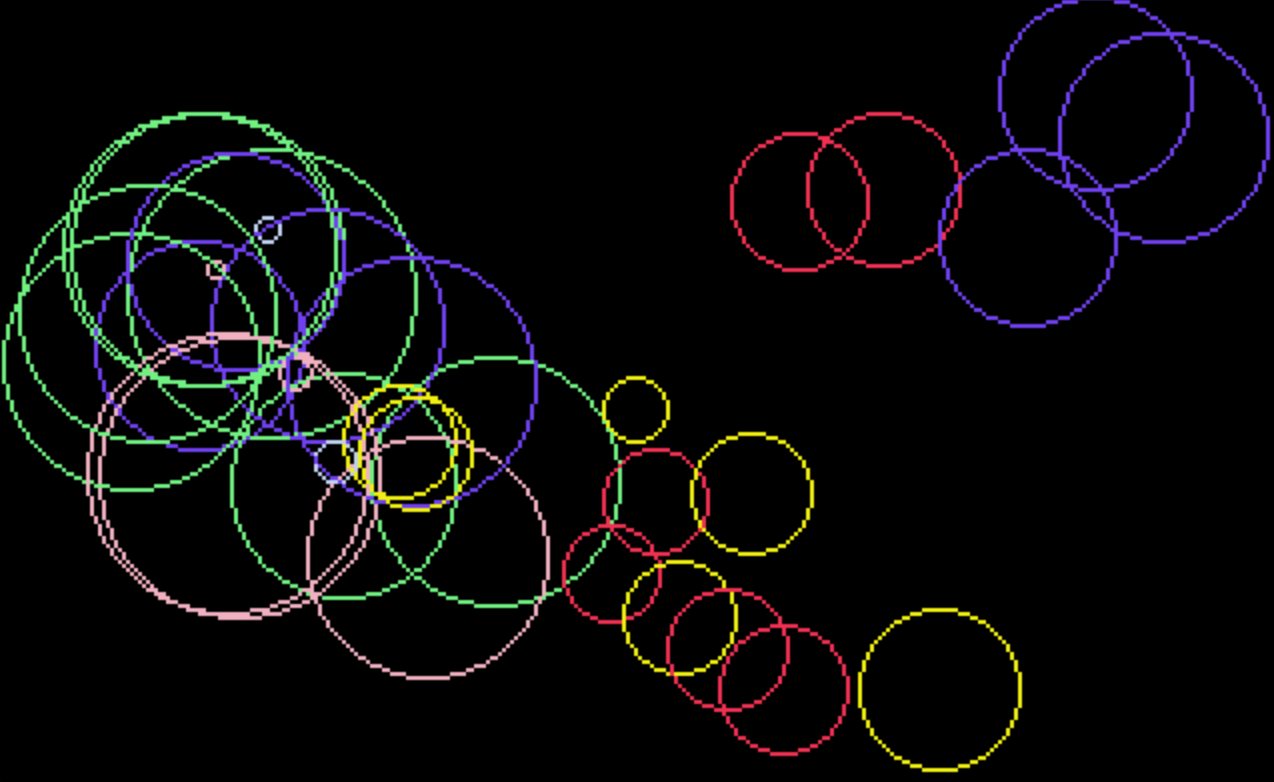
\includegraphics[width=\linewidth]{images/circle.png}\end{center}
\newpage

\item [Example:] Using {\bf CIRCLE}
\begin{tcolorbox}[colback=black,coltext=white]
\verbatimfont{\codefont}
\begin{verbatim}
100 REM CIRCLE (AFTER F.BOWEN)
110 BORDER 0                            :REM BLACK
120 SCREEN 320,200,4                    :REM SIMPLE SCREEN SETUP
130 PALETTE 0,0,0,0,0                   :REM BLACK
140 PALETTE 0,1,RND(.)*16,RND(.)*16,15  :REM RANDOM COLOURS
150 PALETTE 0,2,RND(.)*16,15,RND(.)*16
160 PALETTE 0,3,15,RND(.)*16,RND(.)*16
170 PALETTE 0,4,RND(.)*16,RND(.)*16,15
180 PALETTE 0,5,RND(.)*16,15,RND(.)*16
190 PALETTE 0,6,15,RND(.)*16,RND(.)*16
200 SCNCLR 0                            :REM CLEAR
210 FORI=0TO32                          :REM CIRCLE LOOP
220 PEN 0,RND(.)*6+1                    :REM RANDOM PEN
230 R=RND(.)*36+1                       :REM RADIUS
240 XC=R+RND(.)*320:IF(XC+R)>319THEN240:REM X CENTRE
250 YC=R+RND(.)*200:IF(YC+R)>199THEN250:REM Y CENTRE
260 XC=XC+WT*320:YC=YC+HT*200
270 CIRCLE XC,YC,R,.                    :REM DRAW
280 NEXT
290 GETKEY A$                           :REM WAIT FOR KEY
300 SCREEN CLOSE:BORDER 6
\end{verbatim}
\end{tcolorbox}
\end{description}

% *****
% CLOSE
% *****

\newpage
\subsection{CLOSE}
\index{BASIC 65 Commands!CLOSE}
\begin{description}[leftmargin=2cm,style=nextline]
\item [Token:] \$A0
\item [Format:] {\bf CLOSE} channel
\item [Usage:] Closes an input or output channel.

               {\bf channel} number, which was given to a previous
               call of commands such as {\bf APPEND}, {\bf DOPEN}, or {\bf OPEN}.

\item [Remarks:] Closing files that have previously been opened
               before a program has completed is
               very important, especially for output files.
               {\bf CLOSE} flushes output buffers and
               updates the directory information on disks.
               Failing to {\bf CLOSE} can corrupt files and disks.
               BASIC does NOT automatically close channels nor files
               when a program stops.

\item [Example:] Using {\bf CLOSE}
\begin{tcolorbox}[colback=black,coltext=white]
\verbatimfont{\codefont}
\begin{verbatim}
10 OPEN 2,8,2,"TEST,S,W"
20 PRINT#2,"TESTSTRING"
30 CLOSE 2 : REM OMITTING CLOSE GENERATES A SPLAT FILE
\end{verbatim}
\end{tcolorbox}
\end{description}

% ***
% CLR
% ***

\newpage
\subsection{CLR}
\index{BASIC 65 Commands!CLR}
\begin{description}[leftmargin=2cm,style=nextline]
\item [Token:] \$9C
\item [Format:] {\bf CLR}        \\
                {\bf CLR V}
\item [Usage:] Used for management of BASIC variables, arrays
               and strings. The run-time stack pointers,
               and the table of open channels is reset
               After executing a {\bf CLR} all variables and arrays will be undeclared.
               {\bf RUN} performs {\bf CLR} automatically.

               {\bf CLR V} clears (zeroes) the variable V.
               V can be a numeric variable or a string variable, but not
               an array.

\item [Remarks:] {\bf CLR} should not be used inside loops or
               subroutines, as it destroys the return address.
               After a {\bf CLR}, all variables are unknown and will
               be initialised when they are next used.

\item [Example:] Using {\bf CLR}
\begin{tcolorbox}[colback=black,coltext=white]
\verbatimfont{\codefont}
\begin{verbatim}
10 A=5: P$="MEGA65"
20 CLR
30 PRINT A;P$
RUN

 0
\end{verbatim}
\end{tcolorbox}
\end{description}

% ***
% CMD
% ***

\newpage
\subsection{CMD}
\index{BASIC 65 Commands!CMD}
\begin{description}[leftmargin=2cm,style=nextline]
\item [Token:] \$9D
\item [Format:] {\bf CMD} channel [{\bf,}string]
\item [Usage:] Redirects the standard output
               from screen to a channel. This enables you to
               print listings and directories to other output channels.
               It is also possible to redirect this output to a disk file,
               or a modem.

               {\bf channel} number, which was given to a previous
               call of commands such as {\bf APPEND}, {\bf DOPEN}, or {\bf OPEN}.

               The optional {\bf string} is sent to the channel
               before the redirection begins and can be used,
               for example, for printer or modem setup escape sequences.

\item [Remarks:] The {\bf CMD} mode is stopped by a {\bf PRINT\#},
                 or by closing the channel with {\bf CLOSE}.
                 It is recommended to use {\bf PRINT\#}
                 before closing, to make sure that the output buffer
                 has been flushed.

\item [Example:] Using {\bf CMD} to print a program listing:
\begin{tcolorbox}[colback=black,coltext=white]
\verbatimfont{\codefont}
\begin{verbatim}
OPEN 1,4    :REM OPEN CHANNEL #1 TO PRINTER AT UNIT 4
CMD 1
LIST
PRINT#1
CLOSE 1
\end{verbatim}
\end{tcolorbox}
\end{description}

% *******
% COLLECT
% *******

\newpage
\subsection{COLLECT}
\index{BASIC 65 Commands!COLLECT}
\begin{description}[leftmargin=2cm,style=nextline]
\item [Token:] \$F3
\item [Format:] {\bf COLLECT} [{\bf,D} drive] [{\bf,U} unit]
\item [Usage:]
   Rebuilds the {\bf BAM}
   (Block Availability Map) of a disk, deleting splat files (files which have been opened,
   but not properly closed) and marking unused blocks as free.

   \drivedefinition

   \unitdefinition

\item [Remarks:]
   While this command is useful for cleaning a disk from
   splat files, it is dangerous for disks with boot blocks or random access files.
   These blocks are not associated with standard disk files
   and will therefore be marked as free and may be overwritten
   by further disk write operations.


\item [Examples:] Using {\bf COLLECT}
\begin{tcolorbox}[colback=black,coltext=white]
\verbatimfont{\codefont}
\begin{verbatim}
  COLLECT
  COLLECT U9
  COLLECT D0, U9
\end{verbatim}
\end{tcolorbox}
\end{description}

% *********
% COLLISION
% *********

\newpage
\subsection{COLLISION}
\index{BASIC 65 Commands!COLLISION}
\begin{description}[leftmargin=2cm,style=nextline]
\item [Token:] \$FE \$17
\item [Format:] {\bf COLLISION} type [{\bf,}line number]
\item [Usage:]  Enables or disables
                a user-programmed interrupt handler.
                A call without the linenumber argument disables the handler,
                while a call with linenumber enables it.
                After the execution of {\bf COLLISION} with
                linenumber, a sprite collision of the same type,
                (as specified in the {\bf COLLISION} call)
                interrupts the BASIC program and performs a {\bf GOSUB}
                to {\bf linenumber}, which is expected to contain
                the user code for handling sprite collisions.
                This handler must give control back with a {\bf RETURN}.

                {\bf type} specifies the collision type for
                this interrupt handler:
                    \begin{longtable}{ c | l}
                    1	& 	sprite - sprite collision \\
                    2	& 	sprite - data - collision \\
                    3	& 	light pen \\
                    \end{longtable}

                {\bf linenumber} must point to a subroutine
                which has code for handling sprite collision
                and ends with a {\bf RETURN}.

\item [Remarks:] It is possible to enable the interrupt handler for
               all types, but only one can execute at any time.
               An interrupt handler cannot be interrupted by another
               interrupt handler.
               Functions such as {\bf BUMP}, {\bf RSPPOS} and
               {\bf LPEN} may be used for evaluation of the sprites
               which are involved, and their positions.

\item [Info:] {\bf COLLISION} is one of the commands, which was not
              working in BASIC 10 and needs to be fixed for BASIC 65.
              A new implementation will be available in a future ROM file update.

\item [Example:] Using {\bf COLLISION}
\begin{tcolorbox}[colback=black,coltext=white]
\verbatimfont{\codefont}
\begin{verbatim}
10 COLLISION 1,70 : REM ENABLE
20 SPRITE 1,1 : MOVSPR 1,120,  0 : MOVSPR 1,0#5
30 SPRITE 2,1 : MOVSPR 2,120,100 : MOVSPR 2,180#5
40 FOR I=1 TO 50000:NEXT
50 COLLISION 1 : REM DISABLE
60 END
70 REM SPRITE <-> SPRITE INTERRUPT HANDLER
80 PRINT "BUMP RETURNS";BUMP(1)
90 RETURN: REM RETURN FROM INTERRUPT
\end{verbatim}
\end{tcolorbox}
\end{description}

% *****
% COLOR
% *****

\newpage
\subsection{COLOR}
\index{BASIC 65 Commands!COLOR}
\begin{description}[leftmargin=2cm,style=nextline]
\item [Token:] \$E7
\item [Format:] {\bf COLOR} <{\bf ON} | {\bf OFF}>
\item [Usage:] Enables or disables
               handling of character attributes on screen.
               If {\bf COLOR} is {\bf ON}, the screen routines
               take care of both character RAM and attribute RAM (or colour RAM).
               For example, if the screen is scrolling text, the attributes
               are also scrolled, so each character keeps its attribute.
               If {\bf COLOR} is {\bf OFF}, the attribute
               is fixed and only character movement is performed
               for screen characters. This speeds up screen
               handling, which could be useful when moving characters with different colours is
               not intended.
\item [Example:] \screentext{COLOR ON} - with colour/attribute handling \\
                 \screentext{COLOR OFF} - no colour/attribute handling

\end{description}

% ******
% CONCAT
% ******

\newpage
\subsection{CONCAT}
\index{BASIC 65 Commands!CONCAT}
\begin{description}[leftmargin=2cm,style=nextline]
\item [Token:] \$FE \$13
\item [Format:] {\bf CONCAT} appendfile [{\bf,D} drive] {\bf TO}
                targetfile [{\bf,D} drive] [{\bf,U} unit]
\item [Usage:]
   {\bf CONCAT} (concatenation) appends the contents of
   {\bf appendfile} to the {\bf targetfile}. Afterwards, {\bf targetfile}
   contains the contents of both files, while {\bf appendfile}
   remains unchanged.

   {\bf appendfile} is either a quoted string, for example: {\bf "data"} or
   a string expression in brackets, for example: {\bf (FI\$)}

   {\bf targetfile} is either a quoted string, for example: {\bf "safe"} or
   a string expression in brackets, for example: {\bf (FS\$)}

   If the disk unit has dual drives, it is possible to apply
   {\bf CONCAT} to files which are stored on different
   disks. In this case, it is necessary to specify the drive\#
   for both files. This is also necessary if both
   files are stored on drive\#1.

   \drivedefinition

   \unitdefinition

\item [Remarks:]
   {\bf CONCAT} is executed in the DOS of the disk drive.
   Both files must exist and no pattern matching is allowed.
   Only files of type {\bf SEQ} may be concatenated.

\item [Examples:] Using {\bf CONCAT}
\begin{tcolorbox}[colback=black,coltext=white]
\verbatimfont{\codefont}
\begin{verbatim}
  CONCAT "NEW DATA" TO "ARCHIVE" ,U9
  CONCAT "ADDRESS",D0 TO "ADDRESS BOOK",D1
\end{verbatim}
\end{tcolorbox}
\end{description}

% ****
% CONT
% ****

\newpage
\subsection{CONT}
\index{BASIC 65 Commands!CONT}
\begin{description}[leftmargin=2cm,style=nextline]
\item [Token:] \$9A
\item [Format:] {\bf CONT}
\item [Usage:] Used to resume
               program execution after a break or stop caused by
               an {\bf END} or {\bf STOP} statement, or by pressing
               \specialkey{RUN STOP}.
               This is a useful debugging tool. The BASIC program may be stopped
               and variables can be examined, and even changed.
               The {\bf CONT} statement resumes execution.
\item [Remarks:] {\bf CONT} cannot be used, if a program has stopped because
               of an error. Also ,any editing of a program
               inhibits continuation. Stopping and continuation
               can spoil the screen output, and can also interfere with
               input/output operations.
\item [Example:] Using {\bf CONT}
\begin{tcolorbox}[colback=black,coltext=white]
\verbatimfont{\codefont}
\begin{verbatim}
10 I=I+1:GOTO 10
RUN

BREAK IN 10
READY.
PRINT I
 947
CONT
\end{verbatim}
\end{tcolorbox}
\end{description}

% ****
% COPY
% ****

\newpage
\subsection{COPY}
\index{BASIC 65 Commands!COPY}
\begin{description}[leftmargin=2cm,style=nextline]
\item [Token:] \$F4
\item [Format:] {\bf COPY} source [{\bf,D} drive] [{\bf,U} unit] {\bf TO}
                [target] [{\bf ,D} drive] [{\bf ,U} unit]
\item [Usage:]
   Copies the contents of
   {\bf source} to {\bf target}.
   It is used to copy either single files or, by using
   wildcard characters, multiple files.

   {\bf source} is either a quoted string, e.g. {\bf "data"} or
   a string expression in brackets, e.g. {\bf (FI\$)}.

   {\bf target} is either a quoted string, e.g. {\bf "backup"} or
   a string expression in brackets, e.g. {\bf (FS\$)}

   \drivedefinition

   \unitdefinition

   If none or one unit number is given, or the unit numbers before and after
   the TO token are equal, {\bf COPY} is executed on the disk drive
   itself, and the source and target files will be on the same disk.

   If the source unit (before TO) is different to the target unit (after TO),
   {\bf COPY} is executed in MEGA65 BASIC by reading the source
   files into a RAM buffer and writing to the target unit. In this case,
   the target file name cannot be chosen, it will be the same as the
   source filename. The extended unit-to-unit copy mode allows the copying of
   single files, pattern matching files or all files of a disk.
   Any combination of units is allowed, internal floppy, SD card images,
   IEC floppy drives such as the 1541, 1571, 1581, or CMD floppy and hard drives.

\item [Remarks:]
   The file types {\bf PRG}, {\bf SEQ} and {\bf USR} can be copied.
   If source and target are on the same disk, the target filename
   must be different from the source file name.

   {\bf COPY} cannot copy {\bf DEL} files, that are commonly used
   as titles or separators in disk directories. These do not conform to
   Commodore DOS rules and cannot be accessed by standard {\bf OPEN} routines.

   {\bf REL} files cannot be copied from unit to unit.

\item [Examples:] Using {\bf COPY}
\begin{tcolorbox}[colback=black,coltext=white]
\verbatimfont{\codefont}
\begin{verbatim}
  COPY U8 TO U9            :REM COPY ALL FILES
  COPY "CODES" TO "BACKUP" :REM COPY SINGLE FILE
  COPY "*.TXT",U8 TO U9    :REM PATTERN COPY
  COPY "M*",U9 TO U11      :REM PATTERN COPY
\end{verbatim}
\end{tcolorbox}
\end{description}

% ***
% COS
% ***

\newpage
\subsection{COS}
\index{BASIC 65 Functions!COS}
\begin{description}[leftmargin=2cm,style=nextline]
\item [Token:] \$BE
\item [Format:] {\bf COS(}numeric expression{\bf )}
\item [Usage:] Returns the cosine of the argument.
               The argument is expected in units of {\bf radians}.
               The result is in the range (-1.0 to +1.0)

\item [Remarks:] An argument in units of {\bf degrees}
                 can be converted to {\bf radians}
                 by multiplying it with $\pi/180$.
\item [Examples:] Using {\bf COS}
\begin{tcolorbox}[colback=black,coltext=white]
\verbatimfont{\codefont}
\begin{verbatim}
PRINT COS(0.7)
 0.76484219

X=60:PRINT COS(X * ~ / 180)
 0.5
\end{verbatim}
\end{tcolorbox}
\end{description}

% ******
% CURSOR
% ******

\newpage
\subsection{CURSOR}
\index{BASIC 65 Commands!CURSOR}
\begin{description}[leftmargin=2cm,style=nextline]
%\item [Token:] \$??
\item [Format:] {\bf CURSOR} <{\bf ON} | {\bf OFF}> [\{{\bf,} column{\bf,} row{\bf,} style\}] \\
		{\bf CURSOR} \{column{\bf,} row{\bf,} style\}
\item [Usage:] Moves the text cursor to
               the specified position on the current text screen.

               {\bf ON} or {\bf OFF} displays or hides the cursor.

               {\bf column} and {\bf row} specify the new position.

               {\bf style} defines a solid (1) or flashing (0) cursor.
%\item [Remarks:]
\item [Example:] Using {\bf CURSOR}
\begin{tcolorbox}[colback=black,coltext=white]
\verbatimfont{\codefont}
\begin{verbatim}
10  SCNCLR
20  CURSOR ON,1,2,1         :REM DISPLAY A SOLID CURSOR AT COLUMN 1, ROW 2
30  PRINT "A"; : SLEEP 1
40  CURSOR ,,0              :REM CHANGE TO A FLASHING CURSOR
50  PRINT "B"; : SLEEP 1
60  CURSOR OFF              :REM HIDE THE CURSOR
70  PRINT "C"; : SLEEP 1
80  CURSOR 20,10            :REM MOVE THE CURSOR TO COLUMN 20, ROW 10
90  PRINT "D"; : SLEEP 1
100 CURSOR ,50              :REM MOVE THE CURSOR TO ROW 5 BUT DO NOT CHANGE THE COLUMN
110 PRINT "E"; : SLEEP 1
100 CURSOR 0                :REM MOVE THE CURSOR TO THE START OF THE ROW
110 PRINT "F"; : SLEEP 1
\end{verbatim}
\end{tcolorbox}
\end{description}

% ****
% DATA
% ****

\newpage
\subsection{DATA}
\index{BASIC 65 Commands!DATA}
\begin{description}[leftmargin=2cm,style=nextline]
\item [Token:] \$83
\item [Format:] {\bf DATA} [list of constants]
\item [Usage:] Used to define constants
               which can be read by {\bf READ} statements
               in a program. Numbers and strings are allowed, but expressions are not.
               Items are separated by commas.
               Strings containing commas, colons or spaces must be placed
               in quotes.

               {\bf RUN} initialises the data pointer
               to the first item of the first {\bf DATA} statement
               and advances it for every read item. It is the
               programmer's responsibility that the type of
               the constant and the variable in the {\bf READ}
               statement match. Empty items with no constant
               between commas are allowed and will be interpreted as
               zero for numeric variables and an empty string for
               string variables.

               {\bf RESTORE} may be used to set the
               data pointer to a specific line for subsequent
               reads.

\item [Remarks:] It is good programming practice to put large amounts of
               {\bf DATA} statements at the end of the program,
               so they don't slow down the search for line numbers
               after {\bf GOTO}, and other statements with line number targets.
\item [Example:] Using {\bf DATA}
\begin{tcolorbox}[colback=black,coltext=white]
\verbatimfont{\codefont}
\begin{verbatim}
1 REM DATA
10 READ NA$, VE
20 READ N% : FOR I=2 TO N% : READ GL(I) : NEXT I
30 PRINT "PROGRAM:";NA$;"  VERSION:";VE
40 PRINT "N-POINT GAUSSLEGENDRE FACTORS E1":
50 FOR I=2 TO N%:PRINT I;GL(I):NEXT I
60 END
80 DATA "MEGA65",1.1
90 DATA 5,0.5120,0.3573,0.2760,0.2252

RUN
PROGRAM:MEGA65  VERSION: 1.1
N-POINT GAUSSLEGENDRE FACTORS E1
 2  0.512
 3  0.3573
 4  0.276
 5  0.2252
\end{verbatim}
\end{tcolorbox}
\end{description}

% ******
% DCLEAR
% ******

\newpage
\subsection{DCLEAR}
\index{BASIC 65 Commands!DCLEAR}
\begin{description}[leftmargin=2cm,style=nextline]
\item [Token:] \$FE \$15
\item [Format:] {\bf DCLEAR} [{\bf,D} drive] [{\bf,U} unit]
\item [Usage:]
   Sends an initialise command to the specified unit and drive.

   \drivedefinition

   \unitdefinition

   The DOS of the disk drive will close all open files,
   clear all channels, free buffers and re-read the BAM.
   All open channels on the computer will also be closed.

\item [Examples:] Using {\bf DCLEAR}
\begin{tcolorbox}[colback=black,coltext=white]
\verbatimfont{\codefont}
\begin{verbatim}
  DCLEAR
  DCLEAR U9
  DCLEAR D0, U9
\end{verbatim}
\end{tcolorbox}
\end{description}

% ******
% DCLOSE
% ******

\newpage
\subsection{DCLOSE}
\index{BASIC 65 Commands!DCLOSE}
\begin{description}[leftmargin=2cm,style=nextline]
\item [Token:] \$FE \$0F
\item [Format:] {\bf DCLOSE} [{\bf\#} channel] [{\bf,U} unit]
\item [Usage:]
   Closes a single file or
   all files for the specified unit.

    {\bf channel} number, which was given to a previous
    call to commands such as {\bf APPEND}, {\bf DOPEN}, or {\bf OPEN}.

   \unitdefinition

   {\bf DCLOSE} is used either with a channel argument
   or a unit number, but never both.

\item [Remarks:]
   It is important to close all open files before a program ends.
   Otherwise buffers will not be freed and even worse, open files that have been written to
   may be incomplete (commonly called splat files), and no longer usable.

\item [Examples:] Using {\bf DCLOSE}
\begin{tcolorbox}[colback=black,coltext=white]
\verbatimfont{\codefont}
\begin{verbatim}
  DCLOSE#2 :REM CLOSE FILE ASSIGNED TO CHANNEL 2
  DCLOSE U9:REM CLOSE ALL FILES OPEN ON UNIT 9
\end{verbatim}
\end{tcolorbox}
\end{description}

% ***
% DEC
% ***

\newpage
\subsection{DEC}
\index{BASIC 65 Functions!DEC}
\begin{description}[leftmargin=2cm,style=nextline]
\item [Token:] \$D1
\item [Format:] {\bf DEC(}string expression{\bf)}
\item [Usage:] Returns the decimal value
               of the argument, that is written as a hex string.
               The argument range is "0000" to "FFFF" (0 to 65535 in decimal).
               The argument must have 1-4 hex digits.

\item [Remarks:] Allowed digits in uppercase/graphics mode are: \\
                 0123456789ABCDEF and in lowercase/uppercase mode: \\
                 0123456789abcdef.

\item [Example:] Using {\bf DEC}
\begin{tcolorbox}[colback=black,coltext=white]
\verbatimfont{\codefont}
\begin{verbatim}
  PRINT DEC("D000")
   53248
  POKE DEC("600"),255
\end{verbatim}
\end{tcolorbox}
\end{description}

% ***
% DEF
% ***

\newpage
\subsection{DEF FN}
\index{BASIC 65 Commands!DEF FN}
\index{BASIC 65 Functions!FN}
\begin{description}[leftmargin=2cm,style=nextline]
\item [Token:] \$96
\item [Format:] {\bf DEF FN} name{\bf(}real variable{\bf) =} [expression]
\item [Usage:] Defines a single statement
               user function with one argument of type real,
               returning a real value.
               The definition must be executed before the function
               can be used in expressions. The argument is
               a dummy variable, which will be replaced by the
               argument when the function is used.

\item [Remarks:] The value of the dummy variable will not change
                 and the variable may be used in other contexts
                 without side effects.

\item [Example:] Using {\bf DEF FN}
\begin{tcolorbox}[colback=black,coltext=white]
\verbatimfont{\codefont}
\begin{verbatim}
10 PD = ~ / 180
20 DEF FN CD(X)= COS(X*PD): REM COS FOR DEGREES
30 DEF FN SD(X)= SIN(X*PD): REM SIN FOR DEGREES
40 FOR D=0 TO 360 STEP 90
50 PRINT USING "###";D
60 PRINT USING " ##.##";FNCD(D);
70 PRINT USING " ##.##";FNSD(D)
80 NEXT D
RUN
  0  1.00  0.00
 90  0.00  1.00
180 -1.00  0.00
270  0.00 -1.00
360  1.00  0.00
\end{verbatim}
\end{tcolorbox}
\end{description}

% ******
% DELETE
% ******

\newpage
\subsection{DELETE}
\index{BASIC 65 Commands!DELETE}
\begin{description}[leftmargin=2cm,style=nextline]
\item [Token:] \$F7
\item [Format:] {\bf DELETE} [line range] \\
                {\bf DELETE} filename [{\bf,D} drive] [{\bf,U} unit] [{\bf,R}]
\item [Usage:] Used to either delete
               a range of lines from the BASIC program or to delete file from disk.

               {\bf line range} consists of the first and last
               line to delete, or a single line number.
               If the first number is omitted, the
               first BASIC line is assumed.
               The second number in the range specifier defaults
               to the last BASIC line.

   {\bf filename} is either a quoted string, for example: {\bf "safe"} or
   a string expression in brackets, for example: {\bf (FS\$)}

   \drivedefinition

   \unitdefinition

   {\bf R} Recover a previously deleted file.
   This will only work if there were no write operations
   between deletion and recovery, which may have altered the
   contents of the file.

\item [Remarks:] {\bf DELETE filename} works similar to
                 {\bf SCRATCH filename}.

\item [Examples:] Using {\bf DELETE}
\begin{tcolorbox}[colback=black,coltext=white]
\verbatimfont{\codefont}
\begin{verbatim}
  DELETE 100      :REM DELETE LINE 100
  DELETE 240-350  :REM DELETE ALL LINES FROM 240 TO 350
  DELETE 500-     :REM DELETE FROM 500 TO END
  DELETE -70      :REM DELETE FROM START TO 70

  DELETE "DRM",U9 :REM DELETE FILE DRM ON UNIT 9
\end{verbatim}
\end{tcolorbox}
\end{description}

% ***
% DIM
% ***

\newpage
\subsection{DIM}
\index{BASIC 65 Commands!DIM}
\begin{description}[leftmargin=2cm,style=nextline]
\item [Token:] \$86
\item [Format:] {\bf DIM} name{\bf(}limits{\bf)} [{\bf,} name{\bf(}limits{\bf)} ...]
\item [Usage:] Declares the shape,
               the bounds and the type of a BASIC array.
               As a declaration statement, it must be executed
               only once and before any usage of the declared arrays.
               An array can have one or more dimensions.
               One dimensional arrays are often called vectors
               while two or more dimensions define a matrix.
               The lower bound of a dimension is always zero,
               while the upper bound is declared. The rules for
               variable names apply for array names as well.
               There are integer arrays, real arrays and string arrays.
               It is legal to use the same identifier for scalar
               variables and array variables. The left parenthesis
               after the name identifies array names.

\item [Remarks:] Integer arrays consume two bytes per element,
                 real arrays five bytes and string arrays three bytes
                 for the string descriptor plus
                 the length of the string itself. \\
                 If an array identifier is used without being previously
                 declared, an implicit declaration of an
                 one dimensional array with limit of 10 is performed.

\item [Example:] Using {\bf DIM}
\begin{tcolorbox}[colback=black,coltext=white]
\verbatimfont{\codefont}
\begin{verbatim}
1 REM DIM
10 DIM A%(8)    : REM ARRAY OF 9 ELEMEMTS
20 DIM XX(2,3)  : REM ARRAY OF 3X4 = 12 ELEMENTS
30 FOR I=0 TO 8 : A%(I)=PEEK(256+I) : PRINT A%(I);: NEXT:PRINT
40 FOR I=0 TO 2 : FOR J=0 TO 3 : READ XX(I,J):PRINT XX(I,J);: NEXT J,I
50 END
60 DATA 1,-2,3,-4,5,-6,7,-8,9,-10,11,-12

RUN
 45  52  50  0  0  0  0  0  0
 1 -2  3 -4  5 -6  7 -8  9 -10  11 -12
\end{verbatim}
\end{tcolorbox}
\end{description}

% ***
% DIR
% ***

\newpage
\subsection{DIR}
\index{BASIC 65 Commands!DIR}
\begin{description}[leftmargin=2cm,style=nextline]
\item [Token:] \$EE (DIR) \$FE \$29 (ECTORY)
\item [Format:] {\bf DIR} [filepattern] [{\bf,W}] [{\bf,R}] [{\bf,D} drive] [{\bf,U} unit] \\
		{\bf DIRECTORY} [filepattern] [{\bf,W}] [{\bf,R}] [{\bf,D} drive] [{\bf,U} unit] \\
		{\bf \$} [filepattern] [{\bf,W}] [{\bf,R}] [{\bf,D} drive] [{\bf,U} unit]
\item [Usage:]  Prints a file directory/catalog of the specified disk.

   The {\bf W} (Wide) parameter lists the directory three columns wide
   on the screen and pauses after the screen has been filled with a page
   (63 directory entries). Pressing any key displays the next page.

   The {\bf R} (Recoverable) parameter includes files in the
   directory, which are flagged as deleted but are still
   recoverable.

   {\bf filepattern} is either a quoted string, for example: {\bf "da*"} or
   a string expression in brackets, e.g. {\bf (DI\$)}

   \drivedefinition

   \unitdefinition

\item [Remarks:]
   {\bf DIR} is a synonym for {\bf CATALOG}
   or {\bf DIRECTORY}, and produces the same listing.
   The {\bf filepattern} can be used to filter the listing.
   The wildcard characters {\bf *} and {\bf ?} may be used.
   Adding {\bf ,T=} to the pattern string, with {\bf T} specifying
   a filetype of {\bf P}, {\bf S}, {\bf U} or {\bf R}
   (for {\bf P}RG, {\bf S}EQ, {\bf U}SR, {\bf R}EL) filters the
   output to that filetype.

   The shortcut symbol {\bf \$} can only be used in direct mode.

\item [Examples:] Using {\bf DIR}

% Character test

%\begin{tcolorbox}[colback=black,coltext=white]
%\verbatimfont{\codefont}
%\begin{verbatim}
%
% !"#$%&'()*+,-./
%0123456789:;<=>?
%@ABCDEFGHIJKLMNO
%PQRSTUVWXYZ[\]^_
%`abcdefghijklmno
%pqrstuvwxyz{|}~
%
%ÀÁÂÃÄÅÆÇÈÉÊËÌÍÎÏ
%ÐÑÒÓÔÕÖ×ØÙÚÛÜÝÞß
%àáâãäåæçèéêëìíîï
%ðñòóôõö÷øùúûüýþÿ
%
%ĀāĂ㥹ĆćĈĉĊċČčĎď
%ĐđĒēĔĕĖėĘęĚěĜĝĞğ
%ĠġĢģĤĥĦħĨĩĪīĬĭĮį
%İıIJijĴĵĶķĸĹĺĻļĽľĿ
%
%ŀŁłŃńŅņŇňʼnŊŋŌōŎŏ
%ŐőŒœŔŕŖŗŘřŚśŜŝŞş
%ŠšŢţŤťŦŧŨũŪūŬŭŮů
%ŰűŲųŴŵŶŷŸŹźŻżŽžſ
%
%\end{verbatim}
%\end{tcolorbox}

\begin{tcolorbox}[colback=black,coltext=white]
\verbatimfont{\codefont}
\begin{verbatim}
DIR
\end{verbatim}
\selectfont{\codefont 0}
\begin{tcolorbox}[colback=white,coltext=black,arc=0mm,boxrule=0mm,
       left*=0.5mm,right*=0mm,top=0mm,bottom=0mm,nobeforeafter,
       left skip=0.5mm,
       width=28mm,height=3mm,valign=center]
\begin{verbatim}
"BLACK SMURF     " BS 2A
\end{verbatim}
\end{tcolorbox}
\begin{verbatim}
508  "STORY PHOBOS"     SEQ
27   "C8096"            PRG
25   "C128"             PRG
104 BLOCKS FREE.
\end{verbatim}
\end{tcolorbox}

For a {\bf DIR} listing with the {\bf w}ide parameter, please refer to the example under {\bf CATALOG}
on page \pageref{3columndirlisting}.
%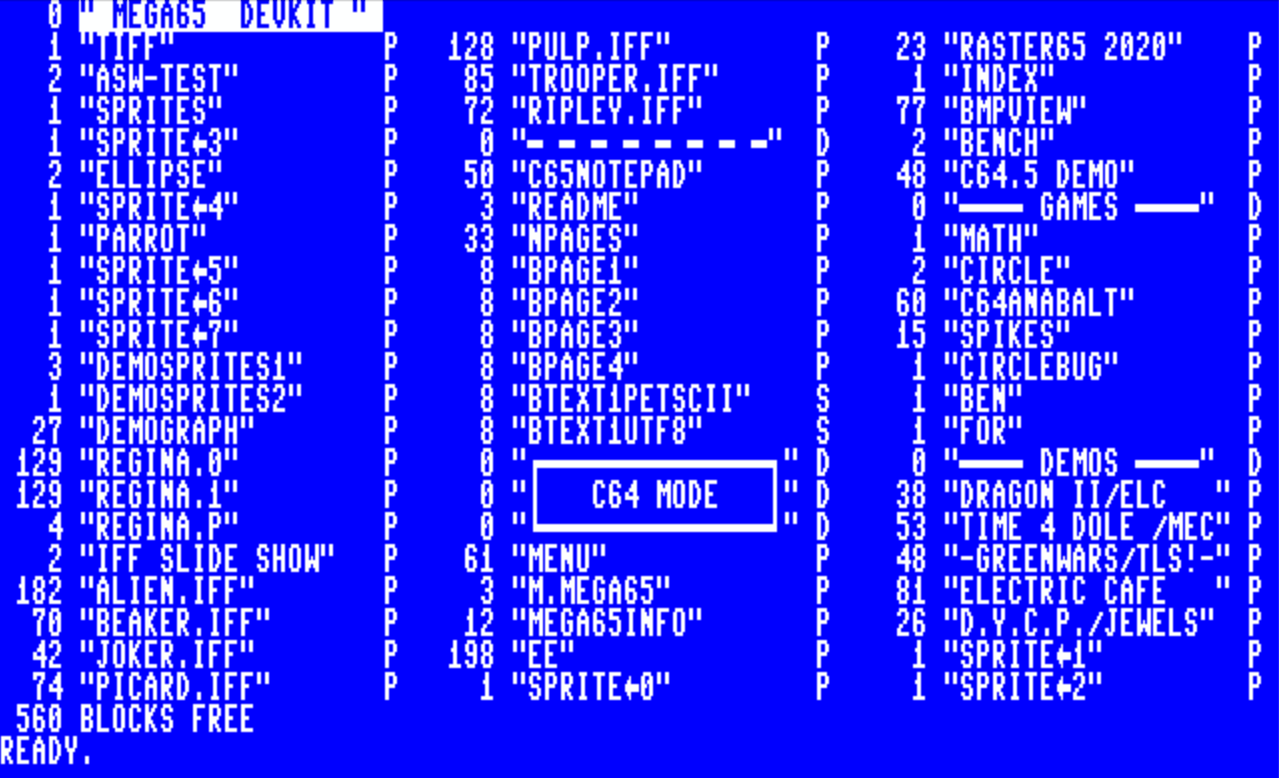
\includegraphics[width=\linewidth]{images/directory.png}

\end{description}

% ****
% DISK
% ****

\newpage
\subsection{DISK}
\index{BASIC 65 Commands!DISK}
\begin{description}[leftmargin=2cm,style=nextline]
\item [Token:] \$FE \$40
\item [Format:] {\bf DISK} command [{\bf,U} unit] \\
		{\bf @} command [{\bf,U} unit]
\item [Usage:]

   Sends a command string to the specified disk unit.

   \unitdefinition

   {\bf command} is a string expression.

\item [Remarks:]
   The command string is interpreted by the disk unit
   and must be compatible to the used DOS version.
   Read the disk drive manual for possible commands.

   Using {\bf DISK} with no parameters prints the disk status.

   The shortcut symbol {\bf @} can only be used in direct mode.

\item [Examples:] Using {\bf DISK}
\begin{tcolorbox}[colback=black,coltext=white]
\verbatimfont{\codefont}
\begin{verbatim}
  DISK "I0"   :REM INITIALISE DISK IN DRIVE 0
  DISK "U0>9" :REM CHANGE UNIT# TO 9
\end{verbatim}
\end{tcolorbox}
\end{description}

% *****
% DLOAD
% *****

\newpage
\subsection{DLOAD}
\index{BASIC 65 Commands!DLOAD}
\begin{description}[leftmargin=2cm,style=nextline]
\item [Token:] \$F0
\item [Format:] {\bf DLOAD} filename [{\bf,D} drive] [{\bf,U} unit]
\item [Usage:]
   "Disk LOAD" loads a file of type
   {\bf PRG} into memory reserved for BASIC programs.

   \filenamedefinition

   \drivedefinition

   \unitdefinition

\item [Remarks:]
   The load address, which is stored in the first two bytes
   of the file is ignored. The program is loaded into
   BASIC memory. This enables loading of BASIC programs
   that were saved on other computers with different memory
   configurations. After loading, the program is re-linked
   and ready to be run or edited.
   It is possible to use {\bf DLOAD} in a running program. This is
   called overlaying, or chaining.
   If you do this, then the newly loaded program replaces the current one,
   and the execution starts automatically on the first line of the
   new program. Variables, arrays and strings from the current
   run are preserved and can also be used by the newly loaded program.

\item [Examples:] Using {\bf DLOAD}
\begin{tcolorbox}[colback=black,coltext=white]
\verbatimfont{\codefont}
\begin{verbatim}
  DLOAD "APOCALYPSE"
  DLOAD "MEGA TOOLS",U9
  DLOAD (FI$),U(UN%)
\end{verbatim}
\end{tcolorbox}
\end{description}

% ***
% DMA
% ***

\newpage
\subsection{DMA}
\label{BASIC 65 Commands!DMA}
\index{BASIC 65 Commands!DMA}
\begin{description}[leftmargin=2cm,style=nextline]
\item [Token:] \$FE \$1F
\item [Format:] {\bf DMA} command [{\bf,} length{\bf,} source address{\bf,}
                 source bank{\bf,} target address{\bf,} target bank
                 [{\bf,} sub]]
\item [Usage:]
   {\bf DMA} ("Direct Memory Access") is obsolete,
   and has been replaced by {\bf EDMA}.

   {\bf command} 0 = copy, 1 = mix, 2 = swap, 3 = fill

   {\bf length} number of bytes

   {\bf source address} = 16-bit address of read area or fill byte

   {\bf source bank} bank number for source (ignored for fill mode)

   {\bf target} = 16-bit address of write area

   {\bf target bank} bank number for target

   {\bf sub} sub command

\item [Remarks:]
{\bf DMA} has access to the lower 1MB address range
organised in 16 banks of 64 K. To avoid this limitation, use
{\bf EDMA}, which has access to the full 256MB address range.

\item [Examples:] A sequence of {\bf DMA} calls to demonstrate fast screen drawing operations
\begin{tcolorbox}[colback=black,coltext=white]
\verbatimfont{\codefont}
\begin{verbatim}
DMA 0, 80*25, 2048, 0, 0, 4  :REM SAVE SCREEN TO $00000 BANK 4
DMA 3, 80*25, 32, 0, 2048, 0 :REM FILL SCREEN WITH BLANKS
DMA 0, 80*25, 0, 4, 2048, 0  :REM RESTORE SCREEN FROM $00000 BANK 4
DMA 2, 80, 2048, 0, 2048+80, 0 :REM SWAP CONTENTS OF LINE 1 & 2 OF SCREEN
\end{verbatim}
\end{tcolorbox}
\end{description}

% *****
% DMODE
% *****

\newpage
\subsection{DMODE}
\index{BASIC 65 Commands!DMODE}
\begin{description}[leftmargin=2cm,style=nextline]
\item [Token:] \$FE \$35
\item [Format:] {\bf DMODE} jam{\bf,} complement{\bf,} inverse{\bf,}
		stencil{\bf,} style{\bf,} thick
\item [Usage:]
   "Display MODE" sets several parameters of the graphics context, which is used by drawing commands.

\begin{center}
\ttfamily
\begin{tabular}{|l|l|}
\hline
   {\bf jam}        &  0 - 1 \\
   {\bf complement} &  0 - 1 \\
   {\bf inverse}    &  0 - 1 \\
   {\bf stencil}    &  0 - 1 \\
   {\bf style}      &  0 - 3 \\
   {\bf thick}      &  1 - 8 \\
\hline
\end{tabular}
\end{center}
\end{description}

% **
% DO
% **

\newpage
\subsection{DO}
\index{BASIC 65 Commands!DO}
\begin{description}[leftmargin=2cm,style=nextline]
\item [Token:] \$EB
\item [Format:] {\bf DO} ... {\bf LOOP} \\
                {\bf DO} [<{\bf UNTIL} | {\bf WHILE}> logical expression] \\
                . . . statements [{\bf EXIT}] \\
                {\bf LOOP} [<{\bf UNTIL} | {\bf WHILE}> logical expression]
\item [Usage:] {\bf DO} and {\bf LOOP} define
               the start of a BASIC loop.
               Using {\bf DO} and {\bf LOOP} alone without any
               modifiers creates an infinite loop, which can only be exited
               by the {\bf EXIT} statement. The loop can be
               controlled by adding {\bf UNTIL} or {\bf WHILE}
               after the {\bf DO} or {\bf LOOP}.

\item [Remarks:] {\bf DO} loops may be nested. An {\bf EXIT} statement
               only exits the current loop.
\item [Examples:] Using {\bf DO} and {\bf LOOP}
\begin{tcolorbox}[colback=black,coltext=white]
\verbatimfont{\codefont}
\begin{verbatim}
10 PW$="":DO
20 GET A$:PW$=PW$+A$
30 LOOP UNTIL LEN(PW$)>7 OR A$=CHR$(13)

10 DO : REM WAIT FOR USER DECISION
20 GET A$
30 LOOP UNTIL A$="Y" OR A$="N" OR A$="y" OR A$="n"

10 DO WHILE ABS(EPS) > 0.001
20 GOSUB 2000 : REM ITERATION SUBROUTINE
30 LOOP

10 I%=0 : REM INTEGER LOOP 1-100
20 DO I%=I%+1
30 LOOP WHILE I% < 101
\end{verbatim}
\end{tcolorbox}
\end{description}

% *****
% DOPEN
% *****

\newpage
\subsection{DOPEN}
\begin{description}[leftmargin=2cm,style=nextline]
\item [Token:] \$FE \$0D
\item [Format:] {\bf DOPEN\#} channel{\bf,} filename
		[{\bf,L} [reclen]] [{\bf,W}] [{\bf,D} drive] [{\bf,U} unit]
\item [Usage:]
    Opens a file for reading or writing.

    {\bf channel} number, where:
    \begin{itemize}
        \item {\bf 1 <= channel <= 127} line terminator is CR.
        \item {\bf 128 <= channel <= 255} line terminator is CR LF.
    \end{itemize}

   {\bf L} indicates, that the file is a relative file, which
   is opened for read/write, as well as random access. The reclength
   is mandatory for creating relative files. For existing
   relative files, the {\bf reclen} is used as a safety check, if given.

   {\bf W} opens a file for write access. The file must not exist.

   \filenamedefinition

   \drivedefinition

   \unitdefinition

\item [Remarks:]
   {\bf DOPEN\#} may be used to open all file types.
   The sequential file type {\bf SEQ} is default.
   The relative file type {\bf REL} is chosen by using the
   {\bf L} parameter.  Other file types
   must be specified in the filename, e.g. by adding ",P" to the
   filename for {\bf PRG} files or ",U" for {\bf USR} files.

   If the first character of the filename is an at sign '@', it
   is interpreted as a "save and replace" operation. It is not recommended
   to use this option on 1541 and 1571 drives, as they
   contain a "save and replace bug" in their DOS.

\newpage
\item [Examples:] Using {\bf DOPEN}

\begin{tcolorbox}[colback=black,coltext=white]
\verbatimfont{\codefont}
\begin{verbatim}
   DOPEN#5,"DATA",U9
   DOPEN#130,(DD$),U(UN%)
   DOPEN#3,"USER FILE,U"
   DOPEN#2,"DATA BASE",L240
   DOPEN#4,"MYPROG,P" : REM OPEN PRG FILE
\end{verbatim}
\end{tcolorbox}
\end{description}

% ****
% DPAT
% ****

\newpage
\subsection{DPAT}
\index{BASIC 65 Commands!DPAT}
\begin{description}[leftmargin=2cm,style=nextline]
\item [Token:] \$FE \$36
\item [Format:] {\bf DPAT} type [{\bf,} number{\bf,} pattern ...]
\item [Usage:]
   "Drawing PATtern" sets the pattern
   of the graphics context for drawing commands.

\begin{center}
\ttfamily
\begin{tabular}{|l|l|}
\hline
   {\bf type}       &  0-63 \\
   {\bf number}     &  1-4 \\
   {\bf pattern}    &  0-255 \\
\hline
\end{tabular}
\end{center}
\end{description}

% **
% DS
% **

\newpage
\subsection{DS}
\index{BASIC 65 System Variables!DS}
\begin{description}[leftmargin=2cm,style=nextline]
\item [Format:] {\bf DS}
\item [Usage:]  {\bf DS} holds the status of the last disk operation.
                It is a volatile variable.
                Each use triggers the reading of the disk status
                from the current disk device in usage.
                {\bf DS} is coupled to the string variable {\bf DS\$}
                which is updated at the same time.
                Reading the disk status from a disk device automatically
                clears any error status on that device, so subsequent reads
                will return 0, if no other activity was in between.
\item[Remarks:] {\bf DS} is a reserved system variable.

\item [Example:] Using {\bf DS}
\begin{tcolorbox}[colback=black,coltext=white]
\verbatimfont{\codefont}
\begin{verbatim}
100 DOPEN#1,"DATA"
110 IF DS<>0 THEN PRINT"COULD NOT OPEN FILE DATA":STOP
\end{verbatim}
\end{tcolorbox}
\end{description}

% ****
% DS\$
% ****

\newpage
\subsection{DS\$}
\index{BASIC 65 System Variables!DS\$}
\begin{description}[leftmargin=2cm,style=nextline]
\item [Format:] {\bf DS\$}
\item [Usage:]  {\bf DS\$} holds the status of the last disk operation
                in text form of the format:
                Code,Message,Track,Sector.

                {\bf DS\$} is coupled to the numeric variable {\bf DS}
                It is updated when {\bf DS} is used.
                DS\$ is set to "00,OK,00,00", if there was no error, otherwise
                it is set to a DOS error message (listed in the
                disk manuals).
\item[Remarks:] {\bf DS\$} is a reserved system variable.

\item [Example:] Using {\bf DS\$}
\begin{tcolorbox}[colback=black,coltext=white]
\verbatimfont{\codefont}
\begin{verbatim}
100 DOPEN#1,"DATA"
110 IF DS<>0 THEN PRINT DS$:STOP
\end{verbatim}
\end{tcolorbox}
\end{description}

% *****
% DSAVE
% *****

\newpage
\subsection{DSAVE}
\index{BASIC 65 Commands!DSAVE}
\begin{description}[leftmargin=2cm,style=nextline]
\item [Token:] \$EF
\item [Format:] {\bf DSAVE} filename [{\bf,D} drive] [{\bf,U} unit]
\item [Usage:]
   "Disk SAVE" saves the BASIC program to
   a file of type {\bf PRG}.

   \filenamedefinition
   The maximum length of the filename is 16 characters.
   If the first character of the filename is an at sign '@' it
   is interpreted as a "save and replace" operation. It is not recommended
   to use this option on 1541 and 1571 drives, as they
   contain a "save and replace bug" in their DOS.

   \drivedefinition

   \unitdefinition

\item [Remarks:]
   The {\bf DVERIFY} can be used after {\bf DSAVE} to check,
   if the saved program on disk is identical to the program
   in memory.

\item [Example:] Using {\bf DSAVE}
\begin{tcolorbox}[colback=black,coltext=white]
\verbatimfont{\codefont}
\begin{verbatim}
  DSAVE "ADVENTURE"
  DSAVE "ZORK-I",U9
  DSAVE "DUNGEON",D1,U10
\end{verbatim}
\end{tcolorbox}
\end{description}

% ****
% DT\$
% ****

\newpage
\subsection{DT\$}
\index{BASIC 65 System Variables!DT\$}
\begin{description}[leftmargin=2cm,style=nextline]
\item [Format:] {\bf DT\$}
\item [Usage:]  {\bf DT\$} holds the current date and is updated before
                each usage from the RTC (Real-Time Clock).
                The RTC can be set in the Configure Menu.
                The string {\bf DT\$} is formatted as:
                "DD-MON-YYYY", for example: "04-APR-2021".
\item[Remarks:] {\bf DT\$} is a reserved system variable.

\item [Example:] Using {\bf DT\$}
\begin{tcolorbox}[colback=black,coltext=white]
\verbatimfont{\codefont}
\begin{verbatim}
100 PRINT "TODAY IS: ";DT$
\end{verbatim}
\end{tcolorbox}
\end{description}

% *******
% DVERIFY
% *******

\newpage
\subsection{DVERIFY}
\index{BASIC 65 Commands!DVERIFY}
\begin{description}[leftmargin=2cm,style=nextline]
\item [Token:] \$FE \$14
\item [Format:] {\bf DVERIFY} filename [{\bf,D} drive] [{\bf,U} unit]
\item [Usage:]
   "Disk VERIFY" compares the BASIC program
   in memory with a disk file of type {\bf PRG}.

   \filenamedefinition

   \drivedefinition

   \unitdefinition

\item [Remarks:]
   {\bf DVERIFY} can only test for equality. It gives no information
   about the number or position of different valued bytes.
    {\bf DVERIFY} exits either with the message \screentext{OK}
    or with \screentext{VERIFY ERROR}.

\item [Example:] Using {\bf DVERIFY}
\begin{tcolorbox}[colback=black,coltext=white]
\verbatimfont{\codefont}
\begin{verbatim}
  DVERIFY "ADVENTURE"
  DVERIFY "ZORK-I",U9
  DVERIFY "DUNGEON",D1,U10
\end{verbatim}
\end{tcolorbox}
\end{description}

% ****
% EDIT
% ****

\newpage
\subsection{EDIT}
\index{BASIC 65 System Commands!EDIT}
\begin{description}[leftmargin=2cm,style=nextline]
\item [Format:] {\bf EDIT} <{\bf ON} | {\bf OFF}>

\item [Usage:]  {\bf EDIT} switches the builtin editor
               either to text mode {\bf EDIT ON}
               or BASIC program editor {\bf EDIT OFF}.

               After power up or reset, the editor
               is initialised as BASIC program editor.

               After setting the editor to text mode with
               {\bf EDIT ON}, the diffences to program mode are:

               The editor does no tokenising/parsing.
               All text entered after a linenumber remains pure text,
               BASIC keywords such as {\bf FOR} and {\bf GOTO} are not
               converted to BASIC tokens, as they are whilst in program mode.

               The line numbers are only used for text organisation,
               sorting, deleting, listing etc.
               When the text is saved to file with {\bf DSAVE},
               a sequential file (type {\bf SEQ}) is written, not a
               program ({\bf PRG}) file, which is what happens whilst in program mode.
               Line numbers are not written to the file.

               {\bf DLOAD} in text mode can load only sequential files.
               Line numbers are automatically generated for editing purposes.

               The mode of the editor can be recognised by looking at the prompt:
               In program mode, the prompt is: {\bf READY.}, whilst in text mode
               the prompt is: {\bf OK}.

               The text mode affects entered lines with leading number only,
               lines with no linenumber are executed as BASIC commands,
               as usual.

               Sequential files, created with the text editor, can be displayed
               (without loading them)
               on the screen by using {\bf TYPE <filename>}.

\newpage

\item [Example:] Using {\bf EDIT}
\begin{tcolorbox}[colback=black,coltext=white]
\verbatimfont{\codefont}
\begin{verbatim}
ready.
edit on

ok.
100 This is a simple text editor.
dsave "example"

ok.
new

ok.
catalog

0 "demoempty       " 00 3d
1    "example"          seq
3159 blocks free

ok.
type "example"
This is a simple text editor.

ok.
dload "example"

loading

ok.
list

1000 This is a simple text editor.

ok.
\end{verbatim}
\end{tcolorbox}
\end{description}

% ****
% EDMA
% ****

\newpage
\subsection{EDMA}
\label{BASIC 65 Commands!EDMA}
\index{BASIC 65 Commands!EDMA}
\begin{description}[leftmargin=2cm,style=nextline]
\item [Token:] \$FE \$21
\item [Format:] {\bf EDMA} command{\bf,} length{\bf,} source{\bf,}
                 target [{\bf,} sub{\bf,} mod]
\item [Usage:]
   {\bf EDMA} ("Extended Direct Memory Access") is the fastest method
   to manipulate memory areas using the DMA controller.

   {\bf command} 0 = copy, 1 = mix, 2 = swap, 3 = fill.

   {\bf length} number of bytes (maximum = 65535).

   {\bf source}  28-bit address of read area or fill byte.

   {\bf target} 28-bit address of write area.

   {\bf sub} sub command (see chapter on DMA controller).

   {\bf mod} modifier (see chapter on DMA controller).

\item [Remarks:]
{\bf EDMA} can access the entire 256MB address range,
using up to 28 bits for the addresses of the source and target.
\item [Examples:] Using {\bf EDMA}
\begin{tcolorbox}[colback=black,coltext=white]
\verbatimfont{\codefont}
\begin{verbatim}
EDMA 0, $800, $F700, $8000000 :REM COPY SCALAR VARIABLES TO ATTIC RAM
EDMA 3, 80*25, 32, 2048       :REM FILL SCREEN WITH BLANKS
EDMA 0, 80*25, 2048, $8000800 :REM COPY SCREEN TO ATTIC RAM
\end{verbatim}
\end{tcolorbox}
\end{description}

% **
% EL
% **

\newpage
\subsection{EL}
\index{BASIC 65 System Variables!EL}
\begin{description}[leftmargin=2cm,style=nextline]
\item [Format:] {\bf EL}
\item [Usage:]  {\bf EL} has the value of the line where
               the most recent BASIC error occurred,
                or the value -1 if there was no error.
\item [Remarks:] {\bf EL} is a reserved system variable.

This variable is typically used in a TRAP routine,
where the error line is taken from {\bf EL}.

\item [Example:] Using {\bf EL}
\begin{tcolorbox}[colback=black,coltext=white]
\verbatimfont{\codefont}
\begin{verbatim}
 10 TRAP 100
 20 PRINT SQR(-1)     :REM PROVOKE ERROR
 30 PRINT "AT LINE 30":REM HERE TO RESUME
 40 END
100 IF ER>0 THEN PRINT ERR$(ER);" ERROR"
110 PRINT " IN LINE";EL
120 RESUME NEXT       :REM RESUME AFTER ERROR
\end{verbatim}
\end{tcolorbox}
\end{description}

% *******
% ELLIPSE
% *******

\newpage
\subsection{ELLIPSE}
\index{BASIC 65 Commands!ELLIPSE}
\begin{description}[leftmargin=2cm,style=nextline]
\item [Token:] \$FE \$30
\item [Format:] {\bf ELLIPSE} xcentre{\bf,} ycentre{\bf,} xradius{\bf,} yradius
		[{\bf,} solid]
\item [Usage:] Draws an ellipse.

               {\bf xcentre} x coordinate of centre in pixels.

               {\bf ycentre} y coordinate of centre in pixels.

               {\bf xradius} x radius of the ellipse in pixels.

               {\bf yradius} y radius of the ellipse in pixels.

               {\bf solid} fills the ellipse, if not zero.

\item [Remarks:] {\bf ELLIPSE} is used to draw ellipses on
               screens at various resolutions.
               It can also be used to draw circles.

\item [Example:] Using {\bf ELLIPSE}


\item \begin{center}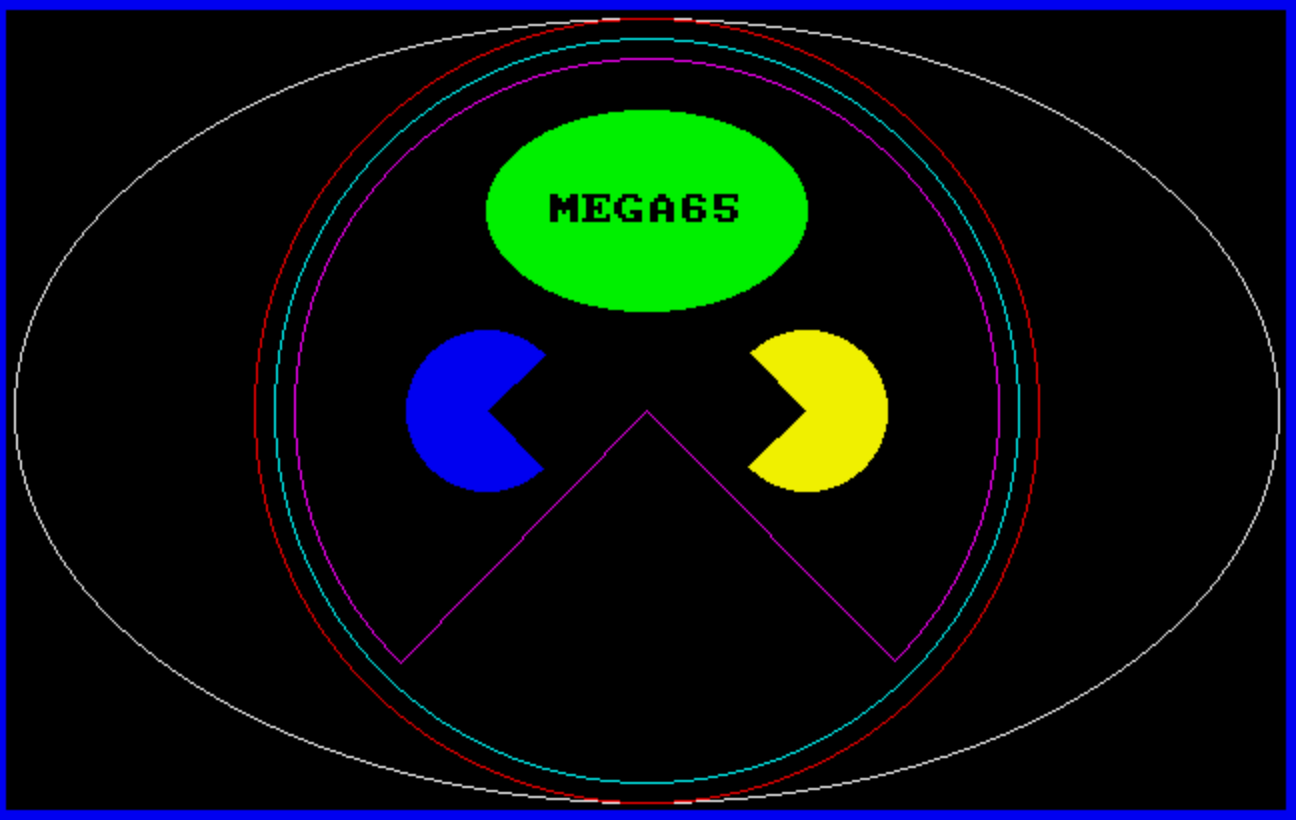
\includegraphics[width=0.7\linewidth]{images/ellipse.png}\end{center}

\newpage
\begin{tcolorbox}[colback=black,coltext=white]
\verbatimfont{\codefont}
\begin{verbatim}
100 REM ELLIPSE
110 W=320:H=200:B%=2            :REM WIDTH, HEIGHT, DEPTH
120 X0=W/2:Y0=H/2:XD=W/4:YD=H/4 :REM CENTRE AND HALF AXIS
130 BORDER 0                    :REM BLACK
140 BACKGROUND 0                :REM BLACK
150 FOREGROUND 5                :REM GREEN
160 SCREEN 320,200,B%           :REM SET PARAMETERS
170 PEN 2                       :REM DRAW PEN RED
180 ELLIPSE X0,Y0,XD,YD,1       :REM DRAW SOLID ELLIPSE
190 PEN 3                       :REM DRAW PEN CYAN
200 ELLIPSE X0,Y0,XD+8,YD+8,0   :REM DRAW OUTLINED ELLIPSE
210 A$=STR$(W)+" X"+STR$(H)+" X"+STR$(B%)
220 PEN 1                       :REM DRAW PEN WHITE
230 CHAR  12,10,1,1,2,A$        :REM DRAW TEXT
240 GETKEY A$                   :REM WWAIT FOR KEYPRESS
250 SCREEN CLOSE                :REM CLOSE GRAPHICS
\end{verbatim}
\end{tcolorbox}
\end{description}
% ****
% ELSE
% ****

\newpage
\subsection{ELSE}
\index{BASIC 65 Commands!ELSE}
\begin{description}[leftmargin=2cm,style=nextline]
\item [Token:] \$D5
\item [Format:] {\bf IF} expression {\bf THEN} true clause
		{\bf ELSE} false clause
\item [Usage:] {\bf ELSE} is part of an {\bf IF}
               statement.

               {\bf expression} a logical or numeric expression.
               A numeric expression is evaluated as {\bf FALSE}
               if the value is zero and {\bf TRUE} for any non-zero
               value.

               {\bf true clause} one or more statements starting
               directly after {\bf THEN} on the same line.
               A line number after {\bf THEN} performs a
               {\bf GOTO} to that line instead.

               {\bf false clause} one or more statements starting
               directly after {\bf ELSE} on the same line.
               A linenumber after {\bf ELSE} performs a
               {\bf GOTO} to that line instead.

\item [Remarks:]
               The standard {\bf IF ... THEN ... ELSE} structure
               is restricted to a single line. But the {\bf true clause}
               or {\bf false clause} may be expanded to several lines
               using a compound statement surrounded with
               {\bf BEGIN} and {\bf BEND}.
\item [Example:]
                Using {\bf ELSE}
\begin{tcolorbox}[colback=black,coltext=white]
\verbatimfont{\codefont}
\begin{verbatim}
100 REM ELSE
110 RED$=CHR$(28):BLACK$=CHR$(144):WHITE$=CHR$(5)
120 INPUT "ENTER A NUMBER";V
130 IF V<0 THENPRINT RED$;:ELSEPRINT BLACK$;
140 PRINT V : REM PRINT NEGATIVE NUMBERS IN RED
150 PRINT WHITE$
160 INPUT "END PROGRAM:(Y/N)";A$
170 IF A$="Y" THENEND
180 IF A$="N" THEN120:ELSE160
\end{verbatim}
\end{tcolorbox}
\end{description}


% ***
% END
% ***

\newpage
\subsection{END}
\index{BASIC 65 Commands!END}
\begin{description}[leftmargin=2cm,style=nextline]
\item [Token:] \$80
\item [Format:] {\bf END}
\item [Usage:] Ends the execution
               of the BASIC program. The {\bf READY.} prompt
               appears and the computer goes into direct mode
               waiting for keyboard input.

\item [Remarks:]
               {\bf END} does {\bf not} clear channels nor close files.
               Also, variable definitions are still valid after {\bf END}.
               The program may be continued with the {\bf CONT}
               statement. After executing the last line of a
               program, {\bf END} is automatically executed.


\item [Example:]
                Using {\bf END}
\begin{tcolorbox}[colback=black,coltext=white]
\verbatimfont{\codefont}
\begin{verbatim}
10 IF V < 0 THEN END : REM NEGATIVE NUMBERS END THE PROGRAM
20 PRINT V
\end{verbatim}
\end{tcolorbox}
\end{description}

% ********
% ENVELOPE
% ********

\newpage
\subsection{ENVELOPE}
\index{BASIC 65 Commands!ENVELOPE}
\begin{description}[leftmargin=2cm,style=nextline]
\item [Token:] \$FE \$0A
\item [Format:] {\bf ENVELOPE} n [\{{\bf,} attack{\bf,} decay{\bf,}
		sustain{\bf,} release{\bf,} waveform{\bf,} pw\}]
\item [Usage:] Used to define
               the parameters for the synthesis of a musical
               instrument.

      {\bf n} envelope slot (0-9).

      {\bf attack} attack rate (0-15).

      {\bf decay} decay rate (0-15).

      {\bf sustain} sustain rate (0-15).

      {\bf release} release rate (0-15).

      {\bf waveform} 0:triangle, 1:sawtooth, 2:square/pulse, 3:noise, 4:ring modulation.

      {\bf pw} pulse width (0-4095) for waveform.

\label{envelopetable}
               There are 10 slots for storing instrument parameters,
               preset with following values:
\begin{center}
\ttfamily
{\setlength{\tabcolsep}{1mm}
\begin{tabular}{*{6}{|R{5mm}}|R{9mm}|l|}
\hline
 n  & A & D  & S  & R  & WF & PW     & Instrument \\
\hline
  0 & 0 &  9 &  0 &  0 &  2 &  1536  &     piano \\
  1 & 12&  0 & 12 &  0 &  1 &        &     accordion \\
  2 & 0 &  0 & 15 &  0 &  0 &        &     calliope \\
  3 & 0 &  5 &  5 &  0 &  3 &        &     drum \\
  4 & 9 &  4 &  4 &  0 &  0 &        &     flute \\
  5 & 0 &  9 &  2 &  1 &  1 &        &     guitar \\
  6 & 0 &  9 &  0 &  0 &  2 &  512   &     harpsichord \\
  7 & 0 &  9 &  9 &  0 &  2 &  2048  &     organ \\
  8 & 8 &  9 &  4 &  1 &  2 &  512   &     trumpet \\
  9 & 0 &  9 &  0 &  0 &  0 &        &     xylophone \\
\hline
\end{tabular}
}
\end{center}
\item [Example:]
                Using {\bf ENVELOPE}
\begin{tcolorbox}[colback=black,coltext=white]
\verbatimfont{\codefont}
\begin{verbatim}
10 ENVELOPE 9,10,5,10,5,2,4000
20 VOL 9
30 TEMPO 30
40 PLAY "T9O4Q CDEFGAB U3T8 CDEFGAB L","T5O3Q H CGEQG T7 HCGEQG L"
\end{verbatim}
\end{tcolorbox}
\end{description}

% *****
% ERASE
% *****

\newpage
\subsection{ERASE}
\index{BASIC 65 Commands!ERASE}
\label{erasecommand}
\begin{description}[leftmargin=2cm,style=nextline]
\item [Token:] \$FE \$2A
\item [Format:] {\bf ERASE} filename [{\bf,D} drive] [{\bf,U} unit] [{\bf,R}]
\item [Usage:] Used
               to erase a disk file.

   \filenamedefinition

   \drivedefinition

   \unitdefinition

   {\bf R} Recover a previously erased file.
   This will only work if there were no write operations
   between erasing and recovery, which may have altered the
   contents of the file.

\item [Remarks:] {\bf ERASE filename} works similarly to {\bf SCRATCH filename}.

                 The success and the number of erased files can
                 be examined by printing or using the system
                 variable {\bf DS\$}. The second to last number from {\bf DS\$}
                 contains the number of successfully erased files,
                 (normally the second to last number in {\bf DS\$}
                 contains the track number in case of a disk error).

\item [Examples:] Using {\bf ERASE}
\begin{tcolorbox}[colback=black,coltext=white]
\verbatimfont{\codefont}
\begin{verbatim}
  ERASE "DRM",U9 :REM ERASE FILE DRM ON UNIT 9
  PRINT DS$
  01, FILES SCRATCHED,01,00
  ERASE "OLD*"   :REM ERASE ALL FILES BEGINNING WITH "OLD"
  PRINT DS$
  01, FILES SCRATCHED,04,00
\end{verbatim}
\end{tcolorbox}
\end{description}

% **
% ER
% **

\newpage
\subsection{ER}
\index{BASIC 65 System Variables!ER}
\begin{description}[leftmargin=2cm,style=nextline]
\item [Format:] {\bf ER}
\item [Usage:]  {\bf ER} has the value of the most recent BASIC error that has
               occurred, or -1 if there was no error.
\item [Remarks:] {\bf ER} is a reserved system variable.

This variable is typically used in a TRAP routine,
where the error number is taken from {\bf ER}.

\item [Example:] Using {\bf ER}
\begin{tcolorbox}[colback=black,coltext=white]
\verbatimfont{\codefont}
\begin{verbatim}
 10 TRAP 100
 20 PRINT SQR(-1)     :REM PROVOKE ERROR
 30 PRINT "AT LINE 30":REM HERE TO RESUME
 40 END
100 IF ER>0 THEN PRINT ERR$(ER);" ERROR"
110 PRINT " IN LINE";EL
120 RESUME NEXT       :REM RESUME AFTER ERROR
\end{verbatim}
\end{tcolorbox}
\end{description}

% *****
% ERR\$
% *****

\newpage
\subsection{ERR\$}
\index{BASIC 65 Functions!ERR\$}
\begin{description}[leftmargin=2cm,style=nextline]
\item [Token:] \$D3
\item [Format:] {\bf ERR\$(}number{\bf)}
\item [Usage:] Used to convert
               an error number to an error string.

   {\bf number} is a BASIC error number (1-41).

This function is typically used in a TRAP routine,
where the error number is taken from the reserved variable {\bf ER}.

\item [Remarks:] Arguments out of range (1-41) will
                 produce an ILLEGAL QUANTITY error.

\item [Example:] Using {\bf ERR\$}
\begin{tcolorbox}[colback=black,coltext=white]
\verbatimfont{\codefont}
\begin{verbatim}
 10 TRAP 100
 20 PRINT SQR(-1)     :REM PROVOKE ERROR
 30 PRINT "AT LINE 30":REM HERE TO RESUME
 40 END
100 IF ER>0 THEN PRINT ERR$(ER);" ERROR"
110 PRINT " IN LINE";EL
120 RESUME NEXT       :REM RESUME AFTER ERROR
\end{verbatim}
\end{tcolorbox}
\end{description}

% ****
% EXIT
% ****

\newpage
\subsection{EXIT}
\index{BASIC 65 Commands!EXIT}
\begin{description}[leftmargin=2cm,style=nextline]
\item [Token:] \$FD
\item [Format:] {\bf EXIT}
\item [Usage:] Exits the current {\bf DO .. LOOP}
               and continues execution at the first
               statement after {\bf LOOP}.

\item [Remarks:] In nested loops, {\bf EXIT} exits only the current loop,
               and continues execution in an outer loop (if there is one).
\item [Example:] Using {\bf EXIT}
\begin{tcolorbox}[colback=black,coltext=white]
\verbatimfont{\codefont}
\begin{verbatim}
1 REM EXIT
10 OPEN 2,8,0,"$"            : REM OPEN CATALOG
15 IF DS THEN PRINT DS$: STOP: REM CANT READ
20 GET#2,D$,D$               : REM DISCARD LOAD ADDRESS
25 DO                        : REM LINE LOOP
30   GET#2,D$,D$             : REM DISCARD LINE LINK
35   IF ST THEN EXIT         : REM END-OF-FILE
40   GET#2,LO,HI             : REM FILE SIZE BYTES
45   S=LO + 256 * HI         : REM FILE SIZE
50   LINE INPUT#2, F$        : REM FILE NAME
55   PRINT S;F$              : REM PRINT FILE ENTRY
60 LOOP
65 CLOSE 2
\end{verbatim}
\end{tcolorbox}
\end{description}

% ***
% EXP
% ***

\newpage
\subsection{EXP}
\index{BASIC 65 Functions!EXP}
\begin{description}[leftmargin=2cm,style=nextline]
\item [Token:] \$BD
\item [Format:] {\bf EXP(}numeric expression{\bf)}
\item [Usage:] The {\bf EXP} (EXPonential function) computes
               the value of the mathematical constant
               Euler's number ({\bf 2.71828183})
               raised to the power of the
               argument.

\item [Remarks:] An argument greater than 88 produces
                 an OVERFLOW ERROR:
\item [Examples:] Using {\bf EXP}
\begin{tcolorbox}[colback=black,coltext=white]
\verbatimfont{\codefont}
\begin{verbatim}
PRINT EXP(1)
 2.71828183

PRINT EXP(0)
 1

PRINT EXP(LOG(2))
 2
\end{verbatim}
\end{tcolorbox}
\end{description}

% ****
% FAST
% ****

\newpage
\subsection{FAST}
\index{BASIC 65 Commands!FAST}
\begin{description}[leftmargin=2cm,style=nextline]
\item [Token:] \$FE \$25
\item [Format:] {\bf FAST} [speed]
\item [Usage:] Set CPU clock to 1MHz, 3.5MHz or 40MHz.

                {\bf speed} CPU clock speed where:
                \begin{itemize}
                    \item {\bf 1} sets CPU to 1MHz.
                    \item {\bf 3} sets CPU to 3MHz.
                    \item Anything other than {\bf 1} or {\bf 3} sets the CPU to 40MHz.
                \end{itemize}
\item [Remarks:] Although it's possible to call {\bf FAST}
                 with any real number, the precision part (the decimal point
                 and any digits after it), will be ignored.

                 {\bf FAST} is a synonym of {\bf SPEED}.

                 {\bf FAST} has no effect if {\bf POKE 0,65}
                 has previously been used to set the CPU to 40MHz.

\item [Example:] Using {\bf FAST}
\begin{tcolorbox}[colback=black,coltext=white]
\verbatimfont{\codefont}
\begin{verbatim}
10 FAST      :REM SET SPEED TO MAXIMUM (40 MHZ)
20 FAST 1    :REM SET SPEED TO 1 MHZ
30 FAST 3    :REM SET SPEED TO 3.5 MHZ
40 FAST 3.5  :REM SET SPEED TO 3.5 MHZ
\end{verbatim}
\end{tcolorbox}
\end{description}

% ******
% FGOSUB
% ******

\newpage
\subsection{FGOSUB}
\index{BASIC 65 Commands!FGOSUB}
\begin{description}[leftmargin=2cm,style=nextline]
\item [Token:] \$FE \$48
\item [Format:] {\bf FGOSUB} numeric expression
\item [Usage:] Evaluates the given numeric expression, then calls ({\bf GOSUB}s) the subroutine at the resulting line number.

\item [Warning:] Using this feature can break your program if {\bf RENUMBER}
is applied, as line numbers may change and the
numeric expression will no longer address your intended line numbers.

\item [Example:] Using {\bf FGOSUB}:
\begin{tcolorbox}[colback=black,coltext=white]
\verbatimfont{\codefont}
\begin{verbatim}
 10 INPUT "WHICH SUBROUTINE TO EXECUTE 100,200,300";LI
 20 FGOSUB LI     :REM HOPEFULLY THIS LINE # EXISTS
 30 GOTO 10       :REM REPEAT
100 PRINT "AT LINE 100":RETURN
200 PRINT "AT LINE 200":RETURN
300 PRINT "AT LINE 300":RETURN
\end{verbatim}
\end{tcolorbox}
\end{description}

% *****
% FGOTO
% *****

\newpage
\subsection{FGOTO}
\index{BASIC 65 Commands!FGOTO}
\begin{description}[leftmargin=2cm,style=nextline]
\item [Token:] \$FE \$47
\item [Format:] {\bf FGOTO} numeric expression
\item [Usage:] Evaluates the given numeric expression, then jumps ({\bf GO}es{\bf TO}) to the resulting line number.

\item [Warning:] Using this feature can break your program if {\bf RENUMBER}
                 is applied, as line numbers may change and the
                 numeric expression will no longer address your intended line numbers.

\item [Example:] Using {\bf FGOTO}:
\begin{tcolorbox}[colback=black,coltext=white]
\verbatimfont{\codefont}
\begin{verbatim}
 10 INPUT "WHICH LINE # TO EXECUTE 100,200,300";LI
 20 FGOTO LI     :REM HOPEFULLY THIS LINE # EXISTS
 30 END
100 PRINT "AT LINE 100":END
200 PRINT "AT LINE 200":END
300 PRINT "AT LINE 300":END
\end{verbatim}
\end{tcolorbox}
\end{description}


% ******
% FILTER
% ******

\newpage
\subsection{FILTER}
\index{BASIC 65 Commands!FILTER}
\begin{description}[leftmargin=2cm,style=nextline]
\item [Token:] \$FE \$03
\item [Format:] {\bf FILTER} sid [\{{\bf,} freq{\bf,} lp{\bf,} bp{\bf,}
		hp{\bf,} res\}]
\item [Usage:] Sets the parameters for a SID sound filter.

      {\bf sid} 1 : right SID, 2 : left SID

      {\bf freq} filter cut off frequency (0 -> 2047)

      {\bf lp} low pass filter (0:off, 1:on)

      {\bf bp} band pass filter (0:off, 1:on)

      {\bf hp} high pass filter (0:off, 1:on)

      {\bf resonance} resonance (0 -> 15)

\item [Remarks:] Missing parameters keep their current value.
                 The effective filter is the sum of
                 of all filter settings.
                 This enables band reject and notch effects.

\item [Example:]
                Using {\bf FILTER}
\begin{tcolorbox}[colback=black,coltext=white]
\verbatimfont{\codefont}
\begin{verbatim}
10 PLAY "T7X1O3P9C"
15 SLEEP 0.02
20 PRINT "LOW PASS SWEEP" :L=1:B=0:H=0:GOSUB 100
30 PRINT "BAND PASS SWEEP":L=0:B=1:H=0:GOSUB 100
40 PRINT "HIGH PASS SWEEP":L=0:B=0:H=1:GOSUB 100
50 GOTO 20
100 REM *** SWEEP ***
110 FOR F = 50 TO 1950 STEP 50
120 IF F >= 1000 THEN FF = 2000-F : ELSE FF = F
130 FILTER 1,FF,L,B,H,15
140 PLAY "X1"
150 SLEEP 0.02
160 NEXT F
170 RETURN
\end{verbatim}
\end{tcolorbox}
\end{description}

% ****
% FIND
% ****

\newpage
\subsection{FIND}
\index{BASIC 65 Commands!FIND}
\begin{description}[leftmargin=2cm,style=nextline]
\item [Token:] \$FE \$2B
\item [Format:] {\bf FIND /}string{\bf/} [{\bf,} line range] \\
		{\bf FIND "}string{\bf"} [{\bf,} line range]
\item [Usage:]  {\bf FIND} is an editor command that can only be used
                in direct mode. It searches a given line range
                (if specified), otherwise the entire BASIC program is searched.
                At each occurrence of the "find string" the line is
                listed with the string highlighted.
                \specialkey{NO\\SCROLL} can be used to pause the output.

\item [Remarks:] Any un-shifted character that is not part of
                 the string can be used instead of {\bf /}.

                 However, using double quotes {\bf "} as a delimiter has a special effect:
                 The search text is not tokenised.
                 {\bf FIND "FOR"} will search for the three letters F, O, and R, not
                 the BASIC keyword {\bf FOR}. Therefore, it can find the word
                 {\bf FOR} in string constants or REM statements, but not
                 in program code.

                 On the other hand, {\bf FIND /FOR/} will find all occurrences of
                 the BASIC keyword, but not the text "FOR" in strings.

                 Partial keywords cannot be searched. For example,
                 {\bf FIND /LOO/} will not find the keyword {\bf LOOP},


\item [Example:] Using {\bf FIND}
\item \begin{center}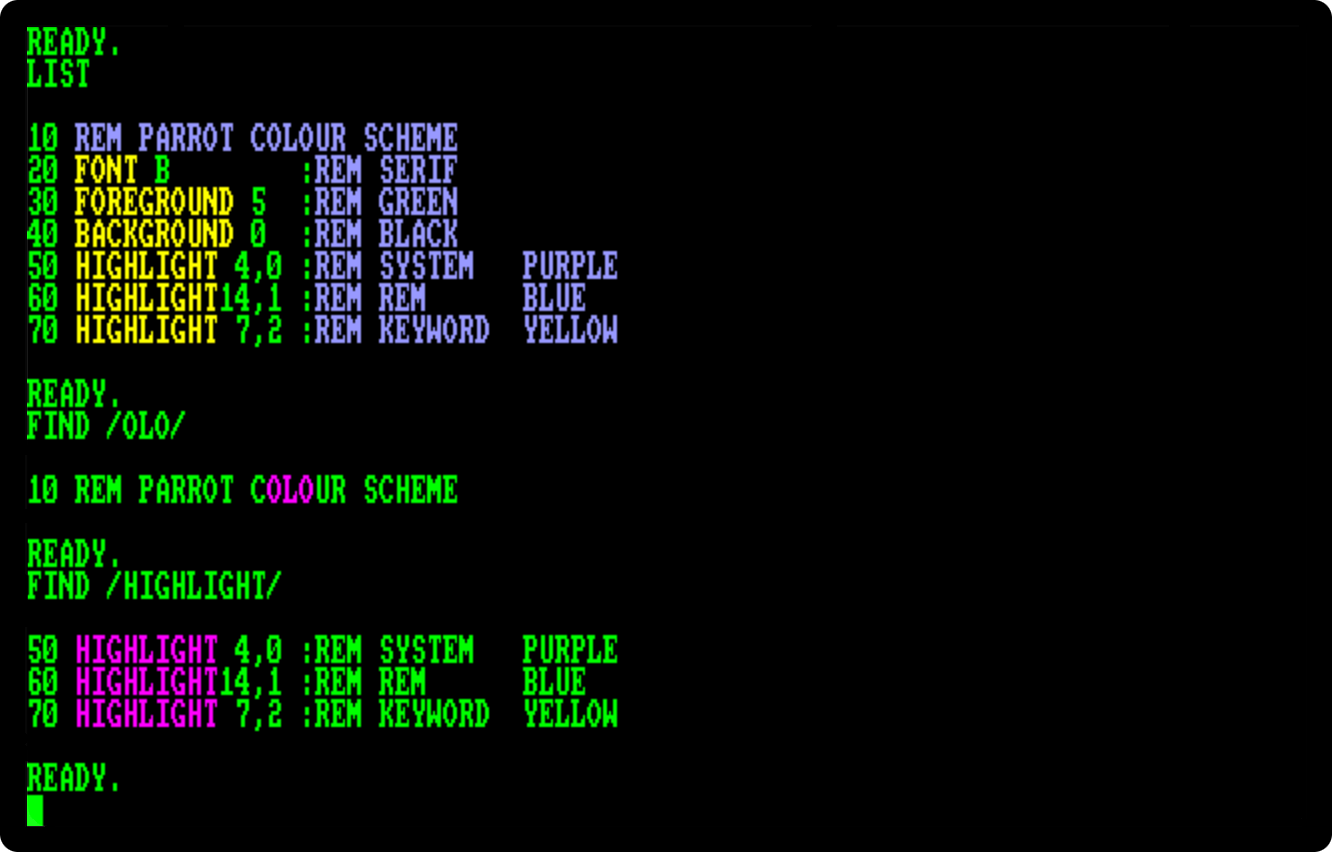
\includegraphics[width=0.8\linewidth]{images/find-example.png}\end{center}
\end{description}

% **
% FN
% **

\newpage
\subsection{FN}
\index{BASIC 65 Functions!FN}
\begin{description}[leftmargin=2cm,style=nextline]
\item [Token:] \$A5
\item [Format:] {\bf FN} name{\bf(}numeric expression{\bf)}
\item [Usage:] {\bf FN} functions are user-defined
               functions, that accept a numeric expression as an
               argument and return a real value.
               They must first be defined with {\bf DEF FN} before
               being used.

\item [Example:] Using {\bf FN}
\begin{tcolorbox}[colback=black,coltext=white]
\verbatimfont{\codefont}
\begin{verbatim}
10 PD = ~ / 180
20 DEF FN CD(X)= COS(X*PD): REM COS FOR DEGREES
30 DEF FN SD(X)= SIN(X*PD): REM SIN FOR DEGREES
40 FOR D=0 TO 360 STEP 90
50 PRINT USING "###";D
60 PRINT USING " ##.##";FNCD(D);
70 PRINT USING " ##.##";FNSD(D)
80 NEXT D
RUN
  0  1.00  0.00
 90  0.00  1.00
180 -1.00  0.00
270  0.00 -1.00
360  1.00  0.00
\end{verbatim}
\end{tcolorbox}
\end{description}

% ****
% FONT
% ****

\newpage
\subsection{FONT}
\index{BASIC 65 Commands!FONT}
\begin{description}[leftmargin=2cm,style=nextline]
\item [Token:] \$FE \$46
\item [Format:] {\bf FONT} <{\bf A} | {\bf B} | {\bf C}>
\item [Usage:] {\bf FONT} is used to switch between fonts,
               and the code pages PETSCII, and enhanced PETSCII.
               The enhanced PETSCII includes all ASCII symbols that
               are missing in the PETSCII code page, although the order
               is still PETSCII.
               The ASCII symbols are typed by holding the \megasymbolkey
               together with the desired key.
               The codes for uppercase and lowercase
               are swapped compared to ASCII.
               The uppercase/graphics code page is not changed.
\begin{center}
\ttfamily
{\setlength{\tabcolsep}{1mm}
\begin{tabular}{*{4}{|R{2.0cm}}|}
\hline
 code  &   key & PETSCII & ASCII  \\
\hline
\$5C & pound      & {\codefont \textbackslash}   & \textbackslash  \\
\$5E & up arrow   & {\codefont \textasciicircum} & \textasciicircum  \\
\$5F & back arrow & {\codefont \_}               & \_   \\
\$7B & colon      & {\codefont ě }               & \{   \\
\$7C & dot        & {\codefont Ĝ }               &  |   \\
\$7D & semicolon  & {\codefont ĝ }               & \}   \\
\$7E & comma      & {\codefont \textasciitilde}  & \textasciitilde   \\
\hline
\end{tabular}
}
\end{center}

% \verbatimfont{\codefont}
% \begin{verbatim}
%  !"#$%&'()*+,-./    20
% 0123456789:;<=>?    30
% @ABCDEFGHIJKLMNO    40
% PQRSTUVWXYZ[\]^_    50
% `abcdefghijklmno    60
% pqrstuvwxyz{|}~     70
%
% ÀÁÂÃÄÅÆÇÈÉÊËÌÍÎÏ  c380
% ÐÑÒÓÔÕÖ×ØÙÚÛÜÝÞß  c390
% àáâãäåæçèéêëìíîï  c3a0
% ðñòóôõö÷øùúûüýþÿ  c3b0
%
% ĀāĂ㥹ĆćĈĉĊċČčĎď  c480
% ĐđĒēĔĕĖėĘęĚěĜĝĞğ  c490
% ĠġĢģĤĥĦħĨĩĪīĬĭĮį  c4a0
% İıIJijĴĵĶķĸĹĺĻļĽľĿ  c4b0
% ŀŁłŃńŅņŇňʼnŊŋŌōŎŏ  c580
% ŐőŒœŔŕŖŗŘřŚśŜŝŞş  c590
%
% ŠšŢţŤťŦŧŨũŪūŬŭŮů  c5a0
% ŰűŲųŴŵŶŷŸŹźŻżŽžſ  c5b0
% ƀƁƂƃƄƅƆƇƈƉƊƋƌƍƎƏ  c680
% ƐƑƒƓƔƕƖƗƘƙƚƛƜƝƞƟ  c690
% \end{verbatim}


\item [Examples:] Using {\bf FONT}
\begin{tcolorbox}[colback=black,coltext=white]
%\verbatimfont{\codefont}
\begin{verbatim}
FONT A :REM ASCII - ENABLE {|}_~^
FONT B :REM LIKE A, WITH A SERIF FONT
FONT C :REM COMMODORE FONT (DEFAULT)
\end{verbatim}
\end{tcolorbox}
\end{description}

% ***
% FOR
% ***

\newpage
\subsection{FOR}
\index{BASIC 65 Commands!FOR}
\begin{description}[leftmargin=2cm,style=nextline]
\item [Token:] \$81
\item [Format:] {\bf FOR} index {\bf=} start {\bf TO} end
		[{\bf STEP} step] ... {\bf NEXT} [index]
\item [Usage:] {\bf FOR} statements start the definition
               of a BASIC loop with an index variable.

               {\bf index} may be incremented or decremented
               by a constant value on each iteration. The default
               is to increment the variable by 1.
               The index variable must be a real variable.

               {\bf start} is used to initialise the index.

               {\bf end} is checked at the end of an iteration,
               and determines whether another iteration will be performed,
               or if the loop will exit.

               {\bf step} defines the change applied to
               to the index variable at the end of an iteration.
               Positive step values increment it, while negative values
               decrement it. It defaults to 1.0 if not specified.

\item [Remarks:] For positive increments {\bf end} must be greater than
               or equal to {\bf start}, whereas for negative increments
               {\bf end} must be less than or equal to {\bf start}.

               It is bad programming practice to change the value
               of the {\bf index} variable inside the loop or to
               jump into or out of a loop body with {\bf GOTO}.

\item [Examples:] Using {\bf FOR}
\begin{tcolorbox}[colback=black,coltext=white]
\verbatimfont{\codefont}
\begin{verbatim}
10 FOR D=0 TO 360 STEP 30
20 R = D * ~ / 180
30 PRINT D;R;SIN(R);COS(R);TAN(R)
40 NEXT D

10 DIM M(20,20)
20 FOR I=0 TO 20
30 FOR J=I TO 20
40 M(I,J) = I + 100 * J
50 NEXT J,I
\end{verbatim}
\end{tcolorbox}
\end{description}

% **********
% FOREGROUND
% **********

\newpage
\subsection{FOREGROUND}
\index{BASIC 65 Commands!FOREGROUND}
\begin{description}[leftmargin=2cm,style=nextline]
\item [Token:] \$FE \$39
\item [Format:] {\bf FOREGROUND} colour
\item [Usage:] Sets the foreground colour
               (text colour) of the screen to the argument,
               which must be in the
               range of 0 to 31.
               Refer to the table under
               {\bf BACKGROUND} on page \pageref{colourtable}
               for the {\bf colour} values and their corresponding colours.

\item [Example:] Using {\bf FOREGROUND}
\item \begin{center}
\includegraphics[width=0.7\linewidth]{images/foreground-example.png}\end{center}
\end{description}

% ***
% FRE
% ***

\newpage
\subsection{FRE}
\index{BASIC 65 Functions!FRE}
\begin{description}[leftmargin=2cm,style=nextline]
\item [Token:] \$B8
\item [Format:] {\bf FRE(}bank{\bf)}
\item [Usage:] Returns the number of free bytes for banks 0 or 1,
               or the ROM version if the argument is negative.

               {\bf FRE(0)} returns the number of free bytes in
               bank 0, which is used for BASIC program source.

               {\bf FRE(1)} returns the number of free bytes in
               bank 1, which is the bank for BASIC variables, arrays
               and strings. {\bf FRE(1)} also triggers
               "garbage collection", which is a process that collects
               used strings at the top of the bank, thereby
               defragmenting string memory.

               {\bf FRE(-1)} returns the ROM version, a six-digit number
               of the form 92xxxx.

\item [Example:] Using {\bf FRE}:
\begin{tcolorbox}[colback=black,coltext=white]
\verbatimfont{\codefont}
\begin{verbatim}
10 PM = FRE(0)
20 VM = FRE(1)
30 RV = FRE(-1)
40 PRINT PM;" FREE FOR PROGRAM"
50 PRINT VM;" FREE FOR VARIABLES"
60 PRINT RV;" ROM VERSION"
\end{verbatim}
\end{tcolorbox}
\end{description}

% *****
% FREAD
% *****

\newpage
\subsection{FREAD}
\index{BASIC 65 Functions!FREAD}
\begin{description}[leftmargin=2cm,style=nextline]
\item [Token:] \$FE \$1C
\item [Format:] {\bf FREAD\#} channel{\bf,} pointer{\bf,} size
\item [Usage:] Reads {\bf size} bytes from {\bf channel} to memory
               starting at the 32-bit address {\bf pointer}.

               {\bf channel} number, which was given to a previous
               call to commands such as {\bf DOPEN}, or {\bf OPEN}.


               Care must be taken not to overwrite memory
               that is used by the system or the interpreter.

               It is recommended to use the {\bf POINTER} statement
               for the pointer argument, and to compute the size parameter
               by multiplying the number of elements with the item size.
\begin{center}
\label{freadtable}
{\ttfamily
\setlength{\tabcolsep}{1mm}
\begin{tabular}{|l|l|}
\hline
 type          & item size \\
\hline
byte     array &  1     \\
integer  array &  2     \\
real     array &  5     \\
\hline
\end{tabular}
}
\end{center}

Keep in mind that the {\bf POINTER} function with a string argument
does NOT return the string address, but the string descriptor.
It is not recommended to use {\bf FREAD} for strings or string arrays
unless you are fully aware on how to handle the string storage internals.

Also, ensure that you always specify an index if you use an array.
The start address of array XY() is POINTER(XY(0)).
POINTER(XY) returns the address of the scalar variable XY.

\item [Example:] Using {\bf FREAD}:
\begin{tcolorbox}[colback=black,coltext=white]
\verbatimfont{\codefont}
\begin{verbatim}
100 N=23
110 DIM B&(N),C&(N)
120 DOPEN#2,"TEXT"
130 FREAD#2,POINTER(B&(0)),N
140 DCLOSE#2
150 FORI=0TON-1:PRINTCHR$(B&(I));:NEXT
160 FORI=0TON-1:C&(I)=B&(N-1-I):NEXT
170 DOPEN#2,"REVERS",W
180 FWRITE#2,POINTER(C&(0)),N
190 DCLOSE#2
\end{verbatim}
\end{tcolorbox}
\end{description}

% *****
% FWRITE
% *****

\newpage
\subsection{FWRITE}
\index{BASIC 65 Functions!FWRITE}
\begin{description}[leftmargin=2cm,style=nextline]
\item [Token:] \$FE \$1E
\item [Format:] {\bf FWRITE\#} channel{\bf,} pointer{\bf,} size
\item [Usage:] Writes {\bf size} bytes to {\bf channel} from memory
               starting at the 32-bit address {\bf pointer}.

               {\bf channel} number, which was given to a previous
               call to commands such as {\bf APPEND}, {\bf DOPEN}, or {\bf OPEN}.

               It is recommended to use the {\bf POINTER} statement
               for the pointer argument and compute the size parameter
               by multiplying the number of elements with the item size.

               Refer to the {\bf FREAD} item size table on page \pageref{freadtable}
               for the item sizes.

Keep in mind that the {\bf POINTER} function with a string argument
does NOT return the string address, but the string descriptor.
It is not recommended to use {\bf FWRITE} for strings or string arrays
unless you are fully aware on how to handle the string storage internals.


Also ensure that you always specify an index if you use an array.
The start address of array XY() is POINTER(XY(0)).
POINTER(XY) returns the address of the scalar variable XY.


\item [Example:] Using {\bf FWRITE}:
\begin{tcolorbox}[colback=black,coltext=white]
\verbatimfont{\codefont}
\begin{verbatim}
100 N=23
110 DIM B&(N),C&(N)
120 DOPEN#2,"TEXT"
130 FREAD#2,POINTER(B&(0)),N
140 DCLOSE#2
150 FORI=0TON-1:PRINTCHR$(B&(I));:NEXT
160 FORI=0TON-1:C&(I)=B&(N-1-I):NEXT
170 DOPEN#2,"REVERS",W
180 FWRITE#2,POINTER(C&(0)),N
190 DCLOSE#2
\end{verbatim}
\end{tcolorbox}
\end{description}

% ***
% GET
% ***

\newpage
\subsection{GET}
\index{BASIC 65 Commands!GET}
\begin{description}[leftmargin=2cm,style=nextline]
\item [Token:] \$A1
\item [Format:] {\bf GET} variable
\item [Usage:] Gets the next character (or byte value of the next character)
               from the keyboard queue.
               If the variable being set to the character is of type string and the queue is empty,
               an empty string is assigned to it,
               otherwise a one character string is created
               and assigned instead.
               If the variable is of type numeric, the byte value
               of the key is assigned to it, otherwise zero will be assigned if the queue is empty.
               {\bf GET} does not wait for keyboard
               input, so it's useful to check for key presses
               at regular intervals or in loops.

\item [Remarks:] {\bf GETKEY} is similar, but waits
                 until a key has been pressed.

\item [Example:] Using {\bf GET}:
\begin{tcolorbox}[colback=black,coltext=white]
\verbatimfont{\codefont}
\begin{verbatim}
10 DO: GET A$: LOOP UNTIL A$ <> ""
40 IF A$ = "W" THEN 1000 :REM GO NORTH
50 IF A$ = "A" THEN 2000 :REM GO WEST
60 IF A$ = "S" THEN 3000 :REM GO EAST
70 IF A$ = "Z" THEN 4000 :REM GO SOUTH
80 IF A$ = CHR$(13) THEN 5000 :REM RETURN
90 GOTO 10
\end{verbatim}
\end{tcolorbox}
\end{description}

% ****
% GET#
% ****

\newpage
\subsection{GET\#}
\index{BASIC 65 Commands!GET\#}
\begin{description}[leftmargin=2cm,style=nextline]
\item [Token:] \$A1 '\#'
\item [Format:] {\bf GET\#} channel{\bf,} variable [{\bf,} variable \dots]
\item [Usage:] Reads as many bytes
               as necessary from the channel argument
               and assigns strings of length one to
               string variables, or an 8-bit binary value
               to numeric variables.
               This is useful for reading characters (or bytes) from
               an input stream one byte at a time.

               {\bf channel} number, which was given to a previous
               call to commands such as {\bf DOPEN}, or {\bf OPEN}.


\item [Remarks:] All values from 0 to 255 are valid, so {\bf GET}
                 can also be used to read binary data.

\item [Example:] Using {\bf GET\#} to read a disk directory:
\begin{tcolorbox}[colback=black,coltext=white]
\verbatimfont{\codefont}
\begin{verbatim}
1 REM GET#
10 OPEN 2,8,0,"$"            : REM OPEN CATALOG
15 IF DS THEN PRINT DS$: STOP: REM CANT READ
20 GET#2,D$,D$               : REM DISCARD LOAD ADDRESS
25 DO                        : REM LINE LOOP
30   GET#2,D$,D$             : REM DISCARD LINE LINK
35   IF ST THEN EXIT         : REM END-OF-FILE
40   GET#2,LO,HI             : REM FILE SIZE BYTES
45   S=LO + 256 * HI         : REM FILE SIZE
50   LINE INPUT#2, F$        : REM FILE NAME
55   PRINT S;F$              : REM PRINT FILE ENTRY
60 LOOP
65 CLOSE 2
\end{verbatim}
\end{tcolorbox}
\end{description}

% ******
% GETKEY
% ******

\newpage
\subsection{GETKEY}
\index{BASIC 65 Commands!GETKEY}
\begin{description}[leftmargin=2cm,style=nextline]
\item [Token:] \$A1 \$F9 (GET token and KEY token)
\item [Format:] {\bf GETKEY} variable
\item [Usage:] Gets the next character (or byte value of the next character)
               from the keyboard queue. If the queue is empty,
               the program will wait until a key has been pressed.
               After a key has been pressed the variable will be set
               and program execution will continue. When used with
               a string variable, a one character string is created and assigned.
               Otherwise if the variable is of type numeric, the byte value
               is assigned.

\item [Example:] Using {\bf GETKEY}:
\begin{tcolorbox}[colback=black,coltext=white]
\verbatimfont{\codefont}
\begin{verbatim}
10 GETKEY A$ :REM WAIT AND GET CHARACTER
40 IF A$ = "W" THEN 1000 :REM GO NORTH
50 IF A$ = "A" THEN 2000 :REM GO WEST
60 IF A$ = "S" THEN 3000 :REM GO EAST
70 IF A$ = "Z" THEN 4000 :REM GO SOUTH
80 IF A$ = CHR$(13) THEN 5000 :REM RETURN
90 GOTO 10
\end{verbatim}
\end{tcolorbox}
\end{description}

% ****
% GO64
% ****

\newpage
\subsection{GO64}
\index{BASIC 65 Commands!GO64}
\begin{description}[leftmargin=2cm,style=nextline]
\item [Token:] \$CB \$36 \$34 (GO token and 64 )
\item [Format:] {\bf GO64}
\item [Usage:] Switches the
               MEGA65 to C64-compatible mode. If you're in direct
               mode, a security prompt \screentext{ARE YOU SURE?}
               is displayed, which must be responded with \screentext{Y} to
               continue. \screentext{SYS58552} can be used to switch back
               to C65-mode.

\item [Example:] Using {\bf GO64}:
\begin{tcolorbox}[colback=black,coltext=white]
\verbatimfont{\codefont}
\begin{verbatim}
GO64
ARE YOU SURE?
\end{verbatim}
\end{tcolorbox}
\end{description}

% *****
% GOSUB
% *****

\newpage
\subsection{GOSUB}
\index{BASIC 65 Commands!GOSUB}
\begin{description}[leftmargin=2cm,style=nextline]
\item [Token:] \$8D
\item [Format:] {\bf GOSUB} line
\item [Usage:] {\bf GOSUB} (GOto SUBroutine)
               continues program
               execution at the given BASIC line number,
               saving the current BASIC program counter
               and line number on the run-time stack.
               This enables the resumption of execution after
               the {\bf GOSUB} statement, once a {\bf RETURN}
               statement in the called subroutine is executed.
               Calls to subroutines via {\bf GOSUB} may be nested,
               but the subroutines must always end with
               {\bf RETURN}, otherwise a stack overflow
               may occur.

\item [Remarks:] Unlike other programming languages, BASIC65
               does not support arguments or local
               variables for subroutines. \\
               Programs can be optimised by grouping subroutines
               at the beginning of the program source. The
               {\bf GOSUB} calls will then have low line numbers
               with fewer digits to decode. The subroutines
               will also be found faster, since the search for subroutines
               often starts at the beginning of the program.
\item [Example:] Using {\bf GOSUB}:
\begin{tcolorbox}[colback=black,coltext=white]
\verbatimfont{\codefont}
\begin{verbatim}
 10 GOTO 100 :REM TO MAIN PROGRAM
 20 REM *** SUBROUTINE DISK STATUS CHECK ***
 30 DD=DS:IF DD THEN PRINT "DISK ERROR";DS$
 40 RETURN
 50 REM *** SUBROUTINE PROMPT Y/N ***
 60 DO:INPUT "CONTINUE (Y/N)";A$
 70 LOOP UNTIL A$="Y" OR A$="N"
 80 RETURN
 90 REM *** MAIN PROGRAM ***
100 DOPEN#2,"BIG DATA"
110 GOSUB 30: IF DD THEN DCLOSE#2:GOSUB 60:REM ASK
120 IF A$="N" THEN STOP
130 GOTO 100: REM RETRY
\end{verbatim}
\end{tcolorbox}
\end{description}

% ****
% GOTO
% ****

\newpage
\subsection{GOTO}
\index{BASIC 65 Commands!GOTO}
\begin{description}[leftmargin=2cm,style=nextline]
\item [Token:] \$89 (GOTO) or \$CB \$A4 (GO TO)
\item [Format:] {\bf GOTO} line \\
                {\bf GO TO} line
\item [Usage:] Continues program
               execution at the given BASIC line number.

\item [Remarks:] If the target {\bf line} number is higher than the current line number, the
               search starts from the current line, proceeding to higher line numbers.
               If the target {\bf line} number is lower, the search starts
               at the first {\bf line} number of the program.
               It is possible to optimise
               the run-time speed of the program by grouping often used targets at the
               start (with lower line numbers).

               {\bf GOTO} (written as a single word) executes faster than {\bf GO TO}.

\item [Example:] Using {\bf GOTO}:
\begin{tcolorbox}[colback=black,coltext=white]
\verbatimfont{\codefont}
\begin{verbatim}
 10 GOTO 100 :REM TO MAIN PROGRAM
 20 REM *** SUBROUTINE DISK STATUS CHECK ***
 30 DD=DS:IF DD THEN PRINT "DISK ERROR";DS$
 40 RETURN
 50 REM *** SUBROUTINE PROMPT Y/N ***
 60 DO:INPUT "CONTINUE (Y/N)";A$
 70 LOOP UNTIL A$="Y" OR A$="N"
 80 RETURN
 90 *** MAIN PROGRAM ***
100 DOPEN#2,"BIG DATA"
110 GOSUB 30: IF DD THEN DCLOSE#2:GOTO 60:REM ASK
120 IF A$="N" THEN STOP
130 GOTO 100: REM RETRY
\end{verbatim}
\end{tcolorbox}
\end{description}

% *******
% GRAPHIC
% *******

\newpage
\subsection{GRAPHIC}
\index{BASIC 65 Commands!GRAPHIC}
\begin{description}[leftmargin=2cm,style=nextline]
\item [Token:] \$DE
\item [Format:] {\bf GRAPHIC CLR}
\item [Usage:] Initialises the BASIC graphic system.
               It clears the graphics memory and screen, and sets
               all parameters of the graphics context to their
               default values.

               Once the graphics system has been cleared, commands such as {\bf LINE},
               {\bf PALETTE}, {\bf PEN}, {\bf SCNCLR}, and {\bf SCREEN} can be
               used to set graphic system parameters again.

\item [Example:] Using {\bf GRAPHIC}:
\begin{tcolorbox}[colback=black,coltext=white]
\verbatimfont{\codefont}
\begin{verbatim}
100 REM GRAPHIC
110 GRAPHIC CLR        : REM INITIALISE
120 SCREEN DEF 1,1,1,2 : REM 640 X 400 X 2
130 SCREEN OPEN 1      : REM OPEN IT
140 SCREEN SET 1,1     : REM VIEW IT
150 PALETTE 1,0,0, 0,0 : REM BLACK
160 PALETTE 1,1,0,15,0 : REM GREEN
170 SCNCLR 0           : REM FILL SCREEN WITH BLACK
180 PEN 0,1            : REM SELECT PEN
190 LINE 50,50,590,350 : REM DRAW LINE
200 GETKEY A$          : REM WAIT FOR KEYPRESS
210 SCREEN CLOSE 1     : REM CLOSE SCREEN AND RESTORE PALETTE
\end{verbatim}
\end{tcolorbox}
\end{description}

% ******
% HEADER
% ******

\newpage
\subsection{HEADER}
\index{BASIC 65 Commands!HEADER}
\begin{description}[leftmargin=2cm,style=nextline]
\item [Token:] \$F1
\item [Format:] {\bf HEADER} diskname [{\bf,I} id] [{\bf,D} drive] [{\bf,U} unit]
\item [Usage:]
   Used to format (or clear) a disk.

   {\bf diskname} is either a quoted string, e.g. {\bf "data"} or
   a string expression in brackets, e.g. {\bf (DN\$)}.
   The maximum length of {\bf diskname} is 16 characters.

   \drivedefinition

   \unitdefinition

\item [Remarks:]
   For new disks which have not already been formatted,
   it is necessary to specify the disk ID with the
   {\bf Iid} parameter. This switches the format command to
   full format, which writes sector IDs and erases all contents.
   This takes some time, as every block on the disk will
   be written. \\
   If the {\bf Iid} parameter is omitted, a quick format will
   be performed. This is only possible if the disk has already been formatted.
   A quick format writes the new disk name and clears the
   block allocation map, marking all blocks as free.
   The disk ID is not changed, and blocks are not overwritten,
   so contents may be recovered with {\bf ERASE R}.
   You can read more about {\bf ERASE} on page \pageref{erasecommand}.

\item [Examples:] Using {\bf HEADER}
\begin{tcolorbox}[colback=black,coltext=white]
\verbatimfont{\codefont}
\begin{verbatim}
  HEADER "ADVENTURE",IDK : FORMAT DISK WITH NAME ADVENTURE AND ID DK
  HEADER "ZORK-I",U9     : FORMAT DISK IN UNIT 9 WITH NAME ZORK-I
  HEADER "DUNGEON",D1,U10: FORMAT DISK IN DRIVE 1 UNIT 10 WITH NAME DUNGEON
\end{verbatim}
\end{tcolorbox}
\end{description}

% ****
% HELP
% ****

\newpage
\subsection{HELP}
\index{BASIC 65 Commands!HELP}
\begin{description}[leftmargin=2cm,style=nextline]
\item [Token:] \$EA
\item [Format:] {\bf HELP}
\item [Usage:]
   When the BASIC program stops due to an error,
   {\bf HELP} can be used to gain further information.
   The interpreted line is listed, with the
   erroneous statement highlighted or underlined.

\item [Remarks:]
      Displays BASIC errors. For errors related to disk
      I/O, the disk status variable {\bf DS}
      or the disk status string {\bf DS\$} should be used instead.

\item [Example:] Using {\bf HELP}
\begin{tcolorbox}[colback=black,coltext=white]
\verbatimfont{\codefont}
\begin{verbatim}
10 A=1.E20
20 B=A+A:C=EXP(A):PRINT A,B,C
RUN

?OVERFLOW ERROR IN 20
READY.
HELP

20 B=A+A:ţŝťŸŰňšʼn:PRINT A,B,C
\end{verbatim}
\end{tcolorbox}
\end{description}

% *****
% HEX\$
% *****

\newpage
\subsection{HEX\$}
\index{BASIC 65 Functions!HEX\$}
\begin{description}[leftmargin=2cm,style=nextline]
\item [Token:] \$D2
\item [Format:] {\bf HEX\$(}numeric expression{\bf)}
\item [Usage:] Returns a four character hexadecimal
               representation of the argument.
               The argument must be in the range of 0-65535,
               corresponding to the hex numbers \$0000-\$FFFF.

\item [Remarks:] If real numbers are used as arguments, the
                 fractional part will be ignored. In other words, real numbers
                 will not be rounded.

\item [Example:] Using {\bf HEX\$}:
\begin{tcolorbox}[colback=black,coltext=white]
\verbatimfont{\codefont}
\begin{verbatim}
PRINT HEX$(10),HEX$(100),HEX$(1000.9)
000A      0064      03E8
\end{verbatim}
\end{tcolorbox}
\end{description}

% *********
% HIGHLIGHT
% *********

\newpage
\subsection{HIGHLIGHT}
\index{BASIC 65 Commands!HIGHLIGHT}
\begin{description}[leftmargin=2cm,style=nextline]
\item [Token:] \$FE \$3D
\item [Format:] {\bf HIGHLIGHT} colour [{\bf,} mode]
\item [Usage:] Sets the colour
               to be used for the "highlight" text attribute.
               The colour value must be in the
               range of 0 to 15. Refer to the colour table under {\bf BACKGROUND} on page \pageref{colourtable}
               for the {\bf colour} values and their corresponding colours.

               The optional parameter {\bf mode} defines how
               BASIC listings are highlighted when listed:

               \begin{itemize}
                 \item {\bf mode 0} no syntax highlighting
                 \item {\bf mode 1} highlight REM statements
                 \item {\bf mode 2} highlight BASIC keywords
               \end{itemize}

\item [Remarks:] The highlight text attribute is used to highlight text
               in listings generated by the {\bf CHANGE},{\bf FIND},
               {\bf LIST}, and {\bf HELP} commands.
\item [Example:] Using {\bf HIGHLIGHT}
\item \begin{center}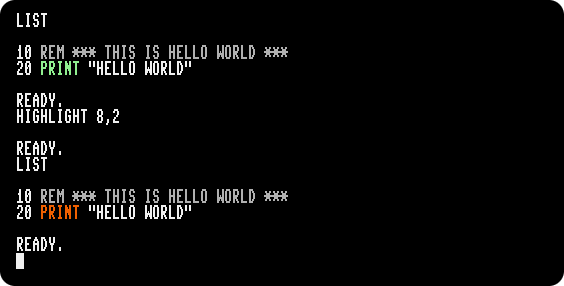
\includegraphics[width=0.8\linewidth]{images/highlight-example.png}\end{center}
\end{description}

% **
% IF
% **

\newpage
\subsection{IF}
\index{BASIC 65 Commands!IF}
\begin{description}[leftmargin=2cm,style=nextline]
\item [Token:] \$8B
\item [Format:] {\bf IF} expression {\bf THEN} true clause
		[{\bf ELSE} false clause]
\item [Usage:] Starts a conditional execution
               statement.

                {\bf expression} a logical or numeric expression.
                A numeric expression is evaluated as {\bf FALSE}
                if the value is zero and {\bf TRUE} for any non-zero
                value.

                {\bf true clause} one or more statements starting
                directly after {\bf THEN} on the same line.
                A line number after {\bf THEN} performs a
                {\bf GOTO} to that line instead.

                {\bf false clause} one or more statements starting
                directly after {\bf ELSE} on the same line.
                A linenumber after {\bf ELSE} performs a
                {\bf GOTO} to that line instead.

\item [Remarks:]
               The standard {\bf IF ... THEN ... ELSE} structure
               is restricted to a single line. But the {\bf true clause}
               or {\bf false clause} may be expanded to several lines
               using a compound statement surrounded with
               {\bf BEGIN} and {\bf BEND}.
\item [Example:]
                Using {\bf IF}
\begin{tcolorbox}[colback=black,coltext=white]
\verbatimfont{\codefont}
\begin{verbatim}
1 REM IF
10 RED$=CHR$(28) : BLACK$=CHR$(144) : WHITE$=CHR$(5)
20 INPUT "ENTER A NUMBER";V
30 IF V<0 THEN PRINT RED$; : ELSE PRINT BLACK$;
40 PRINT V : REM PRINT NEGATIVE NUMBERS IN RED
50 PRINT WHITE$
60 INPUT "END PROGRAM: (Y/N)"; A$
70 IF A$="Y" THEN END
80 IF A$="N" THEN 20 : ELSE 60
\end{verbatim}
\end{tcolorbox}
\end{description}

% *****
% INPUT
% *****

\newpage
\subsection{INPUT}
\index{BASIC 65 Commands!INPUT}
\begin{description}[leftmargin=2cm,style=nextline]
\item [Token:] \$85
\item [Format:] {\bf INPUT} [prompt <{\bf,} | {\bf;}>]
		variable [{\bf,} variable ...]
\item [Usage:] Prints an optional
               prompt string and question mark to the screen,
               flashes the cursor and waits for user input
               from the keyboard.

               {\bf prompt} optional string expression to be printed
               as the prompt.
               If the separator between {\bf prompt} and {\bf variable list}
               is a comma, the cursor is placed directly after
               the prompt. If the separator is a semicolon,
               a question mark and a space is added to the prompt instead.

               {\bf variable list} list of one or more
               variables that receive the input.

               The input will be processed after the user presses \specialkey{RETURN}.

\item [Remarks:] The user must take care to enter the correct
               type of input, so it matches the {\bf variable list} types.
               Also, the number of input items must match the number
               of variables. A surplus of input items will be ignored,
               too few input items trigger another request for input
               with the prompt ??.
               Typing non numeric characters for integer or real
               variables will produce a TYPE MISMATCH ERROR.
               Strings for string variables must be in double quotes (")
               if they contain spaces or commas.
               Many programs that need a safe input routine use
               {\bf LINE INPUT} and a custom parser, in order
               to avoid program errors by wrong user input.

\item [Example:] Using {\bf INPUT}:
\begin{tcolorbox}[colback=black,coltext=white]
\verbatimfont{\codefont}
\begin{verbatim}
 10 DIM N$(100),A%(100),S$(100):
 20 DO
 30 INPUT "NAME, AGE, GENDER";NA$,AG%,SE$
 40 IF NA$="" THEN 30
 50 IF NA$="END" THEN EXIT
 60 IF AG% < 18 OR AG% > 100 THEN PRINT "AGE?":GOTO 30
 70 IF SE$ <> "M" AND SE$ <> "F" THEN PRINT "GENDER?":GOTO 30
 80 REM CHECK OK: ENTER INTO ARRAY
 90 N$(N)=NA$:A%(N)=AG%:S$(N)=SE$:N=N+1
100 LOOP UNTIL N=100
110 PRINT "RECEIVED";N;" NAMES"
\end{verbatim}
\end{tcolorbox}
\end{description}

% *******
% INPUT\#
% *******

\newpage
\subsection{INPUT\#}
\index{BASIC 65 Commands!INPUT\#}
\begin{description}[leftmargin=2cm,style=nextline]
\item [Token:] \$84
\item [Format:] {\bf INPUT\#} channel{\bf,} variable [{\bf,} variable ...]
\item [Usage:] Reads a record
               from an input device, e.g. a disk file
               and assigns the data
               to the variables in the list.

               {\bf channel} number, which was given to a previous
               call to commands such as {\bf DOPEN}, or {\bf OPEN}.


               {\bf variable list} list of one or more
               variables, that receive the input.

               The input record must be terminated by a
               RETURN character and must be not longer than
               the input buffer (160 characters).

\item [Remarks:] The type and number of data in a record must
               match the variable list.
               Reading non numeric characters for integer or real
               variables will produce a FILE DATA ERROR.
               Strings for string variables have to be put in quotes
               if they contain spaces or commas. \\
               {\bf LINE INPUT\#} may be used to
               read a whole record into a single string variable.

               Sequential files, that can be read by {\bf INPUT\#}
               can be generated by programs with {\bf PRINT\#}
               or with the editor of the MEGA65.
               For example:

\begin{tcolorbox}[colback=black,coltext=white]
\verbatimfont{\codefont}
\begin{verbatim}
EDIT ON

10 "CHUCK PEDDLE",1937,"ENGINEER OF THE 6502"
20 "JACK TRAMIEL",1928,"FOUNDER OF CBM"
30 "BILL MENSCH",1945,"HARDWARE"

DSAVE "CBM-PEOPLE"
EDIT OFF
\end{verbatim}
\end{tcolorbox}

\item [Example:] Using {\bf INPUT\#}:
\begin{tcolorbox}[colback=black,coltext=white]
\verbatimfont{\codefont}
\begin{verbatim}
 10 DIM N$(100),B%(100),S$(100):
 20 DOPEN#2,"CBM-PEOPLE":REM OPEN SEQ FILE
 25 IF DS THEN PRINT DS$:STOP:REM OPEN ERROR
 30 FOR I=0 TO 100
 40 INPUT#2,N$(I),B%(I),S$(I)
 50 IF ST AND 64 THEN 80:REM END OF FILE
 60 IF DS THEN PRINT DS$:GOTO 80:REM DISK ERROR
 70 NEXT I
 80 DCLOSE#2
110 PRINT "READ";I;" RECORDS"
120 FOR J=0 TO I:PRINT N$(I):NEXT J

RUN
CHUCK PEDDLE
JACK TRAMIEL
BILL MENSCH

TYPE "CBM-PEOPLE"
"CHUCK PEDDLE",1937,"ENGINEER OF THE 6502"
"JACK TRAMIEL",1928,"FOUNDER OF CBM"
"BILL MENSCH",1945,"HARDWARE"

\end{verbatim}
\end{tcolorbox}
\end{description}

% *****
% INSTR
% *****

\newpage
\subsection{INSTR}
\index{BASIC 65 Commands!INSTR}
\begin{description}[leftmargin=2cm,style=nextline]
\item [Token:] \$D4
\item [Format:] {\bf INSTR(}haystack{\bf,} needle [{\bf,} start]{\bf)}
\item [Usage:] Locates the
               position of the string expression {\bf needle}
               in the string expression {\bf haystack}, and
               returns the index of the first occurrence,
               or zero if there is no match.

               The string expression {\bf haystack}
               is searched for the occurrence of the
               string expression
               {\bf needle}.

               An enhanced version of string search using pattern
               matching is used if the first character of
               the search string is a pound sign '£'.
               The pound sign is not part of the search but enables the use
               of the {\bf '.'} (dot) as a wildcard character, which matches any
               character. The second special pattern character is
               the {\bf '*'} (asterisk). The asterisk in the search string indicates
               that the preceding character may appear never, once or repeated
               in order to be considered as a match.

               The optional argument {\bf start} is an integer
               expression, which defines the starting position
               for the search in {\bf haystack}. If not present,
               it defaults to one.

\item [Remarks:] If either string is empty or there is no match
               the function returns zero.

\item [Examples:] Using {\bf INSTR}:
\begin{tcolorbox}[colback=black,coltext=white]
\verbatimfont{\codefont}
\begin{verbatim}
 I = INSTR("ABCDEF","CD")       : REM I = 3
 I = INSTR("ABCDEF","XY")       : REM I = 0
 I = INSTR("RAIIIN","\A*IN")    : REM I = 5
 I = INSTR("ABCDEF","\C.E")     : REM I = 3
 I = INSTR(A$+B$,C$)
\end{verbatim}
\end{tcolorbox}
\end{description}

%****
% INT
%****

\newpage
\subsection{INT}
\index{BASIC 65 Functions!INT}
\begin{description}[leftmargin=2cm,style=nextline]
\item [Token:] \$B5
\item [Format:] {\bf INT(}numeric expression{\bf)}
\item [Usage:] Returns the integer part of the argument.
               This function is {\bf NOT} limited to the typical
               16-bit integer range (-32768 to 32767), as
               it uses real arithmetic. The allowed range is
               therefore determined by the size of the real
               mantissa which is 32-bits wide (-2147483648 to 2147483647).

\item [Remarks:] It is not necessary to use the {\bf INT}
               function for assigning real values to integer
               variables, as this conversion will be done
               implicitly, but only for the 16-bit range.

\item [Examples:] Using {\bf INT}:
\begin{tcolorbox}[colback=black,coltext=white]
\verbatimfont{\codefont}
\begin{verbatim}
 X  = INT(1.9)       :REM X = 1
 X  = INT(-3.1)      :REM X = -3
 X  = INT(100000.5)  :REM X = 100000
 N% = INT(100000.5)  :REM ?ILLEGAL QUANTITY ERROR
\end{verbatim}
\end{tcolorbox}
\end{description}

%****
% JOY
%****

\newpage
\subsection{JOY}
\index{BASIC 65 Functions!JOY}
\begin{description}[leftmargin=2cm,style=nextline]
\item [Token:] \$CF
\item [Format:] {\bf JOY(}port{\bf)}
\item [Usage:] Returns the state of the
               joystick for the selected port (1 or 2).
               Bit 7 contains the state of the fire button.
               The stick can be moved in eight directions, which
               are numbered clockwise starting at the upper position.
\begin{center}
\ttfamily
{\setlength{\tabcolsep}{1mm}
\begin{tabular}{|r|c|c|c|}
\hline
&  left  & centre & right \\
\hline
up     &  8 &    1  & 2 \\
centre &  7 &    0  & 3 \\
down   &  6 &    5  & 4 \\
\hline
\end{tabular}
}
\end{center}

\item [Example:] Using {\bf JOY}:
\begin{tcolorbox}[colback=black,coltext=white]
\verbatimfont{\codefont}
\begin{verbatim}
 10 N = JOY(1)
 20 IF N AND 128 THEN PRINT "FIRE! ";
 30 REM                N   NE  E   SE  S   SW  W   NW
 40 ON N AND 15 GOSUB 100,200,300,400,500,600,700,800
 50 GOTO 10
100 PRINT "GO NORTH"    :RETURN
200 PRINT "GO NORTHEAST":RETURN
300 PRINT "GO EAST"     :RETURN
400 PRINT "GO SOUTHEAST":RETURN
500 PRINT "GO SOUTH"    :RETURN
600 PRINT "GO SOUTHWEST":RETURN
700 PRINT "GO WEST"     :RETURN
800 PRINT "GO NORTHWEST":RETURN
\end{verbatim}
\end{tcolorbox}
\end{description}

%****
% KEY
%****

\newpage
\subsection{KEY}
\index{BASIC 65 Commands!KEY}
\begin{description}[leftmargin=2cm,style=nextline]
\item [Token:] \$F9
\item [Format:] {\bf KEY} \\
		{\bf KEY} <{\bf ON} | {\bf OFF}> \\
		{\bf KEY} <{\bf LOAD} | {\bf SAVE}> filename \\
		{\bf KEY} number{\bf,} string
\item [Usage:] Reads the state of the function keys.
               The function keys can either send their key code
               when pressed, or a string assigned to the key.
               After power up or reset this feature is activated
               and the keys have their default assignments.

               {\bf KEY} list current assignments.

               {\bf KEY ON} switch on function key strings.
               The keys will send assigned strings if pressed.

               {\bf KEY OFF} switch off function key strings.
               The keys will send their character code if pressed.

               {\bf KEY LOAD} loads key definitions from file.

               {\bf KEY SAVE} saves key definitions to file.

               {\bf KEY number, string} assigns the string to
               the key with the given number.

               Default assignments:

\begin{tcolorbox}[colback=black,coltext=white]
\verbatimfont{\codefont}
\begin{verbatim}
KEY
KEY 1,CHR$(27)+"X"
KEY 2,CHR$(27)+"@"
KEY 3,"DIR"+CHR$(13)
KEY 4,"DIR "+CHR$(34)+"*=PRG"+CHR$(34)+CHR$(13)
KEY 5,"ŵ"
KEY 6,"KEY6"+CHR$(141)
KEY 7,"ŷ"
KEY 8,"MONITOR"+CHR$(13)
KEY 9,"Ű"
KEY 10,"KEY10"+CHR$(141)
KEY 11,"Ŷ"
KEY 12,"KEY12"+CHR$(141)
KEY 13,CHR$(27)+"O"
KEY 14,"Ŵ"+CHR$(27)+"O"
KEY 15,"HELP"+CHR$(13)
KEY 16,"RUN "+CHR$(34)+"*"+CHR$(34)+CHR$(13)
\end{verbatim}
\end{tcolorbox}

\item [Remarks:] The sum of the lengths of all assigned strings
                 must not exceed 240 characters.
                 Special characters such as RETURN or QUOTE are entered
                 using their codes with the CHR\$(code) function.
                 Refer to {\bf CHR\$} on page \pageref{chrcommand}
                 for more information.

\item [Examples:] Using {\bf KEY}:
\begin{tcolorbox}[colback=black,coltext=white]
\verbatimfont{\codefont}
\begin{verbatim}
 KEY ON                   :REM ENABLE  FUNCTION KEYS
 KEY OFF                  :REM DISABLE FUNCTION KEYS
 KEY                      :REM LIST ASSIGNMENTS
 KEY 2,"PRINT ~"+CHR$(14) :REM ASSIGN PRINT PI TO F2
 KEY SAVE "MY KEY SET"    :REM SAVE CURRENT DEFINITIONS TO FILE
 KEY LOAD "ELEVEN-SET"    :REM LOAD DEFINITIONS FROM FILE
\end{verbatim}
\end{tcolorbox}
\end{description}

% ******
% LEFT\$
% ******

\newpage
\subsection{LEFT\$}
\index{BASIC 65 Functions!LEFT\$}
\begin{description}[leftmargin=2cm,style=nextline]
\item [Token:] \$C8
\item [Format:] {\bf LEFT\$(}string{\bf,} n{\bf)}
\item [Usage:] Returns a string
               containing the first {\bf n} characters from the
               argument {\bf string}.
               If the length of {\bf string} is equal to or less than {\bf n},
               the resulting string will be identical to the argument string.

               {\bf string} a string expression.

               {\bf n} a numeric expression (0-255).

\item [Remarks:] Empty strings and zero lengths are legal values.

\item [Example:] Using {\bf LEFT\$}:
\begin{tcolorbox}[colback=black,coltext=white]
\verbatimfont{\codefont}
\begin{verbatim}
PRINT LEFT$("MEGA-65",4)
MEGA
\end{verbatim}
\end{tcolorbox}
\end{description}

% ***
% LEN
% ***

\newpage
\subsection{LEN}
\index{BASIC 65 Functions!LEN}
\begin{description}[leftmargin=2cm,style=nextline]
\item [Token:] \$C3
\item [Format:] {\bf LEN(}string{\bf)}
\item [Usage:] Returns the length of a string.

               {\bf string} a string expression.

\item [Remarks:] There is no terminating character, as opposed to
                 other programming languages such as C, which uses
                 the NULL character. The length of
                 the string is internally stored in an extra byte of
                 the string descriptor.

\item [Example:] Using {\bf LEN}:
\begin{tcolorbox}[colback=black,coltext=white]
\verbatimfont{\codefont}
\begin{verbatim}
PRINT LEN("MEGA-65"+CHR$(13))
 8
\end{verbatim}
\end{tcolorbox}
\end{description}

% ***
% LET
% ***

\newpage
\subsection{LET}
\index{BASIC 65 Commands!LET}
\begin{description}[leftmargin=2cm,style=nextline]
\item [Token:] \$88
\item [Format:] {\bf [LET] variable = expression}
\item [Usage:] Assigns values (or results of expressions) to variables.
\item [Remarks:] The {\bf LET} statement is obsolete and not required.
               Assignment to variables can be done without using
               {\bf LET}, but it has been left in BASIC 65 for backwards compatibility.

\item [Examples:] Using {\bf LET}:
\begin{tcolorbox}[colback=black,coltext=white]
\verbatimfont{\codefont}
\begin{verbatim}
LET A=5  :REM LONGER  AND SLOWER
A=5      :REM SHORTER AND FASTER
\end{verbatim}
\end{tcolorbox}
\end{description}

% ****
% LINE
% ****

\newpage
\subsection{LINE}
\index{BASIC 65 Commands!LINE}
\begin{description}[leftmargin=2cm,style=nextline]
\item [Token:] \$E5
\item [Format:] {\bf LINE xbeg, ybeg [,xnext1, ynext1 [\dots]] }
\item [Usage:] Draws a pixel at (xbeg/ybeg), if only one
               coordinate pair is given.

               If more than one pair is defined, a line is
               drawn on the current graphics screen from the
               coordinate (xbeg/ybeg) to the next coordinate
               pair(s).

               All currently defined modes and values of the graphics
               context are used.

\item [Example:] Using {\bf LINE}:
\begin{tcolorbox}[colback=black,coltext=white]
\verbatimfont{\codefont}
\begin{verbatim}
1 REM SCREEN EXAMPLE 1
10 SCREEN 320,200,2      :REM SCREEN #0 320 X 200 X 2
20 PEN 1                 :REM DRAWING PEN COLOR 1 (WHITE)
30 LINE 25,25,295,175    :REM DRAW LINE
40 GETKEY A$             :REM WAIT FOR KEYPRESS
50 SCREEN CLOSE          :REM CLOSE SCREEN AND RESTORE PALETTE
\end{verbatim}
\end{tcolorbox}
\begin{tcolorbox}[colback=black,coltext=white]
\begin{center}
\begin{tikzpicture}[thick]
\draw (2cm,2cm) -- (5.5cm,0cm);
\end{tikzpicture}
\end{center}
\end{tcolorbox}
\end{description}

% ************
% LINE INPUT\#
% ************

\newpage
\subsection{LINE INPUT\#}
\index{BASIC 65 Commands!LINE INPUT\#}
\begin{description}[leftmargin=2cm,style=nextline]
\item [Token:] \$E5 \$84
\item [Format:] {\bf LINE INPUT\# channel, variable list}
\item [Usage:] Reads one record per variable from an input device,
              (such as a disk drive)
               and assigns the read data to the variable.
               The records must be terminated by a {\bf RETURN}
               character, which will not be copied to the string variable.
               Therefore, an empty line consisting of only the {\bf RETURN} character
               will result in an empty string being assigned.

               {\bf channel} number, which was given to a previous
               call to commands such as {\bf DOPEN}, or {\bf OPEN}.

               {\bf variable list} list of one or more
               variables, that receive the input.

\item [Remarks:] Only string variables or string array elements
                 can be used in the variable list.
                 Unlike other INPUT commands, {LINE INPUT\#} does
                 not interpret or remove quote characters in the input.
                 They are accepted as data, as all other characters.

                 Records must not be longer than the input buffer, which is 160 characters.

\item [Example:] Using {\bf LINE INPUT\#}:
\begin{tcolorbox}[colback=black,coltext=white]
\verbatimfont{\codefont}
\begin{verbatim}
 10 DIM N$(100)
 20 DOPEN#2,"DATA"
 30 FOR I=0 TO 100
 40 LINE INPUT#2,N$(I)
 50 IF ST=64 THEN 80:REM END OF FILE
 60 IF DS THEN PRINT DS$:GOTO 80:REM DISK ERROR
 70 NEXT I
 80 DCLOSE#2
110 PRINT "READ";I;" RECORDS"
\end{verbatim}
\end{tcolorbox}
\end{description}

% ****
% LIST
% ****

\newpage
\subsection{LIST}
\index{BASIC 65 Commands!LIST}
\begin{description}[leftmargin=2cm,style=nextline]
\item [Token:] \$9B
\item [Format:] {\bf LIST [P] [line range]}

\item [Usage:] Used to list a range of lines from the BASIC program.

               {\bf line range} consists of the first and/or last
               line to list, or a single line number.
               If the first number is omitted, the
               first BASIC line is assumed.
               If the second number is omitted, the last BASIC line
               is assumed.

\item [Format:] {\bf LIST [P] filename [,U unit]}

\item [Usage:] Used to list a BASIC program directly from {\bf unit},
               which by default is 8.

\item [Remarks:]

                The optional parameter {\bf P} enables page mode.
                After listing 24 lines, the listing will stop and display
                the prompt {\bf [MORE]} at the bottom of the screen.
                Pressing {\bf Q} quits page mode, while any other key
                triggers the listing of the next page.

                {\bf LIST} output can be redirected
                to other devices via {\bf CMD}.

                The keys \megakey{F9} and \megakey{F11}, or
                \specialkey{Ctrl}  \megakey{P} and
                \specialkey{Ctrl}  \megakey{V}
                scroll a BASIC listing on screen up or down.

\item [Examples:] Using {\bf LIST}
\begin{tcolorbox}[colback=black,coltext=white]
\verbatimfont{\codefont}
\begin{verbatim}
LIST 100      :REM LIST LINE 100
LIST 240-350  :REM LIST ALL LINES FROM 240 TO 350
LIST 500-     :REM LIST FROM 500 TO END
LIST -70      :REM LIST FROM START TO 70
LIST "DEMO"   :REM LIST FILE "DEMO"
LIST P        :REM LIST PROGRAM IN PAGE MODE
LIST P "MURX" :REM LIST FILE "MURX" IN PAGE MODE
\end{verbatim}
\end{tcolorbox}
\end{description}

% ****
% LOAD
% ****

\newpage
\subsection{LOAD}
\index{BASIC 65 Commands!LOAD}
\begin{description}[leftmargin=2cm,style=nextline]
\item [Token:] \$93
\item [Format:] {\bf LOAD filename [,unit [,flag]]} \\
                {\bf / filename [,unit [,flag]]}
\item [Usage:]

   A common use of the shortcut symbol {\bf /} is to quickly load
   {\bf PRG} files. To do this:

    \begin{enumerate}
    \item Print a disk directory using either {\bf DIR}, or {\bf CATALOG}.
    \item Move the cursor to the desired line.
    \item type {\bf /} in the first column of the line, and press \specialkey{RETURN}.
    \end{enumerate}
   After pressing \specialkey{RETURN}, the listed file on the line with the leading {\bf /} will be loaded.
Characters before and after the file name double quotes (") will be ignored.
   This applies to {\bf PRG} files only.

   {\bf filename} is either a quoted string, e.g. {\bf "prog"}, or
   a string expression.

   The unit number is optional.
   If not present, the default disk device is assumed.

   If {\bf flag} has a non-zero value, the file is loaded to
   the address which is read from the first two bytes of the file.
   Otherwise, it is loaded to the start of BASIC memory and
   the load address in the file is ignored.

\item [Remarks:]
   {\bf LOAD} loads files of type {\bf PRG} into RAM bank 0,
   which is also used for BASIC program source.

   {\bf LOAD "*"} can be used to load the first {\bf PRG} from the
   given {\bf unit}.

   {\bf LOAD "\$"} can be be used to load
   the list of files from the given {\bf unit}. When using {\bf LOAD "\$"},
   {\bf LIST} can be used to print the listing to screen.

   {\bf LOAD} is implemented in BASIC 65 to keep it backwards
   compatible with BASIC V2.

   The shortcut symbol {\bf /} can only be used in direct mode.

   By default the C64 uses {\bf unit} 1, which is assigned to datasette
   tape recorders connected to the cassette port. However the MEGA65
   uses {\bf unit} 8 by default, which is assigned to the internal
   disk drive. This means you don't need to add \screentext{,8} to
   {\bf LOAD} commands that use it.

\item [Examples:] Using {\bf LOAD}
\begin{tcolorbox}[colback=black,coltext=white]
\verbatimfont{\codefont}
\begin{verbatim}
  LOAD "APOCALYPSE"   :REM LOAD A FILE CALLED APOCALYPSE TO BASIC MEMORY
  LOAD "MEGA TOOLS",9 :REM LOAD A FILE CALLED "MEGA TOOLS" FROM UNIT 9 TO BASIC MEMORY
  LOAD "*",8,1        :LOAD THE FIRST FILE ON UNIT 8 TO RAM AS SPECIFIED IN THE FILE
\end{verbatim}
\end{tcolorbox}
\end{description}

% *******
% LOADIFF
% *******

\newpage
\subsection{LOADIFF}
\index{BASIC 65 Commands!LOADIFF}
\begin{description}[leftmargin=2cm,style=nextline]
\item [Token:] \$FE \$43
\item [Format:] {\bf LOADIFF filename [,D drive] [,U unit]}
\item [Usage:]

   Loads an IFF file into graphics memory.
   The IFF (Interchange File Format) is supported by many different applications
   and operating systems. {\bf LOADIFF} assumes that files
   contain bitplane graphics which fit into the MEGA65 graphics memory.
   Supported resolutions are:
\begin{center}
{\ttfamily
\setlength{\tabcolsep}{1mm}
\begin{tabular}{|l|l|l|l|l|}
\hline
 Width             & Height & Bitplanes & Colours & Memory \\
\hline
320                     &  200    & max. 8     & max. 256 & max. 64 K \\
640                     &  200    & max. 8     & max. 256 & max. 128 K \\
320                     &  400    & max. 8     & max. 256 & max. 128 K \\
640                     &  400    & max. 4     & max.  16 & max. 128 K \\
\hline
\end{tabular}
}
\end{center}

   \filenamedefinition

   \drivedefinition

   \unitdefinition

\item [Remarks:]
   Tools are available to convert popular image formats to IFF. These tools
   are available on several operating systems, such as AMIGA OS, macOS, Linux, and Windows.
   For example, {\bf ImageMagick} is a free graphics package that includes a tool
   called {\bf convert}, which can be used to create IFF files in conjunction
   with the {\bf ppmtoilbm} tool from the {\bf Netbpm} package.

To use {\bf convert} and {\bf ppmtoilbm} for converting a JPG file to an IFF file on Linux:

\begin{verbatim}
convert <myImage.jpg> <myImage.ppm>
ppmtoilbm -aga <myImage.pbm> > <myImage.iff>
\end{verbatim}

\item [Example:] Using {\bf LOADIFF}
\begin{tcolorbox}[colback=black,coltext=white]
\verbatimfont{\codefont}
\begin{verbatim}
100 BANK128:SCNCLR
110 REM DISPLAY PICTURES IN 320 X 200 X 7 RESOLUTION
120 GRAPHIC CLR:SCREEN DEF 0,0,0,7:SCREEN OPEN 0:SCREEN SET 0,0
130 FORI=1TO7: READF$
140 LOADIFF(F$+".IFF"):SLEEP 4:NEXT
150 DATA ALIEN,BEAKER,JOKER,PICARD,PULP,TROOPER,RIPLEY
160 SCREEN CLOSE 0
170 PALETTE RESTORE
\end{verbatim}
\end{tcolorbox}
\end{description}

% ***
% LOG
% ***

\newpage
\subsection{LOG}
\index{BASIC 65 Functions!LOG}
\begin{description}[leftmargin=2cm,style=nextline]
\item [Token:] \$BC
\item [Format:] {\bf LOG(numeric expression)}
\item [Usage:] Computes
               the value of the natural logarithm of the argument.
               The natural logarithm uses
               Euler's number ({\bf 2.71828183}) as base,
               not 10 which is typically used
               in log functions on a pocket calculator.

\item [Remarks:] The log function with base 10 can be computed
                 by dividing the result by log(10).
\item [Example:] Using {\bf LOG}
\begin{tcolorbox}[colback=black,coltext=white]
\verbatimfont{\codefont}
\begin{verbatim}
PRINT LOG(1)
 0

PRINT LOG(0)
 ?ILLEGAL QUANTITY ERROR

PRINT LOG(4)
 1.38629436

PRINT LOG(100) / LOG(10)
 2
\end{verbatim}
\end{tcolorbox}
\end{description}

% *****
% LOG10
% *****

\newpage
\subsection{LOG10}
\index{BASIC 65 Functions!LOG10}
\begin{description}[leftmargin=2cm,style=nextline]
\item [Token:] \$CE \$08
\item [Format:] {\bf LOG10(numeric expression)}
\item [Usage:] Computes
               the value of the decimal logarithm of the argument.
               The decimal logarithm uses 10 as base.

\item [Example:] Using {\bf LOG10}
\begin{tcolorbox}[colback=black,coltext=white]
\verbatimfont{\codefont}
\begin{verbatim}
PRINT LOG10(1)
 0

PRINT LOG10(0)
 ?ILLEGAL QUANTITY ERROR

PRINT LOG10(5)
 0.69897

PRINT LOG10(100);LOG(10);LOG(0.1);LOG(0.01)
 2  1 -1 -2
\end{verbatim}
\end{tcolorbox}
\end{description}

% ****
% LOOP
% ****

\newpage
\subsection{LOOP}
\index{BASIC 65 Commands!LOOP}
\begin{description}[leftmargin=2cm,style=nextline]
\item [Token:] \$EC
\item [Format:] {\bf DO} ... {\bf LOOP} \\
                {\bf DO} [<{\bf UNTIL} | {\bf WHILE}> logical expression] \\
                . . . statements [{\bf EXIT}] \\
                {\bf LOOP} [<{\bf UNTIL} | {\bf WHILE}> logical expression]
\item [Usage:] {\bf DO} and {\bf LOOP} define
                the start of a BASIC loop.
                Using {\bf DO} and {\bf LOOP} alone without any
                modifiers creates an infinite loop, which can only be exited
                by the {\bf EXIT} statement. The loop can be
                controlled by adding {\bf UNTIL} or {\bf WHILE}
                after the {\bf DO} or {\bf LOOP}.


\item [Remarks:] {\bf DO} loops may be nested. An {\bf EXIT} statement
only exits the current loop.
\item [Examples:] Using {\bf DO} and {\bf LOOP}
\begin{tcolorbox}[colback=black,coltext=white]
\verbatimfont{\codefont}
\begin{verbatim}
10 PW$="":DO
20 GET A$:PW$=PW$+A$
30 LOOP UNTIL LEN(PW$)>7 OR A$=CHR$(13)

10 DO : REM WAIT FOR USER DECISION
20 GET A$
30 LOOP UNTIL A$="Y" OR A$="N" OR A$="y" OR A$="n"

10 DO WHILE ABS(EPS) > 0.001
20 GOSUB 2000 : REM ITERATION SUBROUTINE
30 LOOP

10 I%=0 : REM INTEGER LOOP 1-100
20 DO I%=I%+1
30 LOOP WHILE I% < 101
\end{verbatim}
\end{tcolorbox}
\end{description}

% ****
% LPEN
% ****

\newpage
\subsection{LPEN}
\index{BASIC 65 Functions!LPEN}
\begin{description}[leftmargin=2cm,style=nextline]
\item [Token:] \$CE \$04
\item [Format:] {\bf LPEN(coordinate)}
\item [Usage:] This function requires the use of a
               CRT monitor (or TV), and a light pen.
               It will not work with an LCD or LED screen.
               The light pen must be connected to port 1.

               {\bf LPEN(0)} returns the X position of the light pen,
               the range is 60-320.

               {\bf LPEN(1)} returns the Y position of the light pen,
               the range is 50-250.

\item [Remarks:] The X resolution is two pixels, therefore {\bf LPEN(0)} only
                 returns even numbers.
                 A bright background colour is needed to trigger
                 the light pen. The {\bf COLLISION} statement may
                 be used to enable an interrupt handler.

\item [Example:] Using {\bf LPEN}
\begin{tcolorbox}[colback=black,coltext=white]
\verbatimfont{\codefont}
\begin{verbatim}
 PRINT LPEN(0),LPEN(1)   :REM PRINT LIGHT PEN COORDINATES
\end{verbatim}
\end{tcolorbox}
\end{description}

% *****
% MERGE
% *****

\newpage
\subsection{MERGE}
\index{BASIC 65 Commands!MERGE}
\begin{description}[leftmargin=2cm,style=nextline]
\item [Token:] \$E6
\item [Format:] {\bf MERGE filename [,D drive] [,U unit] }
\item [Usage:] {\bf MERGE} loads a BASIC program file from disk
               and appends it to the program in memory.

   \filenamedefinition

   \drivedefinition

   \unitdefinition

\item [Remarks:]
   The load address, stored in the first two bytes
   of the file is ignored. The loaded program does not
   replace a program in memory (which is what {\bf DLOAD} does),
   but is appended to a program in memory.
   After loading the program is re-linked
   and ready to run or edit.

   It is the user's responsibility to ensure that there
   are no line number conflicts among the program in memory and
   the merged program. The first line number of the merged
   program must be greater than the last line number of the
   program in memory.

\item [Example:] Using {\bf MERGE}
\begin{tcolorbox}[colback=black,coltext=white]
\verbatimfont{\codefont}
\begin{verbatim}
  DLOAD "MAIN PROGRAM"
  MERGE "LIBRARY"
\end{verbatim}
\end{tcolorbox}
\end{description}

% *****
% MID\$
% *****

\newpage
\subsection{MID\$}
\index{BASIC 65 Functions!MID\$}
\begin{description}[leftmargin=2cm,style=nextline]
\item [Token:] \$CA
\item [Format:] {\bf MID\$(}string{\bf,} index{\bf,} n{\bf)} \\
                {\bf MID\$(}string{\bf,} index{\bf,} n{\bf) =} string expression
\item [Usage:]  {\bf MID\$} can be used either as a function
                which returns a string, or as a statement for
                inserting sub-strings into an existing string.

               {\bf string} a string expression.

               {\bf index} start index (0-255).

               {\bf n} length of sub-string (0-255).

\item [Remarks:] Empty strings and zero lengths are legal values.

\item [Example:] Using {\bf MID\$}:
\begin{tcolorbox}[colback=black,coltext=white]
\verbatimfont{\codefont}
\begin{verbatim}
10 A$ = "MEGA-65"
20 PRINT MID$(A$,3,4)
30 MID$(A$,5,1) = "+"
40 PRINT A$
RUN
GA-6
MEGA+65
\end{verbatim}
\end{tcolorbox}
\end{description}

% ***
% MOD
% ***

\newpage
\subsection{MOD}
\index{BASIC 65 Functions!MOD}
\begin{description}[leftmargin=2cm,style=nextline]
\item [Token:] \$NN
\item [Format:] {\bf MOD(dividend, divisor)}
\item [Usage:] The {\bf MOD} function returns the remainder of the
      division.
\item [Remarks:] In other programming languages such C, this function
      is implemented as an operator (\%). In BASIC 65 it is implemented as a function.

\item [Example:] Using {\bf MOD}:
\begin{tcolorbox}[colback=black,coltext=white]
\verbatimfont{\codefont}
\begin{verbatim}
FOR I = 0 TO 8: PRINT MOD(I,4);: NEXT I
 0  1  2  3  0  1  2  3  0
\end{verbatim}
\end{tcolorbox}
\end{description}

% *******
% MONITOR
% *******

\newpage
\subsection{MONITOR}
\index{BASIC 65 Commands!MONITOR}
\begin{description}[leftmargin=2cm,style=nextline]
\item [Token:] \$FA
\item [Format:] {\bf MONITOR}
\item [Usage:]  Calls the machine language
                monitor program, which is mainly used for
                debugging.

\item [Remarks:] Using the {\bf MONITOR} requires knowledge
                 of the CSG4510 / 6502 / 6510 CPU,
                 the assembly language they use, and their
                 architectures. More information on the
                 {\bf MONITOR} is available in
\ifdefined\printmanual
the {\bf MEGA65 Book}.
\else
\bookvref{cha:MLMonitor}.
\fi

                 To exit the monitor press {\bf X}.

                 Help text can be displayed with either {\bf ?} or {\bf H}.

\item [Example:] Using {\bf MONITOR}
\begin{tcolorbox}[colback=black,coltext=white]
\verbatimfont{\codefont}
\begin{verbatim}
 MONITOR
\end{verbatim}
\end{tcolorbox}
\item \begin{center}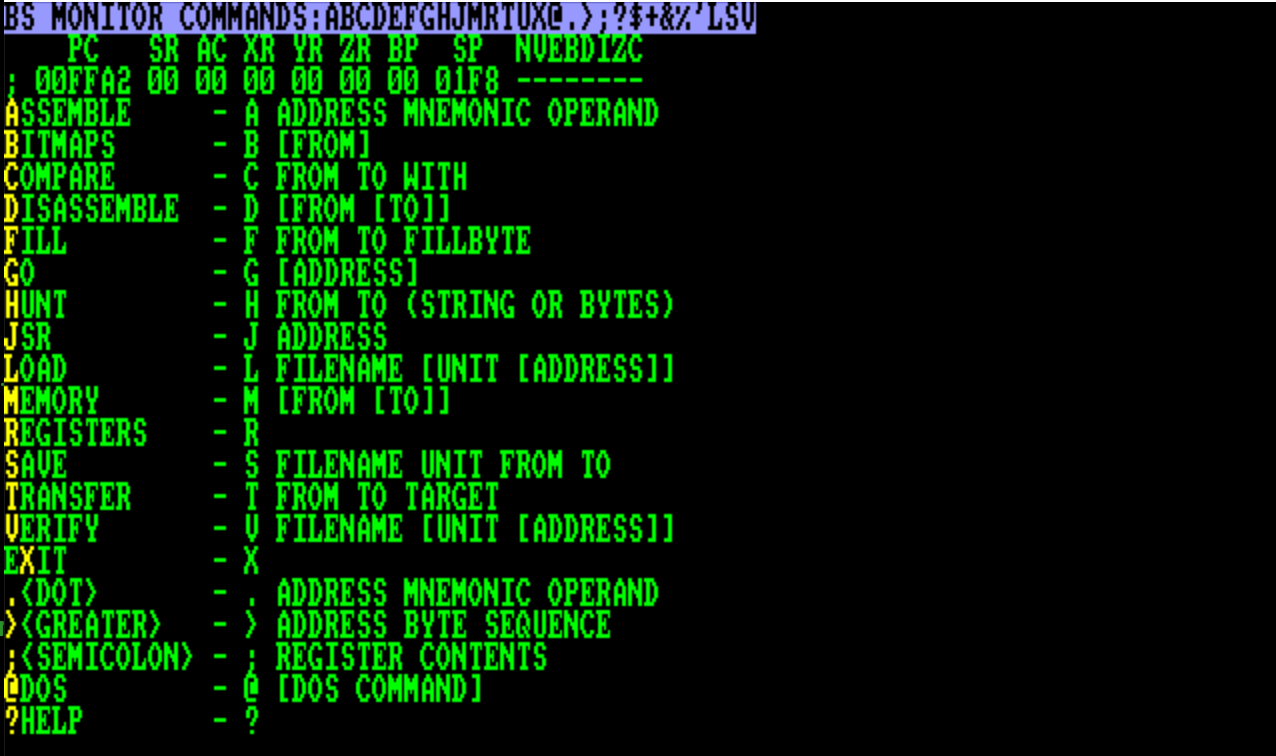
\includegraphics[width=0.8\linewidth]{images/monitor-h.png}\end{center}
\end{description}

% *****
% MOUSE
% *****

\newpage
\subsection{MOUSE}
\index{BASIC 65 Commands!MOUSE}
\begin{description}[leftmargin=2cm,style=nextline]
\item [Token:] \$FE \$3E
\item [Format:] {\bf MOUSE ON [\{,port, sprite, pos\}]} \\
                {\bf MOUSE OFF}
\item [Usage:]  Enables the mouse driver
                and connects the mouse at the specified port
                with the mouse pointer sprite.

                {\bf port} mouse port 1, 2 (default) or 3 (both).

                {\bf sprite} sprite number for mouse pointer (default 0).

                {\bf pos} initial mouse position (x,y).

                {\bf MOUSE OFF} disables the mouse
                driver and frees the associated sprite.

\item [Remarks:] The "hot spot" of the mouse pointer is the upper left
                pixel of the sprite.

\item [Examples:] Using {\bf MOUSE}:
\begin{tcolorbox}[colback=black,coltext=white]
\verbatimfont{\codefont}
\begin{verbatim}
 REM LOAD DATA INTO SPRITE #0 BEFORE USING IT
 MOUSE ON, 1       :REM ENABLE  MOUSE WITH SPRITE #0
 MOUSE OFF         :REM DISABLE MOUSE
\end{verbatim}
\end{tcolorbox}
\end{description}

% ******
% MOVSPR
% ******

\newpage
\subsection{MOVSPR}
\index{BASIC 65 Commands!MOVSPR}
\begin{description}[leftmargin=2cm,style=nextline]
\item [Token:] \$FE \$06
\item [Format:] {\bf MOVSPR number, position}
\item [Usage:]  Moves a sprite on screen. Each {\bf position} argument consists of two 16-bit values,
                which specify either an absolute coordinate, a relative coordinate,
                an angle, or a speed. The value type is determined by a prefix:

                \begin{itemize}
                    \item {\bf +value} relative coordinate: positive offset.
                    \item {\bf -value} relative coordinate: negative offset.
                    \item {\bf \#value} speed.
                \end{itemize}

                If no prefix is given, the absolute coordinate or angle is used.

                  Therefore, the position argument can be used to either:
                \begin{itemize}
                    \item set the sprite to an absolute position on screen.
                    \item specify a displacement relative from the current position.
                    \item trigger a relative movement from a specified position.
                    \item describe movement with an angle and speed starting from the current position.
                \end{itemize}

                {\bf MOVSPR number, position} is used to
                set the sprite immediately to the position or, in the case of
                an angle\#speed argument, describe its further movement.

\item [Format:] {\bf MOVSPR number, start-position TO end-position, speed}
\item [Usage:]  Places the sprite at the start position, defines the
                destination position, and the speed of movement.
                The sprite is placed at the start position, and will move
                in a straight line to the destination at the given speed.
                Coordinates must be absolute or relative.
                The movement is controlled by the BASIC interrupt handler and
                happens concurrently with the program execution.

                {\bf number} sprite number (0-7).

                {\bf position} x,y | xrel,y | x,yrel | xrel,yrel | angle\#speed.

                {\bf x} absolute screen coordinate pixel.

                {\bf y} absolute screen coordinate pixel.

                {\bf xrel} relative screen coordinate pixel.

                {\bf yrel} relative screen coordinate pixel.

                {\bf angle} compass direction for sprite movement [degrees].
                0 = up, 90 = right, 180 = down, 270 = left, 45 upper right, etc.

                {\bf speed} speed of movement, configured as a floating point number in the
                range of 0.0-127.0, in pixels per frame.
                PAL has 50 frames per second whereas NTSC has 60 frames per second.
                A speed value of 1.0 will move the sprite 50 pixels per second
                in PAL mode.


\item [Remarks:] The "hot spot" is the upper left pixel of the sprite.

\item [Example:] Using {\bf MOVSPR}:
\begin{tcolorbox}[colback=black,coltext=white]
\verbatimfont{\codefont}
\begin{verbatim}
100 CLR:SCNCLR:SPRITECLR
110 BLOAD "DEMOSPRITES1",B0,P1536
130 FORI=0TO7: C=I+1:SP=0.07*(I+1)
140 MOVSPRI, 160,120
145 MOVSPRI,45*I#SP
150 SPRITEI,1,C,,0,0
160 NEXT
170 SLEEP 3
180 FORI=0TO7:MOVSPR I,0#0:NEXT
\end{verbatim}
\end{tcolorbox}
\item \begin{center}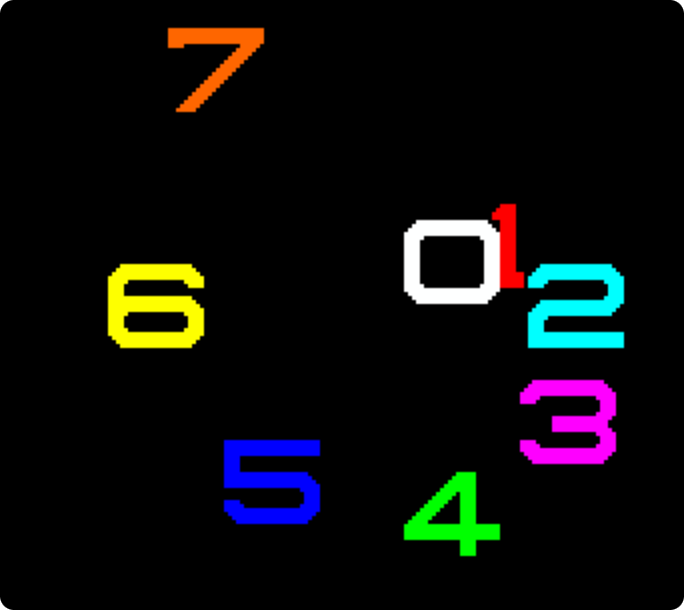
\includegraphics[width=0.8\linewidth]{images/sprites.png}\end{center}
\end{description}


% ***
% NEW
% ***

\newpage
\subsection{NEW}
\index{BASIC 65 Commands!NEW}
\begin{description}[leftmargin=2cm,style=nextline]
\item [Token:] \$A2
\item [Format:] {\bf NEW} \\
                {\bf NEW RESTORE}
\item [Usage:]  Resets all BASIC parameters to their default values.
                Since {\bf NEW} resets parameters and pointers,
                (but does not overwrite the address
                range of a BASIC program that was in memory),
                it is possible to recover the
                program. If there were no {\bf LOAD} operations,
                or editing performed after {\bf NEW}, the program
                can be restored with the {\bf NEW RESTORE}.
\item [Examples:] Using {\bf NEW}:
\begin{tcolorbox}[colback=black,coltext=white]
\verbatimfont{\codefont}
\begin{verbatim}
 NEW         :REM RESET BASIC
 NEW RESTORE :REM TRY TO RECOVER NEW'ED PROGRAM
\end{verbatim}
\end{tcolorbox}
\end{description}

% ****
% NEXT
% ****

\newpage
\subsection{NEXT}
\index{BASIC 65 Commands!NEXT}
\begin{description}[leftmargin=2cm,style=nextline]
\item [Token:] \$82
\item [Format:] {\bf FOR index=start TO end [STEP step] ... NEXT [index]}
\item [Usage:] Terminates the definition
               of a BASIC loop with an index variable.

               The {\bf index} variable may be incremented or decremented
               by a constant value {\bf step} on each iteration. The default
               is to increment the variable by 1.
               The index variable must be a real variable.

               {\bf start} value to initialise the index with.

               {\bf end} is checked at the end of an iteration,
               and determines whether another iteration will be performed,
               or if the loop will exit.

               {\bf step} defines the change applied to
               to the index variable at the end of every iteration.
               Positive step values increment it, while negative values
               decrement it. It defaults to 1.0 if not specified.

\item [Remarks:] The {\bf index} variable after {\bf NEXT} is
               optional. If it is omitted, the variable
               for the current loop is assumed.
               % i dont understand this part ^^ - impakt
               Several consecutive {\bf NEXT} statements may be
               combined by specifying the indexes in a comma
               separated list. The statements
               {\bf NEXT I:NEXT J:NEXT K} and
               {\bf NEXT I,J,K} are equivalent.

\item [Example:] Using {\bf NEXT}
\begin{tcolorbox}[colback=black,coltext=white]
\verbatimfont{\codefont}
\begin{verbatim}
10 FOR D=0 TO 360 STEP 30
20 R = D * ~ / 180
30 PRINT D;R;SIN(R);COS(R);TAN(R)
40 NEXT D

10 DIM M(20,20)
20 FOR I=0 TO 20
30 FOR J=I TO 20
40 M(I,J) = I + 100 * J
50 NEXT J,I
\end{verbatim}
\end{tcolorbox}
\end{description}

% ***
% NOT
% ***

\newpage
\subsection{NOT}
\index{BASIC 65 Operators!NOT}
\begin{description}[leftmargin=2cm,style=nextline]
\item [Token:] \$A8
\item [Format:] {\bf NOT} operand
\item [Usage:]  Performs a bit-wise
                logical NOT operation on a 16-bit value.
                Integer operands are used as they are, whereas
                real operands are converted to a signed 16-bit integer (losing precision).
                Logical operands are converted to a 16-bit integer,
                using \$FFFF (decimal -1) for TRUE,
                and \$0000 (decimal 0) for FALSE.

\begin{center}
{\ttfamily
\setlength{\tabcolsep}{1mm}
    \begin{tabular}{|l|l|l|}
    \hline
        expression & result  \\
    \hline
        NOT 0  &  1 \\
        NOT 1  &  0 \\
    \hline
\end{tabular}
}
\end{center}

\item [Remarks:] The result is of type integer.

\item [Examples:] Using {\bf NOT}

\begin{tcolorbox}[colback=black,coltext=white]
\verbatimfont{\codefont}
\begin{verbatim}
  PRINT NOT 3
  -4
  PRINT NOT 64
  -65
\end{verbatim}
\end{tcolorbox}

In most cases, {\bf NOT} is used in {\bf IF} statements.

\begin{tcolorbox}[colback=black,coltext=white]
\verbatimfont{\codefont}
\begin{verbatim}
   OK = C < 256 AND C >= 0
   IF (NOT OK) THEN PRINT "NOT A BYTE VALUE"
\end{verbatim}
\end{tcolorbox}
\end{description}

% ***
% OFF
% ***

\newpage
\subsection{OFF}
\index{BASIC 65 Commands!OFF}
\begin{description}[leftmargin=2cm,style=nextline]
\item [Token:] \$FE \$24
\item [Format:] {\bf keyword} {\bf OFF}
\item [Usage:]  {\bf OFF} is a secondary keyword used in
                combination with primary keywords, such as
                {\bf COLOR}, {\bf KEY}, and  {\bf MOUSE}.

\item [Remarks:] {\bf OFF} cannot be used on its own.

\item [Examples:] Using {\bf OFF}

\begin{tcolorbox}[colback=black,coltext=white]
\verbatimfont{\codefont}
\begin{verbatim}
  COLOR OFF :REM DISABLE SCREEN COLOUR
  KEY OFF   :REM DISABLE FUNCTION KEY STRINGS
  MOUSE OFF :REM DISABLE MOUSE DRIVER
\end{verbatim}
\end{tcolorbox}
\end{description}

% **
% ON
% **

\newpage
\subsection{ON}
\index{BASIC 65 Commands!ON}
\begin{description}[leftmargin=2cm,style=nextline]
\item [Token:] \$91
\item [Format:] {\bf ON expression GOSUB line list} \\
                {\bf ON expression GOTO line list}  \\
                {\bf keyword} {\bf ON}
\item [Usage:]  {\bf ON} calls
                either a computed {\bf GOSUB} or {\bf GOTO} statement.
                Depending on the result of the expression, the target
                for {\bf GOSUB} and {\bf GOTO} is chosen from
                the table of line addresses at the end of the statement.

                When used as a secondary keyword, {\bf ON} is used in
                combination with primary keywords, such as
                {\bf COLOR}, {\bf KEY}, and  {\bf MOUSE}.

                {\bf expression} is a positive numeric value.
                Real values are converted to integer (losing precision).
                Logical operands are converted to a 16-bit integer,
                using \$FFFF (decimal -1) for TRUE,
                and \$0000 (decimal 0) for FALSE.

                {\bf line list} is a comma separated list of valid
                line numbers.

\item [Remarks:] Negative values for {\bf expression} will stop
                 the program with an error message.
                 The {\bf line list} specifies the targets for values
                 of 1, 2, 3, etc. \\
                 An expression result of zero, or a result that is greater
                 than the number of target lines will not do anything, and the
                 program will continue execution with the next statement.

\newpage
\item [Example:] Using {\bf ON}
\begin{tcolorbox}[colback=black,coltext=white]
\verbatimfont{\codefont}
\begin{verbatim}
 10 COLOR ON :REM ENABLE SCREEN COLOUR
 20 KEY   ON :REM ENABLE FUNCTION KEY STRINGS
 30 MOUSE ON :REM ENABLE MOUSE DRIVER
 40 N = JOY(1):IF N AND 128 THEN PRINT "FIRE! ";
 60 REM                N   NE  E   SE  S   SW  W   NW
 70 ON N AND 15 GOSUB 100,200,300,400,500,600,700,800
 80 GOTO 40
100 PRINT "GO NORTH"    :RETURN
200 PRINT "GO NORTHEAST":RETURN
300 PRINT "GO EAST"     :RETURN
400 PRINT "GO SOUTHEAST":RETURN
500 PRINT "GO SOUTH"    :RETURN
600 PRINT "GO SOUTHWEST":RETURN
700 PRINT "GO WEST"     :RETURN
800 PRINT "GO NORTHWEST":RETURN
\end{verbatim}
\end{tcolorbox}
\end{description}

% ****
% OPEN
% ****

\newpage
\subsection{OPEN}
\index{BASIC 65 Commands!OPEN}
\begin{description}[leftmargin=2cm,style=nextline]
\item [Token:] \$9F
\item [Format:] {\bf OPEN channel, first address [,secondary address [,filename]]}
\item [Usage:]
   Opens an input/output channel for a device.

    {\bf channel} number, where:
    \begin{itemize}
        \item {\bf 1 <= channel <= 127} line terminator is CR.
        \item {\bf 128 <= channel <= 255} line terminator is CR LF.
    \end{itemize}

   {\bf first address} device number.
   For IEC devices the unit number is the primary address.
   Following primary address values are possible:

\begin{center}
{\setlength{\tabcolsep}{1mm}
\ttfamily
\begin{tabular}{|r|l|}
\hline
  unit  & device \\
\hline
  0 & Keyboard \\
  1 & System default \\
  2 & RS232 serial connection \\
  3 & Screen \\
  4-7 & IEC printer and plotter \\
  8-31 & IEC disk drives \\
\hline
\end{tabular}
}
\end{center}

   The {\bf secondary address} has some reserved values for
   IEC disk units, 0:load, 1:save, 15:command channel.
   The values 2-14 may be used for disk files.

   {\bf filename} is either a quoted string, e.g. {\bf "data"} or
   a string expression. The syntax is different to {\bf DOPEN\#},
   since the {\bf filename} for {\bf OPEN} includes all
   file attributes, for example "0:data,s,w".

\item [Remarks:]
   For IEC disk units the usage of {\bf DOPEN\#} is recommended.

   If the first character of the filename is an at sign '@', it
   is interpreted as a "save and replace" operation. It is not recommended
   to use this option on 1541 and 1571 drives, as they
   contain a "save and replace bug" in their DOS.

\item [Example:] Using {\bf OPEN}

\begin{tcolorbox}[colback=black,coltext=white]
\verbatimfont{\codefont}
\begin{verbatim}
   OPEN 4,4   :REM OPEN PRINTER
   CMD 4      :REM REDIRECT STANDARD OUTPUT TO 4
   LIST       :REM PRINT LISTING ON PRINTER DEVICE 4
   OPEN 3,8,3,"0:USER FILE,U"
   OPEN 2,9,2,"0:DATA,S,W"
\end{verbatim}
\end{tcolorbox}
\end{description}

% **
% OR
% **

\newpage
\subsection{OR}
\index{BASIC 65 Operators!OR}
\begin{description}[leftmargin=2cm,style=nextline]
\item [Token:] \$B0
\item [Format:] operand {\bf OR} operand
\item [Usage:]  Performs a bit-wise
                logical OR operation on two 16-bit values.
                Integer operands are used as they are.
                Real operands are converted to a signed 16-bit integer (losing precision).
                Logical operands are converted to a 16-bit integer
                using \$FFFF (decimal -1) for TRUE
                and \$0000 (decimal 0), for FALSE.

\begin{center}
{\ttfamily
\setlength{\tabcolsep}{1mm}
    \begin{tabular}{|l|l|l|}
        \hline
            expression & result  \\
        \hline
            0 OR 0  &  0 \\
            0 OR 1  &  1 \\
            1 OR 0  &  1 \\
            1 OR 1  &  1 \\
        \hline
    \end{tabular}
}
\end{center}


\item [Remarks:] The result is of type integer.
                 If the result is used in a logical context,
                 the value of 0 is regarded as FALSE, and
                 all other non-zero values are regarded as TRUE.
\item [Example:] Using {\bf OR}

\begin{tcolorbox}[colback=black,coltext=white]
\verbatimfont{\codefont}
\begin{verbatim}
  PRINT 1 OR 3
  3
  PRINT 128 OR 64
  192
\end{verbatim}
\end{tcolorbox}

In most cases, {\bf OR} is used in {\bf IF} statements.

\begin{tcolorbox}[colback=black,coltext=white]
\verbatimfont{\codefont}
\begin{verbatim}
   IF (C < 0 OR C > 255) THEN PRINT "NOT A BYTE VALUE"
\end{verbatim}
\end{tcolorbox}
\end{description}

% *****
% PAINT
% *****

\newpage
\subsection{PAINT}
\index{BASIC 65 Commands!PAINT}
\begin{description}[leftmargin=2cm,style=nextline]
\item [Token:] \$DF
\item [Format:] {\bf PAINT x, y, mode [,colour]}
\item [Usage:]  Performs a flood fill
                of an enclosed graphics area.

                {\bf x, y} is a coordinate pair, which must
                lie inside the area to be filled.

                {\bf mode} specifies the fill mode:
                \begin{itemize}
                    \item {\bf 0} use the {\bf colour} to fill the area.
                    \item {\bf 1} use the colour of pixel (x,y) to fill the area.
                \end{itemize}


\item [Example:] Using {\bf PAINT}

\begin{tcolorbox}[colback=black,coltext=white]
\verbatimfont{\codefont}
\begin{verbatim}
 10 GRAPHIC CLR          :REM INITIALISE
 20 SCREEN DEF 1,0,0,2   :REM 320 X 200
 30 SCREEN OPEN 1        :REM OPEN
 40 SCREEN SET 1,1       :REM MAKE SCREEN ACTIVE
 50 PALETTE 1,1,10,15,10 :REM COLOUR 1 TO LIGHT GREEN
 60 PEN 1                :REM SET DRAWING PEN (PEN 0) TO LIGHT GREEN (1)
 70 LINE 160,0,240,100   :REM 1ST. LINE
 80 LINE 240,100,80,100  :REM 2ND. LINE
 90 LINE 80,100,160,0    :REM 3RD. LINE
100 PAINT 160,10,0,1     :REM FILL TRIANGLE WITH COLOUR 1
110 GETKEY K$            :REM WAIT FOR KEY
120 SCREEN CLOSE 1       :REM END GRAPHICS
\end{verbatim}
\end{tcolorbox}
\end{description}

% *******
% PALETTE
% *******

\newpage
\subsection{PALETTE}
\index{BASIC 65 Commands!PALETTE}
\begin{description}[leftmargin=2cm,style=nextline]
\item [Token:] \$FE \$34
\item [Format:] {\bf PALETTE screen, colour, red, green, blue} \\
		{\bf PALETTE COLOR colour, red, green, blue} \\
                {\bf PALETTE RESTORE}
\item [Usage:]  {\bf PALETTE} can be used to change an
                entry of the system colour palette, or the palette
                of a screen. \\
                {\bf PALETTE RESTORE} resets the system palette to
                the default values.

                {\bf screen} screen number (0-3).

                {\bf COLOR} keyword for changing system palette.

                {\bf colour} index to palette (0-255).

                {\bf red} red intensity (0-15).

                {\bf green} green intensity (0-15).

                {\bf blue} blue intensity (0-15).

\item [Example:] Using {\bf PALETTE}

\begin{tcolorbox}[colback=black,coltext=white]
\verbatimfont{\codefont}
\begin{verbatim}
 10 REM CHANGE SYSTEM COLOUR INDEX
 20 REM --- INDEX  9 (BROWN) TO (DARK BLUE)
 30 PALETTE COLOR 9,0,0,7
\end{verbatim}
\end{tcolorbox}

\begin{tcolorbox}[colback=black,coltext=white]
\verbatimfont{\codefont}
\begin{verbatim}
 10 GRAPHIC CLR             :REM INITIALISE
 20 SCREEN DEF 1,0,0,2      :REM 320 X 200
 30 SCREEN OPEN 1           :REM OPEN
 40 SCREEN SET 1,1          :REM MAKE SCREEN ACTIVE
 50 PALETTE 1,0,  0, 0, 0   :REM 0 = BLACK
 60 PALETTE 1,1, 15, 0, 0   :REM 1 = RED
 70 PALETTE 1,2,  0, 0,15   :REM 2 = BLUE
 80 PALETTE 1,3,  0,15, 0   :REM 3 = GREEN
 90 PEN 2                   :REM SET DRAWING PEN (PEN 0) TO BLUE (2)
100 LINE 160,0,240,100      :REM 1ST. LINE
110 LINE 240,100,80,100     :REM 2ND. LINE
120 LINE 80,100,160,0       :REM 3RD. LINE
130 PAINT 160,10,0,2        :REM FILL TRIANGLE WITH BLUE (2)
140 GETKEY K$               :REM WAIT FOR KEY
150 SCREEN CLOSE 1          :REM END GRAPHICS
\end{verbatim}
\end{tcolorbox}
\end{description}

% ****
% PEEK
% ****

\newpage
\subsection{PEEK}
\index{BASIC 65 Functions!PEEK}
\begin{description}[leftmargin=2cm,style=nextline]
\item [Token:] \$C2
\item [Format:] {\bf PEEK(address)}
\item [Usage:]  Returns an unsigned 8-bit value (byte)
                from {\bf address}.

                If the address is in the range of \$0000 to \$FFFF (0-65535), the
                memory bank set by {\bf BANK} is used.

                Addresses greater than or equal to \$10000 (decimal 65536) are assumed to be flat memory
                addresses and used as such, ignoring the {\bf BANK} setting.

\item [Remarks:] Banks 0-127 give access to RAM or ROM banks.
                 Banks greater than 127 are used to access I/O, and the underlying SYSTEM hardware such as the
                 VIC, SID, FDC, etc.
\item [Example:] Using {\bf PEEK}

\begin{tcolorbox}[colback=black,coltext=white]
\verbatimfont{\codefont}
\begin{verbatim}
 10 BANK 128                :REM SELECT SYSTEM BANK
 20 L = PEEK($02F8)         :REM USR JUMP TARGET LOW
 30 H = PEEK($02F9)         :REM USR JUMP TARGET HIGH
 40 T = L + 256 * H         :REM 16-BIT JUMP ADDRESS
 50 PRINT "USR FUNCTION CALLS ADDRESS";T
\end{verbatim}
\end{tcolorbox}
\end{description}

% *****
% PEEKW
% *****

\newpage
\subsection{PEEKW}
\index{BASIC 65 Functions!PEEKW}
\begin{description}[leftmargin=2cm,style=nextline]
\item [Token:] \$C2 'W'
\item [Format:] {\bf PEEKW(address)}
\item [Usage:]  Returns an unsigned 16-bit value (word)
                read from {\bf address} (low byte) and {\bf address}+1 (high byte).

                If the address is in the range of \$0000 to \$FFFF (0-65535), the
                memory bank set by {\bf BANK} is used.

                Addresses greater than or equal to \$10000 (decimal 65536) are assumed to be flat memory
                addresses and used as such, ignoring the {\bf BANK} setting.


\item [Remarks:] Banks 0-127 give access to RAM or ROM banks.
                 Banks greater than 127 are used to access I/O, and the underlying SYSTEM hardware such as the
                 VIC, SID, FDC, etc.
\item [Example:] Using {\bf PEEKW}

\begin{tcolorbox}[colback=black,coltext=white]
\verbatimfont{\codefont}
\begin{verbatim}
 20 UA = PEEKW($02F8)   :REM USR JUMP TARGET
 50 PRINT "USR FUNCTION CALL ADDRESS";UA
\end{verbatim}
\end{tcolorbox}
\end{description}

% ***
% PEN
% ***

\newpage
\subsection{PEN}
\index{BASIC 65 Commands!PEN}
\begin{description}[leftmargin=2cm,style=nextline]
\item [Token:] \$FE \$33
\item [Format:] {\bf PEN [pen,] colour}
\item [Usage:]  Sets the colour of the graphic pen.

                {\bf pen} pen number (0-2):
                \begin{itemize}
                    \item {\bf 0} drawing pen (default, if only single parameter provided).
                    \item {\bf 1} off bits in jam2 mode.
                    \item {\bf 2} currently unused.
                \end{itemize}

                {\bf colour} palette index.

\item [Remarks:] The colour selected by {\bf PEN} will be used by all
                 graphic/drawing commands that follow it.
                 If you intend to set the drawing {\bf pen} 0 to a colour, you can
                 omit the first parameter, and only provide the {\bf colour} parameter.

\item [Example:] Using {\bf PEN}

\begin{tcolorbox}[colback=black,coltext=white]
\verbatimfont{\codefont}
\begin{verbatim}
 10 GRAPHIC CLR             :REM INITIALISE
 20 SCREEN DEF 1,0,0,2      :REM 320 X 200
 30 SCREEN OPEN 1           :REM OPEN
 40 SCREEN SET 1,1          :REM MAKE SCREEN ACTIVE
 50 PALETTE 1,0,  0, 0, 0   :REM 0 = BLACK
 60 PALETTE 1,1, 15, 0, 0   :REM 1 = RED
 70 PALETTE 1,2,  0, 0,15   :REM 2 = BLUE
 80 PALETTE 1,3,  0,15, 0   :REM 3 = GREEN
 90 PEN 1                   :REM SET DRAWING PEN (PEN 0) TO RED (1)
100 LINE 160,0,240,100      :REM DRAW RED LINE
110 PEN 2                   :REM SET DRAWING PEN (PEN 0) TO BLUE (2)
120 LINE 240,100,80,100     :REM DRAW BLUE LINE
130 PEN 3                   :REM SET DRAWING PEN (PEN 0) TO BLUE (3)
140 LINE 80,100,160,0       :REM DRAW GREEN LINE
150 GETKEY K$               :REM WAIT FOR KEY
160 SCREEN CLOSE 1          :REM END GRAPHICS
\end{verbatim}
\end{tcolorbox}
\end{description}



% *****
% PIXEL
% *****

\newpage
\subsection{PIXEL}
\index{BASIC 65 Functions!PIXEL}
\begin{description}[leftmargin=2cm,style=nextline]
\item [Token:] \$CE \$0C
\item [Format:] {\bf PIXEL(x,y)}
\item [Usage:]  Returns the colour of a pixel at the given position.

               {\bf x} absolute screen coordinate.

               {\bf y} absolute screen coordinate.
\end{description}

%TODO add example

% ****
% PLAY
% ****

\newpage
\subsection{PLAY}
\index{BASIC 65 Commands!PLAY}
\begin{description}[leftmargin=2cm,style=nextline]
\item [Token:] \$FE \$04
\item [Format:] {\bf PLAY [\{string1, string2, string3, string4, string5, string6\}]}
\item [Usage:] {\bf PLAY} without any arguments will cause all voices to be silenced,
               and all of BASIC's music-system variables to be reset (E.g. {\bf TEMPO}).

               {\bf PLAY} can be followed by up to six comma-separated string arguments,
               where each argument provides the sequence of notes and directives to be played on
               a specific voice on the two available SID chips, allowing for up to 6-channel polyphony.

               A musical note is a character (A, B, C, D, E, F, or G),
               which may be preceded by an optional modifier.

               Possible modifiers are:
\begin{center}
{\setlength{\tabcolsep}{1mm}
\ttfamily
\begin{tabular}{*{1}{|R{9mm}}|l|}
\hline
 char  & effect \\
\hline
 \# & sharp \\
 \$ & flat \\
  . & dotted \\
  H & half note \\
  I & eighth note \\
  Q & quarter note \\
  R & pause (rest) \\
  S & sixteenth note \\
  W & whole note \\
\hline
\end{tabular}
}
\end{center}

Embedded directives consist of a letter, followed by a digit:

\begin{center}
{\setlength{\tabcolsep}{1mm}
\ttfamily
\begin{tabular}{*{1}{|R{9mm}}|l|l|}
\hline
 char  & directive & argument range \\
\hline
  O & octave              & 0 - 6 \\
  T & instrument envelope & 0 - 9 \\
  U & volume              & 0 - 9 \\
  X & filter              & 0 - 1 \\
  M & modulation          & 0 - 9 \\
  P & portamento          & 0 - 9 \\
  L & loop                & N/A   \\
\hline
\end{tabular}
}
\end{center}

  The modulation directive will modulate your note by the magnitude you specify (1-9), or use 0 to turn this feature off.

    Similarly, the portamento directive will gently slide between consecutive notes at the speed you specify (1-9), or use 0 to turn this feature off. Note that the gate-off behaviour of notes is disabled while portamento is enabled, and to re-enable it, you must turn off portamento (P0).

    Add an {\bf L} directive (no argument needed) at the end of your string if you would like it to loop back to the
  beginning of your string upon completion.

  You have a lot of flexibility on which voice channels you choose to play your melodies on.
  For instance, you may decide to use only voice 1 and voice 4 for your melody, and spare
  the other channels for sound effects generated by {\bf SOUND}. Just skip the voices
  you're not using with {\bf PLAY}, by leaving those arguments empty:

\begin{tcolorbox}[colback=black,coltext=white]
\verbatimfont{\codefont}
\begin{verbatim}
  PLAY "O4EDCDEEERL",,,"O2CGEGCGEGL"
\end{verbatim}
\end{tcolorbox}

  You can even call {\bf PLAY} again to use the aforementioned unused channels, to play another melody
  alongside your first melody. For example, using voice2 and voice5 this time:

\begin{tcolorbox}[colback=black,coltext=white]
\verbatimfont{\codefont}
\begin{verbatim}
  PLAY ,"O5T2IGAGFEDCEGO6.QCL",,,"O3T2.QG.B O4ICO3GE.QCL"
\end{verbatim}
\end{tcolorbox}

  If you wish to assess whether a melody is playing on a voice channel, you can
  find out by checking the value returned from {\bf RPLAY(voice)}, where the voice parameter
  is a value from 1 to 6 indicating the voice channel. It will return either 1 (playing),
  or 0 (not playing).

  One caveat to be aware of is that BASIC strings have a maximum length of 255 bytes.
  If your melody needs to exceed this length, consider breaking up your melody into several
  strings, then use {\bf RPLAY(voice)} to assess when your first string has finished and then
  play the next string.

  Instrument envelope slots may be modified by using the {\bf ENVELOPE}
  statement. The default settings for the envelopes are on
page \pageref{envelopetable}.

\item [Remarks:] The {\bf PLAY} statement makes use of an interrupt
                 driven routine that starts parsing the string
                 and playing the melody. Program execution continues
                 with the next statement, and will not block until
                 the melody has finished.


\item [Example:] Using {\bf PLAY}
\begin{tcolorbox}[colback=black,coltext=white]
\verbatimfont{\codefont}
\begin{verbatim}
 5 REM *** SIMPLE LOOPING EXAMPLE ***
10 ENVELOPE 9,10,5,10,5,0,300
20 VOL 8
30 TEMPO 30
40 PLAY "O5T9HCIDCDEHCG IGAGFEFDEWCL", "O2T0QCGEGCGEG DBGB CGEGL"
\end{verbatim}
\end{tcolorbox}

\begin{tcolorbox}[colback=black,coltext=white]
\verbatimfont{\codefont}
\begin{verbatim}
 5 REM *** MODULATION + PORTAMENTO EXAMPLE ***
10 TEMPO 20
20 M$ = "M5 T2O5P0QD P5FP0RP5QG .AI#AQA HGQE.C IDQE HFQD .DI#CQD HEQ#CQO4HA"
30 M$ = M$ + "O5QDHFQG.AI#AQA HGQE.C IDQEFED#CO4BO5#C DO4AFD P0R L"
40 B$ = "T0QRO2H.D.F.CO1.A.#A.G.A QAIO2AGFE H.D.F.CO1.A.#A.AO2 .D DL"
50 PLAY M$,B$
\end{verbatim}
\end{tcolorbox}
\end{description}

% *******
% POINTER
% *******

\newpage
\subsection{POINTER}
\index{BASIC 65 Functions!POINTER}
\begin{description}[leftmargin=2cm,style=nextline]
\item [Token:] \$CE \$0A
\item [Format:] {\bf POINTER(variable)}
\item [Usage:]  Returns the current address of a variable
                or an array element as a 32-bit pointer.
                For string variables, it is the address of
                the string descriptor, not the string itself.
                The string descriptor consists of three bytes
                (length, string address low, string address high).

\item [Remarks:] The address values of arrays and their elements
                 are constant while the program is executing. \\
                 However, the addresses of strings (not their descriptors)
                 may change at any time due to
                 "garbage collection".

\item [Example:] Using {\bf POINTER}

\begin{tcolorbox}[colback=black,coltext=white]
\verbatimfont{\codefont}
\begin{verbatim}
10 BANK 0                  :REM SCALARS ARE IN BANK 0
20 H$="HELLO"              :REM ASSIGN STRING TO H$
30 P=POINTER(H$)           :REM GET DESCRIPTOR ADDRESS
40 PRINT "DESCRIPTOR AT: $";HEX$(P)
50 L=PEEK(P):SP=PEEKW(P+1) :REM LENGTH & STRING POINTER
60 PRINT "LENGTH = ";L     :REM PRINT LENGTH
70 BANK 1                  :REM STRINGS ARE IN BANK 1
80 FOR I%=0 TOL-1:PRINT PEEK(SP+I%);:NEXT:PRINT
90 FOR I%=0 TOL-1:PRINT CHR$(PEEK(SP+I%));:NEXT:PRINT

RUN
DESCRIPTOR AT: $F743
LENGTH =  5
 72  69  76  76  79
HELLO
\end{verbatim}
\end{tcolorbox}
\end{description}

% ****
% POKE
% ****

\newpage
\subsection{POKE}
\index{BASIC 65 Functions!POKE}
\begin{description}[leftmargin=2cm,style=nextline]
\item [Token:] \$97
\item [Format:] {\bf POKE address, byte [,byte ...] }
\item [Usage:]  Writes one or more bytes into memory
                or memory mapped I/O, starting at
                {\bf address}.

                If the address is in the range of \$0000 to \$FFFF (0-65535), the
                memory bank set by {\bf BANK} is used.

                Addresses greater than or equal to \$10000 (decimal 65536) are assumed to be flat memory
                addresses and used as such, ignoring the {\bf BANK} setting.

                {\bf byte} a value in the range of 0-255.

\item [Remarks:] The address is incremented for each data byte,
                 so a memory range can be written to with a single {\bf POKE}.

                 Banks greater than 127 are used to access I/O, and the underlying SYSTEM hardware such as the
                 VIC, SID, FDC, etc.


\item [Example:] Using {\bf POKE}

\begin{tcolorbox}[colback=black,coltext=white]
\verbatimfont{\codefont}
\begin{verbatim}
 10 BANK 128        :REM SELECT SYSTEM BANK
 20 POKE $02F8,0,24 :REM SET USR VECTOR TO $1800
\end{verbatim}
\end{tcolorbox}
\end{description}

% *****
% POKEW
% *****

\newpage
\subsection{POKEW}
\index{BASIC 65 Functions!POKEW}
\begin{description}[leftmargin=2cm,style=nextline]
\item [Token:] \$97 'W'
\item [Format:] {\bf POKEW address, word [,word ...] }
\item [Usage:]  Writes one or more words into memory
                or memory mapped I/O, starting at
                {\bf address}.

                If the address is in the range of \$0000 to \$FFFF (0-65535), the
                memory bank set by {\bf BANK} is used.

                Addresses greater than or equal to \$10000 (decimal 65536) are assumed to be flat memory
                addresses and used as such, ignoring the {\bf BANK} setting.

                {\bf word} a value from 0-65535.
                The first word is stored at address (low byte)
                and address+1 (high byte). The second word is stored at
                address+2 (low byte) and address+3 (high byte), etc.

\item [Remarks:] The address is increased by two for each data word,
                 so a memory range can be written to with a single {\bf POKEW}.

                Banks greater than 127 are used to access I/O, and the underlying SYSTEM hardware such as the
                VIC, SID, FDC, etc.
\item [Example:] Using {\bf POKEW}

\begin{tcolorbox}[colback=black,coltext=white]
\verbatimfont{\codefont}
\begin{verbatim}
 10 BANK 128                :REM SELECT SYSTEM BANK
 20 POKEW $02F8,$1800       :REM SET USR VECTOR TO $1800
\end{verbatim}
\end{tcolorbox}
\end{description}

% *******
% POLYGON
% *******

\newpage
\subsection{POLYGON}
\index{BASIC 65 Commands!POLYGON}

\begin{description}[leftmargin=2cm,style=nextline]
\item [Token:] \$FE \$2F
\item [Format:] {\bf POLYGON x, y, xrad, yrad, sides
                [\{,drawsides, subtend, angle, solid\}]}

\item [Usage:] Draws a regular {\bf n}-sided polygon.
               The polygon is drawn using the current drawing context
               set with {\bf SCREEN}, {\bf PALETTE}, and {\bf PEN}.

               {\bf x,y} centre coordinates.

               {\bf xrad,yrad} radius in x- and y-direction.

               {\bf sides} number of polygon sides.

               {\bf drawsides} sides to draw.

               {\bf subtend} draw line from centre to start (1).

               {\bf angle} start angle.

               {\bf solid} fill (1) or outline (0).

\item [Remarks:] A regular polygon is both isogonal and isotoxal,
                 meaning all sides and angles are alike.

\item [Example:] Using {\bf POLYGON}
\begin{tcolorbox}[colback=black,coltext=white]
\verbatimfont{\codefont}
\begin{verbatim}
100 SCREEN 320,200,1         :REM OPEN 320 x 200 SCREEN
110 POLYGON 160,100,40,40,6  :REM DRAW HONEYCOMB
120 GETKEY A$                :REM WAIT FOR KEY
130 SCREEN CLOSE             :REM CLOSE GRAPHICS SCREEN
\end{verbatim}
\end{tcolorbox}
Results in:
\begin{tcolorbox}[colback=black,coltext=white]
\begin{center}

\begin{tikzpicture}[thick]
\draw (4cm,2cm) -- (3cm,3mm) -- (1cm,3mm) -- (0cm,2cm) -- (1cm,37mm) -- (3cm,37mm) -- (4cm,2cm);
\end{tikzpicture}
\end{center}
\end{tcolorbox}
\end{description}

% ***
% POS
% ***

\newpage
\subsection{POS}
\index{BASIC 65 Functions!POS}
\begin{description}[leftmargin=2cm,style=nextline]
\item [Token:] \$B9
\item [Format:] {\bf POS(dummy)}
\item [Usage:]  Returns the cursor column relative to the
                currently used window.

                {\bf dummy} a numeric value, which is ignored.

\item [Remarks:] {\bf POS} gives the column position for the screen
                 cursor. It will not work for redirected output.

\item [Example:] Using {\bf POS}

\begin{tcolorbox}[colback=black,coltext=white]
\verbatimfont{\codefont}
\begin{verbatim}
 10 IF POS(0) > 72 THEN PRINT :REM INSERT RETURN
\end{verbatim}
\end{tcolorbox}
\end{description}

% ***
% POT
% ***

\newpage
\subsection{POT}
\index{BASIC 65 Functions!POT}
\begin{description}[leftmargin=2cm,style=nextline]
\item [Token:] \$CE \$02
\item [Format:] {\bf POT(paddle)}
\item [Usage:]  Returns the position of a paddle.

                {\bf paddle} paddle number (1-4).

                The low byte of the return value is the
                paddle value, with 0 at the clockwise limit and 255 at the
                anticlockwise limit.

                A value greater than 255 indicates that the fire button
                is also being pressed.

\item [Remarks:] Analogue paddles are noisy and inexact.
                 The range may be less than 0-255 and there
                 could be some jitter in the values returned from {\bf POT}.


\item [Example:] Using {\bf POT}

\begin{tcolorbox}[colback=black,coltext=white]
\verbatimfont{\codefont}
\begin{verbatim}
 10 X = POT(1)       : REM READ PADDLE #1
 20 B = X > 255      : REM TRUE (-1) IF FIRE BUTTON IS PRESSED
 30 V = X AND 255    : PADDLE #1 VALUE
\end{verbatim}
\end{tcolorbox}
\end{description}

% *****
% PRINT
% *****

\newpage
\subsection{PRINT}
\index{BASIC 65 Commands!PRINT}
\begin{description}[leftmargin=2cm,style=nextline]
\item [Token:] \$99
\item [Format:] {\bf PRINT arguments}
\item [Usage:]  Evaluates the argument list, and prints the values
                formatted to the current screen window.
                Standard formatting is used, depending on the
                argument type. For user controlled formatting,
                see {\bf PRINT USING}.

                The following argument types are evaluated:
                \begin{itemize}
                    \item {\bf numeric} the printout starts with a space
                    for positive and zero values, or a minus sign for
                    negative values. Integer values are printed with
                    the necessary number of digits. Real values are
                    printed in either fixed point form (typically
                    9 digits), or scientific form if the value is
                    outside the range of 0.01 to 999999999.

                    \item {\bf string} the string may consist of printable
                    characters and control codes. Printable characters
                    are printed at the cursor position, while control
                    codes are executed.

                    \item {\bf ","} a comma acts as a tabulator.

                    \item {\bf ";"} a semicolon acts as a separator between
                    arguments of the list. Other than the comma character,
                    it does not insert any additional characters.
                    A semicolon at the end of the argument list suppresses
                    the automatic return (carriage return) character.
                \end{itemize}
\item [Remarks:] The {\bf SPC} and {\bf TAB} functions
                 may be used in the argument list
                 for positioning.
                 {\bf CMD} can be used for redirection.

\item [Example:] Using {\bf PRINT}

\begin{tcolorbox}[colback=black,coltext=white]
\verbatimfont{\codefont}
\begin{verbatim}
 10 FOR I=1 TO 10    : REM START LOOP
 20 PRINT I,I*I,SQR(I)
 30 NEXT
\end{verbatim}
\end{tcolorbox}
\end{description}

% ******
% PRINT#
% ******

\newpage
\subsection{PRINT\#}
\index{BASIC 65 Commands!PRINT\#}
\begin{description}[leftmargin=2cm,style=nextline]
\item [Token:] \$98
\item [Format:] {\bf PRINT\# channel, arguments}
\item [Usage:]  Evaluates the argument list, and prints the formatted
                values to the device assigned to {\bf channel}.
                Standard formatting is used, depending on the
                argument type. For user controlled formatting,
                see {\bf PRINT\# USING}.

                {\bf channel} number, which was given to a previous
                call to commands such as {\bf APPEND}, {\bf DOPEN}, or {\bf OPEN}.

                The following argument types are evaluated:
                \begin{itemize}
                    \item {\bf numeric} the printout starts with a space
                    for positive and zero values, or a minus sign for
                    negative values. Integer values are printed with
                    the necessary number of digits. Real values are
                    printed in either fixed point form (typically
                    9 digits), or scientific form if the value is
                    outside the range of 0.01 to 999999999.

                    \item {\bf string} may consist of printable
                    characters and control codes. Printable characters
                    are printed at the cursor position, while control
                    codes are executed.

                    \item {\bf ","} a comma acts as a tabulator.

                    \item {\bf ";"} a semicolon acts as a separator between
                    arguments of the list. Other than the comma character,
                    it does not insert any additional characters.
                    A semicolon at the end of the argument list suppresses
                    the automatic return (carriage return) character.
                \end{itemize}

\item [Remarks:] The {\bf SPC} and {\bf TAB} functions
                 are not suitable for devices other than the screen.

\item [Example:] Using {\bf PRINT\#} to write a file to drive 8:

\begin{tcolorbox}[colback=black,coltext=white]
\verbatimfont{\codefont}
\begin{verbatim}
 10 DOPEN#2,"TABLE",W,U8
 20 FOR I=1 TO 10    : REM START LOOP
 30 PRINT#2,I,I*I,SQR(I)
 40 NEXT
 50 DCLOSE#2
\end{verbatim}
\end{tcolorbox}

    You can confirm that the file {\bf 'TABLE'} has been written by typing
    \screentext{DIR "TA*"}, and then view the contents of the file
    by typing \screentext{TYPE "TABLE"}.
\end{description}

% ***********
% PRINT USING
% ***********

\newpage
\subsection{PRINT USING}
\index{BASIC 65 Commands!PRINT USING}
\begin{description}[leftmargin=2cm,style=nextline]
\item [Token:] \$98 \$FB or \$99 \$FB
\item [Format:] {\bf PRINT [\# channel,] USING format;argument}
\item [Usage:]  Parses the {\bf format} string and evaluates the argument.
                The argument can be either a string or a numeric value.
                The format of the resulting output is directed
                by the {\bf format} string.

                {\bf channel} number, which was given to a previous
                call to commands such as {\bf APPEND}, {\bf DOPEN}, or {\bf OPEN}.
                If no channel is specified, the output goes to the screen.

                {\bf format} string variable or a string constant
                which defines the rules for formatting.
                When using a number as the {\bf argument}, formatting can be done in either
                CBM style, providing a pattern such as {\ttfamily \#\#\#.\#\#}
                or in C style using a <width.precision> specifier, such as {\ttfamily \%3D \%7.2F \%4X }.

                {\bf argument} the number to be formatted. If the argument does not fit into the format
                e.g. trying to print a 4 digit variable into {\ttfamily \#\#\#}
                a series of asterisks will replace the format character.

                {\bf argument} may consist of printable
                characters and control codes. Printable characters
                are printed to the cursor position, while control
                codes are executed.
                The number of {\ttfamily \#} characters sets the width of the output.
                If the first character of the format string
                is an equals '=' sign, the argument string is centered.
                If the first character of the format string
                is a greater than '>' sign, the argument string is right justified.

\item [Remarks:] The format string is applied for one argument only,
                 but it is possible to append more
                 {\bf USING format;argument} sequences.


\newpage
\item [Examples:] Using {\bf PRINT\# USING}

\begin{tcolorbox}[colback=black,coltext=white]
\verbatimfont{\codefont}
\begin{verbatim}
PRINT USING "##.##";~, USING " [%6.4F] ";SQR(2)
 3.14 [1.4142]

PRINT USING " < # # # > ";12*31
 < 3 7 2 >

PRINT USING "###"; "ABCDE"
ABC

PRINT USING ">###"; "ABCDE"
CDE

PRINT USING "ADDRESS:$%4X";65000
ADDRESS:$FDE8

A$="###,###,###.#":PRINT USING A$;1E8/3
 33,333,333.3
\end{verbatim}
\end{tcolorbox}
\end{description}

% *****
% PUDEF
% *****

%\newpage
%\subsection{PUDEF}
%\index{PUDEF}
%\index{BASIC 65 Commands!PUDEF}
%\begin{description}[leftmargin=2cm,style=nextline]
%\item [Token:] \$DD
%\item [Format:] {\bf PUDEF string}
%\item [Usage:]  Redefines up to four special characters, that are
%                used in the {\bf PRINT USING} routine.
%
%                {\bf string} = definition string (max. 4 characters).
%
%{\ttfamily
%                1st.: fill character \\
%                2nd.: comma separator \\
%                3rd.: decimal point \\
%                4th.: currency symbol
%
%                The system default is " ,.\$"
%}
%
%                The new definition string overrides the system
%                default and is often used for localisation.
%                A string " .," would change the punctuation to
%                German style.
%
%                It is not necessary to redefine all four characters.
%                Any length between 1 and 4 is allowed.
%
%\item [Remarks:] {\bf PUDEF} changes the output of {\bf PRINT USING}
%                 only. {\bf PRINT} and {\bf PRINT\#} are not affected.
%                 The control characters of the format string
%                 cannot be changed.
%
%\item [Example:] Using {\bf PUDEF}
%
%\begin{tcolorbox}[colback=black,coltext=white]
%\verbatimfont{\codefont}
%\begin{verbatim}
% 10 X = 123456.78
% 20 PUDEF " .,"
% 30 PRINT USING "###,###.#"; X : REM 123.456,8
%\end{verbatim}
%\end{tcolorbox}
%\end{description}

% ******
% RCOLOR
% ******

\newpage
\subsection{RCOLOR}
\index{BASIC 65 Functions!RCOLOR}
\begin{description}[leftmargin=2cm,style=nextline]
\item [Token:] \$CD
\item [Format:] {\bf RCOLOR(colour source)}
\item [Usage:]  Returns the current colour index for the
                selected colour source.

                Colour sources are:
                \begin{itemize}
                    \item {\bf 0} background colour (VIC \$D021).
                    \item {\bf 1} text colour (\$F1).
                    \item {\bf 2} highlight colour (\$2D8).
                    \item {\bf 3} border colour (VIC \$D020).
                \end{itemize}

\item [Example:] Using {\bf RCOLOR}

\begin{tcolorbox}[colback=black,coltext=white]
\verbatimfont{\codefont}
\begin{verbatim}
 10 C = RCOLOR(3)  : REM C = colour index of border colour
\end{verbatim}
\end{tcolorbox}
\end{description}

% *******
% RCURSOR
% *******

\newpage
\subsection{RCURSOR}
\index{BASIC 65 Commands!RCURSOR}
\begin{description}[leftmargin=2cm,style=nextline]
\item [Token:] \$FE \$42
\item [Format:] {\bf RCURSOR \{colvar, rowvar\}}
\item [Usage:]  Returns the current cursor column and row.

\item [Remarks:] The row and column values start at zero, where
                 the left-most column is zero, and the top row is zero.

\item [Example:] Using {\bf RCURSOR}

\begin{tcolorbox}[colback=black,coltext=white]
\verbatimfont{\codefont}
\begin{verbatim}
100 CURSOR ON,20,10
110 PRINT "[HERE]";
120 RCURSOR X,Y
130 PRINT " COL:";X;" ROW:";Y

RUN

                    [HERE] COL: 26  ROW: 10
\end{verbatim}
\end{tcolorbox}
\end{description}

% ****
% READ
% ****

\newpage
\subsection{READ}
\index{BASIC 65 Commands!READ}
\begin{description}[leftmargin=2cm,style=nextline]
\item [Token:] \$87
\item [Format:] {\bf READ variable list}
\item [Usage:]  Reads values from program source into variables.

               {\bf variable list} Any legal variables.

               All types of constants (integer, real, and
               strings) can be read, but not expressions.
               Items are separated by commas.
               Strings containing commas, colons or spaces must be put
               in quotes.

               {\bf RUN} initialises the data pointer
               to the first item of the first {\bf DATA} statement
               and advances it for every read item. It is the
               programmer's responsibility that the type of
               the constant and the variable in the {\bf READ}
               statement match. Empty items with no constant
               between commas are allowed and will be interpreted as
               zero for numeric variables and an empty string for
               string variables.

               {\bf RESTORE} may be used to set the
               data pointer to a specific line for subsequent
               readings.

\item [Remarks:] It is good programming practice to put large amounts of
                 {\bf DATA} statements at the end of the program,
                 so they don't slow down the search for line numbers
                 after {\bf GOTO}, and other statements with line number targets.

\item [Example:] Using {\bf READ}
\begin{tcolorbox}[colback=black,coltext=white]
\verbatimfont{\codefont}
\begin{verbatim}
10 READ NA$, VE
20 READ N%:FOR I=2 TO N%:READ GL(I):NEXT I
30 PRINT "PROGRAM:";NA$;"   VERSION:";VE
40 PRINT "N-POINT GAUSS-LEGENDRE FACTORS E1":
50 FOR I=2 TO N%:PRINT I;GL(I):NEXT I
30 STOP
80 DATA "MEGA65",1.1
90 DATA 5,0.5120,0.3573,0.2760,0.2252
\end{verbatim}
\end{tcolorbox}
\end{description}

% ******
% RECORD
% ******

\newpage
\subsection{RECORD}
\index{BASIC 65 Commands!RECORD}
\begin{description}[leftmargin=2cm,style=nextline]
\item [Token:] \$FE \$12
\item [Format:] {\bf RECORD\# channel, record [,byte]}
\item [Usage:]  Positions the read/write pointer of a relative file.

                {\bf channel} number, which was given to a previous
                call of commands such as {\bf DOPEN}, or {\bf OPEN}.

                {\bf record} target record (1-65535).

                {\bf byte} byte position in record.

                {\bf RECORD} can only be used for files of
                type {\bf REL}, which are relative files capable
                of direct access.

               {\bf RECORD} positions the file pointer
               to the specified record number. If this record number
               does not exist and there is enough space on the disk
               which {\bf RECORD} is writing to,
               the file is expanded to the requested record count by adding
               empty records. When this occurs, the disk
               status will give the message {\bf RECORD NOT PRESENT}, but
               this is not an error!

               after a call of {\bf INPUT\#} or {\bf PRINT\#}, the file pointer will proceed
               to the next record position.

\item [Remarks:] The Commodore disk drives have a bug
               in their DOS, which can destroy data by using
               relative files. A recommended workaround is to
               use the command {\bf RECORD} twice, before
               and after the I/O operation.

\item [Example:] Using {\bf RECORD}
\begin{tcolorbox}[colback=black,coltext=white]
\verbatimfont{\codefont}
\begin{verbatim}
100 DOPEN#2,"DATA BASE",L240 :REM OPEN OR CREATE
110 FOR I%=1 TO 20           :REM WRITE LOOP
120 PRINT#2,"RECORD #";I%    :REM WRITE RECORD
130 NEXT I%                  :REM END LOOP
140 DCLOSE#2                 :REM CLOSE FILE
150                          :REM NOW TESTING
160 DOPEN#2,"DATA BASE",L240 :REM REOPEN
170 FOR I%=20 TO 2 STEP -2   :REM READ FILE BACKWARDS
180 RECORD#2,I%              :REM POSITION TO RECORD
190 INPUT#2,A$               :REM READ RECORD
200 PRINT A$;:IF I% AND 2 THEN PRINT
210 NEXT I%                  :REM LOOP
220 DCLOSE#2                 :REM CLOSE FILE

RUN
RECORD # 20 RECORD # 18
RECORD # 16 RECORD # 14
RECORD # 12 RECORD # 10
RECORD # 8 RECORD # 6
RECORD # 4 RECORD # 2
\end{verbatim}
\end{tcolorbox}
\end{description}

% ***
% REM
% ***

\newpage
\subsection{REM}
\index{BASIC 65 Commands!REM}
\begin{description}[leftmargin=2cm,style=nextline]
\item [Token:] \$8F
\item [Format:] {\bf REM}
\item [Usage:]  Marks any characters after {\bf REM} on the same line as a comment.

                Characters after {\bf REM} are never executed, they're ignored by BASIC.

\item [Example:] Using {\bf REM}

\begin{tcolorbox}[colback=black,coltext=white]
\verbatimfont{\codefont}
\begin{verbatim}
 10 REM *** PROGRAM TITLE ***
 20 N=1000 :REM NUMBER OF ITEMS
 30 DIM NA$(N)
\end{verbatim}
\end{tcolorbox}
\end{description}

% ******
% RENAME
% ******

\newpage
\subsection{RENAME}
\index{BASIC 65 Commands!RENAME}
\begin{description}[leftmargin=2cm,style=nextline]
\item [Token:] \$F5
\item [Format:] {\bf RENAME old TO new [,D drive] [,U unit] }
\item [Usage:] Renames a disk file.

   {\bf old} is either a quoted string, e.g. {\bf "data"} or
   a string expression in brackets, e.g. {\bf (FI\$)}.

   {\bf new} is either a quoted string, e.g. {\bf "backup"} or
   a string expression in brackets, e.g. {\bf (FS\$)}

   \drivedefinition

   \unitdefinition

\item [Remarks:]
   {\bf RENAME} is executed in the DOS of the disk drive.
   It can rename all regular file types ({\bf PRG}, {\bf SEQ}, {\bf USR}, {\bf REL}).
   The old file must exist, and the new file must not exist.
   Only single files can be renamed, wildcard characters such as
   '*' and '?' are not allowed. The file type cannot be changed.

\item [Example:] Using {\bf RENAME}
\begin{tcolorbox}[colback=black,coltext=white]
\verbatimfont{\codefont}
\begin{verbatim}
  RENAME "CODES" TO "BACKUP" :REM RENAME SINGLE FILE
\end{verbatim}
\end{tcolorbox}
\end{description}

% ********
% RENUMBER
% ********

\newpage
\subsection{RENUMBER}
\index{BASIC 65 Commands!RENUMBER}
\begin{description}[leftmargin=2cm,style=nextline]
\item [Token:] \$F8
\item [Format:] {\bf RENUMBER [\{new, inc, range\}]}
\item [Usage:] Used to renumber all, or
               a range of lines of a BASIC program.

               {\bf new } new starting line of the
               line range to renumber.
               The default value is 10.

               {\bf inc } increment to be used.
               The default value is 10.

               {\bf range } line range to renumber.
               The default values are from first to last line.

               {\bf RENUMBER} changes all line numbers in
               the chosen range and also changes all references
               in statements that use {\bf GOSUB}, {\bf GOTO},
               {\bf RESTORE}, {\bf RUN}, {\bf TRAP}, etc.

               {\bf RENUMBER} can only be executed in direct mode.
               If it detects a problem such as memory overflow,
               unresolved references or line number overflow
               (more than than 64000 lines), it will stop with an error
               message and leave the program unchanged.

               {\bf RENUMBER} may be called with 0-3 parameters.
               Unspecified parameters use their default values.

\item [Remarks:] {\bf RENUMBER} may need several
                 minutes to execute for large programs.

\item [Examples:] Using {\bf RENUMBER}
\begin{tcolorbox}[colback=black,coltext=white]
\verbatimfont{\codefont}
\begin{verbatim}
RENUMBER                 :REM NUMBERS WILL BE 10,20,30,...
RENUMBER 100,5           :REM NUMBERS WILL BE 100,105,110,115,...
RENUMBER 601,1,500       :REM RENUMBER STARTING AT 500 TO 601,602,...
RENUMBER 100,5,120-180   :REM RENUMBER LINES 120-180 TO 100,105,...
\end{verbatim}
\end{tcolorbox}
\end{description}

% *******
% RESTORE
% *******

\newpage
\subsection{RESTORE}
\index{BASIC 65 Commands!RESTORE}
\begin{description}[leftmargin=2cm,style=nextline]
\item [Token:] \$8C
\item [Format:] {\bf RESTORE [line]}
\item [Usage:]  Set, or reset the internal pointer for
                {\bf READ} from {\bf DATA} statements.

                {\bf line} new position for the
                pointer. The default is the
                first program line.

\item [Remarks:] The new pointer target {\bf line}
                 does not need to contain {\bf DATA} statements.
                 Every {\bf READ} will advance
                 the pointer to the next {\bf DATA} statement automatically.
\item [Example:] Using {\bf RESTORE}

\begin{tcolorbox}[colback=black,coltext=white]
\verbatimfont{\codefont}
\begin{verbatim}
 10 DATA 3,1,4,1,5,9,2,6
 20 DATA "MEGA65"
 30 DATA 2,7,1,8,2,8,9,5
 40 FOR I=1 TO 8:READ P:PRINT P:NEXT
 50 RESTORE 30
 60 FOR I=1 TO 8:READ P:PRINT P:NEXT
 70 RESTORE 20
 80 READ A$:PRINT A$
\end{verbatim}
\end{tcolorbox}
\end{description}

% ******
% RESUME
% ******

\newpage
\subsection{RESUME}
\index{BASIC 65 Commands!RESUME}
\begin{description}[leftmargin=2cm,style=nextline]
\item [Token:] \$D6
\item [Format:] {\bf RESUME [line | NEXT]}
\item [Usage:]  Used in a {\bf TRAP} routine to
                resume normal program execution after
                handling an exception.

                {\bf RESUME} with no parameters attempts to
                re-execute the statement that caused the error.
                The {\bf TRAP} routine should have examined
                and corrected the issue that cause the exception in this case.

                {\bf line} line number to resume program execution at.

                {\bf NEXT} resumes execution following the statement that caused
                the error. This could be the next statement on the same line
                (separated with a colon ':'), or the statement on the next line.

\item [Remarks:] {\bf RESUME} cannot be used in direct mode.
\item [Example:] Using {\bf RESUME}

\begin{tcolorbox}[colback=black,coltext=white]
\verbatimfont{\codefont}
\begin{verbatim}
 10 TRAP 100
 20 FOR I=1 TO 100
 30 PRINT EXP(I)
 40 NEXT
 50 PRINT "STOPPED FOR I =";I
 60 END
100 PRINT ERR$(ER): RESUME 50
\end{verbatim}
\end{tcolorbox}
\end{description}

% ******
% RETURN
% ******

\newpage
\subsection{RETURN}
\index{BASIC 65 Commands!RETURN}
\begin{description}[leftmargin=2cm,style=nextline]
\item [Token:] \$8E
\item [Format:] {\bf RETURN}
\item [Usage:]  Returns control from a subroutine, which
                was called with {\bf GOSUB} or an event
                handler declared with {\bf COLLISION}.

                The execution continues at the statement
                following the {\bf GOSUB} call.

                In the case of the {\bf COLLISION} handler,
                the execution continues at the statement
                where it left to call the handler.

\item [Example:] Using {\bf RETURN}

\begin{tcolorbox}[colback=black,coltext=white]
\verbatimfont{\codefont}
\begin{verbatim}
 10 SCNCLR           :REM CLEAR SCREEN
 20 FOR I=1 TO 20    :REM DEFINE LOOP
 30 GOSUB 100        :REM CALL SUBROUTINE
 40 NEXT I           :REM LOOP
 50 END              :REM END OF PROGRAM
100 CURSOR ON,I,I,0  :REM ACTIVATE AND POSITION CURSOR
110 PRINT "X";       :REM PRINT X
120 SLEEP 0.5        :REM WAIT 0.5 SECONDS
130 CURSOR OFF       :REM SWITCH BLINKING CURSOR OFF
140 RETURN           :REM RETURN TO CALLER
\end{verbatim}
\end{tcolorbox}
\end{description}

% ********
% RGRAPHIC
% ********

\newpage
\subsection{RGRAPHIC}
\index{BASIC 65 Functions!RGRAPHIC}
\begin{description}[leftmargin=2cm,style=nextline]
\item [Token:] \$CC
\item [Format:] {\bf RGRAPHIC(screen, parameter)}
\item [Usage:]  Return graphic screen status and parameters

\begin{center}
\ttfamily
{\setlength{\tabcolsep}{1mm}
\begin{tabular}{|l|l|}
\hline
 param  & description \\
\hline
 0 & open (1), closed (0), or invalid (>1)  \\
 1 & width  (0=320, 1=640)  \\
 2 & height (0=200, 1=400)  \\
 3 & depth (1-8 bitplanes)  \\
 4 & bitplanes used  (bitmask)  \\
 5 & bank 4 blocks used (bitmask)  \\
 6 & bank 5 blocks used (bitmask)  \\
 7 & drawscreen \# (0-3)  \\
 8 & viewscreen \# (0-3)  \\
 9 & drawmodes  (bitmask)  \\
10 & pattern type  (bitmask)  \\
\hline
\end{tabular}
}
\end{center}


\item [Example:] Using {\bf RGRAPHIC}

\begin{tcolorbox}[colback=black,coltext=white]
\verbatimfont{\codefont}
\begin{verbatim}
 10 GRAPHIC CLR         :REM INITIALISE
 20 SCREEN DEF 0,1,0,4  :REM SCREEN 0:640 X 200 X 4
 30 SCREEN OPEN 0       :REM OPEN
 40 SCREEN SET 0,0      :REM DRAW = VIEW = 0
 50 SCNCLR 0            :REM CLEAR
 60 PEN 0,1             :REM SELECT COLOUR
 70 LINE 0,0,639,199    :REM DRAW LINE
 80 FOR I=0 TO 10:A(I)=RGRAPHIC(0,I) :NEXT
 90 SCREEN CLOSE 0
100 FOR I=0 TO  6:PRINT I;A(I):NEXT :REM PRINT INFO

RUN
 0  1
 1  1
 2  0
 3  4
 4  15
 5  15
 6  15
\end{verbatim}
\end{tcolorbox}
\end{description}



% *******
% RIGHT\$
% *******

\newpage
\subsection{RIGHT\$}
\index{BASIC 65 Functions!RIGHT\$}
\begin{description}[leftmargin=2cm,style=nextline]
\item [Token:] \$C9
\item [Format:] {\bf RIGHT\$(string, n)}
\item [Usage:] Returns a string
               containing the last {\bf n} characters from {\bf string}.
               If the length of {\bf string} is equal or less than {\bf n},
               the result string will be identical to the argument string.

               {\bf string} a string expression.

               {\bf n} a numeric expression (0-255).

\item [Remarks:] Empty strings and zero lengths are legal values.

\item [Example:] Using {\bf RIGHT\$}:
\begin{tcolorbox}[colback=black,coltext=white]
\verbatimfont{\codefont}
\begin{verbatim}
PRINT RIGHT$("MEGA-65",2)
65
\end{verbatim}
\end{tcolorbox}
\end{description}

% ******
% RMOUSE
% ******

\newpage
\subsection{RMOUSE}
\index{BASIC 65 Commands!RMOUSE}
\begin{description}[leftmargin=2cm,style=nextline]
\item [Token:] \$FE \$3F
\item [Format:] {\bf RMOUSE xvar, yvar, butvar}
\item [Usage:] Reads mouse position and button status.

               {\bf xvar} numeric variable where the x-position will be stored.

               {\bf yvar} numeric variable where the y-position will be stored.

               {\bf butvar} numeric variable receiving button status. \\
               left button sets bit 7, while right button sets bit 0.

\begin{center}
{\setlength{\tabcolsep}{1mm}
\ttfamily
\begin{tabular}{|r|l|}
\hline
 value  & status \\
\hline
  0 & no button \\
  1 & right button \\
128 & left button \\
129 & both buttons \\
\hline
\end{tabular}
}
\end{center}

{\bf RMOUSE} places -1 into all variables
if the mouse is not connected or disabled.

\item [Remarks:] Active mice on both ports merge the results.
\item [Example:] Using {\bf RMOUSE}:
\begin{tcolorbox}[colback=black,coltext=white]
\verbatimfont{\codefont}
\begin{verbatim}
 10 MOUSE ON, 1, 1        :REM MOUSE ON PORT 1 WITH SPRITE 1
 20 RMOUSE XP, YP, BU     :REM READ MOUSE STATUS
 30 IF XP < 0 THEN PRINT "NO MOUSE ON PORT 1":STOP
 40 PRINT "MOUSE:";XP;YP;BU
 50 MOUSE OFF             :REM DISABLE MOUSE
\end{verbatim}
\end{tcolorbox}
\end{description}

% ***
% RND
% ***

\newpage
\subsection{RND}
\index{BASIC 65 Functions!RND}
\begin{description}[leftmargin=2cm,style=nextline]
\item [Token:] \$BB
\item [Format:] {\bf RND(type)}
\item [Usage:] Returns a pseudo random number.

               This is called a "pseudo" random number, as
               the numbers are not {\it really} random. They are derived
               from another number called a "seed" that generates
               reproducible sequences. {\bf type}
               determines which seed is used:

                \begin{itemize}
                    \item {\bf type = 0} use system clock.
                    \item {\bf type < 0} use the value of {\bf type} as seed.
                    \item {\bf type > 0} derive a new random number from previous one.
                \end{itemize}

\item [Remarks:] Seeded random number sequences produce the same
                 sequence for identical seeds.
\item [Example:] Using {\bf RND}:
\begin{tcolorbox}[colback=black,coltext=white]
\verbatimfont{\codefont}
\begin{verbatim}
 10 DEF FNDI(X) = INT(RND(0)*6)+1 :REM DICE FUNCTION
 20 FOR I=1 TO 10                 :REM THROW 10 TIMES
 30 PRINT I;FNDI(0)               :REM PRINT DICE POINTS
 40 NEXT
\end{verbatim}
\end{tcolorbox}
\end{description}

% ********
% RPALETTE
% ********

\newpage
\subsection{RPALETTE}
\index{BASIC 65 Functions!RPALETTE}
\begin{description}[leftmargin=2cm,style=nextline]
\item [Token:] \$CE \$0D
\item [Format:] {\bf RPALETTE(screen, index, rgb)}
\item [Usage:]  Returns the red, green or blue value of
                a palette colour index.

                {\bf screen} screen number (0-3).

                {\bf index} palette colour index.

                {\bf rgb} (red=0, green=1, blue=2).

\item [Example:] Using {\bf RPALETTE}

\begin{tcolorbox}[colback=black,coltext=white]
\verbatimfont{\codefont}
\begin{verbatim}
 10 SCREEN 320,200,4    :REM DEFINE AND OPEN SCREEN
 20 R = RPALETTE(0,3,0) :REM GET RED
 30 G = RPALETTE(0,3,1) :REM GET GREEN
 40 B = RPALETTE(0,3,2) :REM GET BLUE
 50 SCREEN CLOSE        :REM CLOSE SCREEN
 60 PRINT "PALETTE INDEX 3 RGB =";R;G;B

RUN
PALETTE INDEX 3 RGB = 0  15  15
\end{verbatim}
\end{tcolorbox}
\end{description}

% ****
% RPEN
% ****

\newpage
\subsection{RPEN}
\index{BASIC 65 Functions!RPEN}
\begin{description}[leftmargin=2cm,style=nextline]
\item [Token:] \$D0
\item [Format:] {\bf RPEN(n)}
\item [Usage:]  Returns the colour index of pen n.

                {\bf n} pen number (0-2), where:

                \begin{itemize}
                    \item {0} draw pen.
                    \item {1} erase pen.
                    \item {2} outline pen.
                \end{itemize}

\item [Example:] Using {\bf RPEN}

\begin{tcolorbox}[colback=black,coltext=white]
\verbatimfont{\codefont}
\begin{verbatim}
 10 GRAPHIC CLR         :REM INITIALISE
 20 SCREEN DEF 0,1,0,4  :REM SCREEN 0:640 X 200 X 4
 30 SCREEN OPEN 0       :REM OPEN
 40 SCREEN SET 0,0      :REM DRAW = VIEW = 0
 50 SCNCLR 0            :REM CLEAR
 60 PEN 0,1             :REM SELECT COLOUR
 70 X = RPEN(0)
 80 Y = RPEN(1)
 90 C = RPEN(2)
100 SCREEN CLOSE 0
110 PRINT "DRAW PEN COLOUR = ";X
RUN
DRAW PEN COLOUR =  1
\end{verbatim}
\end{tcolorbox}
\end{description}

% *****
% RPLAY
% *****

\newpage
\subsection{RPLAY}
\index{BASIC 65 Functions!RPLAY}
\begin{description}[leftmargin=2cm,style=nextline]
\item [Token:] \$FE \$0F
\item [Format:] {\bf RPLAY(voice)}
\item [Usage:] Returns a value of 1 or 0, to indicate whether a melody is playing on the given voice channel or not.

               {\bf voice} the voice channel to assess, ranging from 1 to 6.

\item [Example:] Using {\bf RPLAY}:
\begin{tcolorbox}[colback=black,coltext=white]
\verbatimfont{\codefont}
\begin{verbatim}
 10 PLAY "O4ICDEFGABO5CR","O2QCGEGCO1GCR"
 30 IF RPLAY(1) OR RPLAY(2) THEN GOTO 30: REM WAIT FOR END OF SONG
\end{verbatim}
\end{tcolorbox}
\end{description}

% ****
% RREG
% ****

\newpage
\subsection{RREG}
\index{BASIC 65 Commands!RREG}
\begin{description}[leftmargin=2cm,style=nextline]
\item [Token:] \$FE \$09
\item [Format:] {\bf RREG [\{areg, xreg, yreg, zreg, sreg\}]}
\item [Usage:] Reads the values that were in the CPU registers
               after a {\bf SYS} call, into the specified variables.

               {\bf areg} gets accumulator value.

               {\bf xreg} gets X register value.

               {\bf yreg} gets Y register value.

               {\bf zreg} gets Z register value.

               {\bf sreg} gets status register value.

\item [Remarks:] The register values after a {\bf SYS} call are stored
                 in system memory. This is how
                 {\bf RREG} is able to retrieve them.

\item [Example:] Using {\bf RREG}:
\begin{tcolorbox}[colback=black,coltext=white]
\verbatimfont{\codefont}
\begin{verbatim}
 10 BANK 128
 20 BLOAD "ML PROG",8192
 30 SYS 8192
 40 RREG A,X,Y,Z,S
 50 PRINT "REGISTER:";A;X;Y;Z;S
\end{verbatim}
\end{tcolorbox}
\end{description}

% ********
% RSPCOLOR
% ********

\newpage
\subsection{RSPCOLOR}
\index{BASIC 65 Functions!RSPCOLOR}
\begin{description}[leftmargin=2cm,style=nextline]
\item [Token:] \$CE \$07
\item [Format:] {\bf RSPCOLOR(n)}
\item [Usage:]  Returns multi-colour sprite colours.

                {\bf n} sprite multi-colour number:

                \begin{itemize}
                    \item {\bf 1} get multi-colour \# 1.
                    \item {\bf 2} get multi-colour \# 2.
                \end{itemize}

\item [Remarks:] Refer to {\bf SPRITE}, and {\bf SPRCOLOR} for more information.

\item [Example:] Using {\bf RSPCOLOR}:
\begin{tcolorbox}[colback=black,coltext=white]
\verbatimfont{\codefont}
\begin{verbatim}
 10 SPRITE 1,1         :REM TURN SPRITE 1 ON
 20 C1% = RSPCOLOR(1)  :REM READ COLOUR #1
 30 C2% = RSPCOLOR(2)  :REM READ COLOUR #2
\end{verbatim}
\end{tcolorbox}
\end{description}

% ********
% RSPEED
% ********

\newpage
\subsection{RSPEED}
\index{BASIC 65 Functions!RSPEED}
\begin{description}[leftmargin=2cm,style=nextline]
\item [Token:] \$CE \$0E
\item [Format:] {\bf RSPEED(n)}
\item [Usage:]  Returns the current CPU clock in MHz.

                {\bf n} numeric dummy argument, which is ignored.

\item [Remarks:] {\bf RSPEED(n)} will not return the correct value if {\bf POKE 0,65}
                 has previously been used to enable the highest speed (40MHz).

                 Refer to the {\bf SPEED} command for more information.

\item [Example:] Using {\bf RSPEED}:
\begin{tcolorbox}[colback=black,coltext=white]
\verbatimfont{\codefont}
\begin{verbatim}
 10 X=RSPEED(0)      :REM GET CLOCK
 20 IF X=1  THEN PRINT "1 MHZ"   :GOTO 50
 30 IF X=3  THEN PRINT "3.5 MHZ" :GOTO 50
 40 IF X=40 THEN PRINT "40 MHZ"
 50 END
\end{verbatim}
\end{tcolorbox}
\end{description}

% ******
% RSPPOS
% ******

\newpage
\subsection{RSPPOS}
\index{BASIC 65 Functions!RSPPOS}
\begin{description}[leftmargin=2cm,style=nextline]
\item [Token:] \$CE \$05
\item [Format:] {\bf RSPPOS(sprite, n)}
\item [Usage:]  Returns a sprite's position and speed

                {\bf sprite} sprite number.

                {\bf n} sprite parameter to retrieve:

                \begin{itemize}
                    \item {\bf 0} X position.
                    \item {\bf 1} Y position.
                    \item {\bf 2} speed.
                \end{itemize}

\item [Remarks:] Refer to the {\bf MOVSPR} and {\bf SPRITE} commands for more information.

\item [Example:] Using {\bf RSPPOS}:
\begin{tcolorbox}[colback=black,coltext=white]
\verbatimfont{\codefont}
\begin{verbatim}
 10 SPRITE 1,1         :REM TURN SPRITE 1 ON
 20 XP = RSPPOS(1,0)   :REM GET X OF SPRITE 1
 30 YP = RSPPOS(1,1)   :REM GET Y OF SPRITE 1
 30 SP = RSPPOS(1,2)   :REM GET SPEED OF SPRITE 1
\end{verbatim}
\end{tcolorbox}
\end{description}

% *******
% RSPRITE
% *******

\newpage
\subsection{RSPRITE}
\index{BASIC 65 Functions!RSPRITE}
\begin{description}[leftmargin=2cm,style=nextline]
\item [Token:] \$CE \$06
\item [Format:] {\bf RSPRITE(sprite, n)}
\item [Usage:]  Returns a sprite's parameter.

                {\bf sprite} sprite number (0-7).

                {\bf n} the sprite parameter to return (0-5):

                \begin{itemize}
                    \item {\bf 0} turned on (0 or 1) A 0 means the sprite is off.
                    \item {\bf 1} foreground colour (0-15).
                    \item {\bf 2} background priority (0 or 1).
                    \item {\bf 3} x-expanded (0 or 1). 0 means it's not expanded.
                    \item {\bf 4} y-expanded (0 or 1). 0 means it's not expanded.
                    \item {\bf 5} multi-colour (0 or 1).  0 means it's not multi-colour.
                \end{itemize}

\item [Remarks:] Refer to the {\bf MOVSPR} and {\bf SPRITE} commands for more information.

\item [Example:] Using {\bf RSPRITE}:
\begin{tcolorbox}[colback=black,coltext=white]
\verbatimfont{\codefont}
\begin{verbatim}
 10 SPRITE 1,1          :REM TURN SPRITE 1 ON
 20 EN = RSPRITE(1,0)   :REM SPRITE 1 ENABLED ?
 30 FG = RSPRITE(1,1)   :REM SPRITE 1 FOREGROUND COLOUR INDEX
 40 BP = RSPRITE(1,2)   :REM SPRITE 1 BACKGROUND PRIORITY
 50 XE = RSPRITE(1,3)   :REM SPRITE 1 X EXPANDED ?
 60 YE = RSPRITE(1,4)   :REM SPRITE 1 Y EXPANDED ?
 70 MC = RSPRITE(1,5)   :REM SPRITE 1 MULTI-COLOUR ?
\end{verbatim}
\end{tcolorbox}
\end{description}



% ***
% RUN
% ***

\newpage
\subsection{RUN}
\index{BASIC 65 Commands!RUN}
\begin{description}[leftmargin=2cm,style=nextline]
\item [Token:] \$8A
\item [Format:] {\bf RUN [line number]} \\
                {\bf RUN filename [,D drive] [,U unit] }
\item [Usage:] Run a BASIC program.

   If a filename is given, the program file is loaded into
   memory and run, otherwise the program that is currently in memory
   will be used instead.

   {\bf line number} an existing line number of the program in memory to run from.

   {\bf filename} either a quoted string, e.g. {\bf "prog"} or
   a string expression in brackets, e.g. {\bf (PR\$)}.
   The filetype must be {\bf PRG}.

   \drivedefinition

   \unitdefinition

   {\bf RUN} first resets all internal pointers to their
   default values. Therefore, there will be no variables, arrays
   or strings defined. The run-time stack is also reset, and the
   table of open files is cleared.

\item [Remarks:]
   To start or continue program execution without
   resetting everything, use {\bf GOTO} instead.

\item [Examples:] Using {\bf RUN}
\begin{tcolorbox}[colback=black,coltext=white]
\verbatimfont{\codefont}
\begin{verbatim}
  RUN "FLIGHTSIM" :REM LOAD AND RUN PROGRAM FLIGHTSIM
  RUN 1000        :REM RUN PROGRAM IN MEMORY, START AT LINE# 1000
  RUN             :REM RUN PROGRAM IN MEMORY
\end{verbatim}
\end{tcolorbox}
\end{description}




% *******
% RWINDOW
% *******

\newpage
\subsection{RWINDOW}
\index{BASIC 65 Functions!RWINDOW}
\begin{description}[leftmargin=2cm,style=nextline]
\item [Token:] \$CE \$09
\item [Format:] {\bf RWINDOW(n)}
\item [Usage:]  Returns information regarding the current text window.

                {\bf n} the screen parameter to retrieve:

                \begin{itemize}
                    \item {\bf 0} width of current text window.
                    \item {\bf 1} height of current text window.
                    \item {\bf 2} number of columns on screen (40 or 80).
                \end{itemize}

\item [Remarks:] Older versions of {\bf RWINDOW} reported
                 the width - 1 and the height - 1 for arguments 0 and 1.

                 Refer to the {\bf WINDOW} command for more information.

\item [Example:] Using {\bf RWINDOW}:
\begin{tcolorbox}[colback=black,coltext=white]
\verbatimfont{\codefont}
\begin{verbatim}
 10 W = RWINDOW(2)           :REM GET SCREEN WIDTH
 20 IF W=80 THEN BEGIN       :REM IS 80 COLUMNS MODE ACTIVE?
 30   PRINT CHR$(27)+"X";    :REM YES, SWITCH TO 40COLUMNS
 40 BEND
\end{verbatim}
\end{tcolorbox}
\end{description}




% ****
% SAVE
% ****

\newpage
\subsection{SAVE}
\index{BASIC 65 Commands!SAVE}
\begin{description}[leftmargin=2cm,style=nextline]
\item [Token:] \$94
\item [Format:] {\bf SAVE filename [,unit] } \\
                {\bf $\leftarrow$ filename [,unit] }
\item [Usage:]
   Saves a BASIC program to a file of type {\bf PRG}.

   \filenamedefinition

   The maximum length of the filename is 16 characters,
   not counting the optional save and replace character '@'
   and the in-file drive definition.
   If the first character of the filename is an at sign '@', it
   is interpreted as a "save and replace" operation. It is not recommended
   to use this option on 1541 and 1571 drives, as they
   contain a "save and replace bug" in their DOS.
   The filename may be preceded by the drive number definition
   "0:" or "1:", which is only relevant for dual drive disk units.

   \unitdefinition

\item [Remarks:] {\bf SAVE} is obsolete, implemented only for backwards compatibility.
                 {\bf DSAVE} should be used instead.
                 The shortcut symbol {\bf $\leftarrow$} (next to \megakey{1}). Can only be used in direct mode.

\item [Examples:] Using {\bf SAVE}
\begin{tcolorbox}[colback=black,coltext=white]
\verbatimfont{\codefont}
\begin{verbatim}
  SAVE "ADVENTURE"
  SAVE "ZORK-I",8
  SAVE "1:DUNGEON",9
\end{verbatim}
\end{tcolorbox}
\end{description}

% *******
% SAVEIFF
% *******

\newpage
\subsection{SAVEIFF}
\index{BASIC 65 Commands!SAVEIFF}
\begin{description}[leftmargin=2cm,style=nextline]
\item [Token:] \$FE \$44
\item [Format:] {\bf SAVEIFF filename [,D drive] [,U unit]}
\item [Usage:]

   Saves a picture from memory to a disk file in {\bf IFF} format.
   The IFF (Interchange File Format) is supported by many different applications
   and operating systems. {\bf SAVEIFF} saves the image, the palette
   and resolution parameters.

   \filenamedefinition
   The maximum length of the filename is 16 characters.
   If the first character of the filename is an at sign '@' it
   is interpreted as a "save and replace" operation. It is not recommended
   to use this option on 1541 and 1571 drives, as they
   contain a "save and replace bug" in their DOS.

   \drivedefinition

   \unitdefinition


\item [Remarks:]
   Files saved with {\bf SAVEIFF} can be loaded with {\bf LOADIFF}.
   Tools are available to convert popular image formats to IFF. These tools
   are available on several operating systems, such as AMIGA OS, macOS, Linux, and Windows.
   For example, {\bf ImageMagick} is a free graphics package that includes a tool
   called {\bf convert}, which can be used to create IFF files in conjunction
   with the {\bf ppmtoilbm} tool from the {\bf Netbpm} package.

\item [Example:] Using {\bf SAVEIFF}
\begin{tcolorbox}[colback=black,coltext=white]
\verbatimfont{\codefont}
\begin{verbatim}
10 SCREEN 320,200,2          :REM SCREEN #0 320 X 200 X 2
20 PEN 1                     :REM DRAWING PEN COLOR 1 (WHITE)
30 LINE 25,25,295,175        :REM DRAW LINE
40 SAVEIFF "LINE-EXAMPLE",U8 :REM SAVE CURRENT VIEW TO FILE
50 SCREEN CLOSE              :REM CLOSE SCREEN AND RESTORE PALETTE
\end{verbatim}
\end{tcolorbox}
\end{description}

% ******
% SCNCLR
% ******

\newpage
\subsection{SCNCLR}
\index{BASIC 65 Commands!SCNCLR}
\begin{description}[leftmargin=2cm,style=nextline]
\item [Token:] \$E8
\item [Format:] {\bf SCNCLR [colour]}
\item [Usage:] Clears a text window or screen.

               {\bf SCNCLR} (with no arguments) clears the
               current text window. The default window
               occupies the whole screen.

               {\bf SCNCLR colour} clears the graphic screen by
               filling it with the given {\bf colour}.

\item [Example:] Using {\bf SCNCLR}:
\begin{tcolorbox}[colback=black,coltext=white]
\verbatimfont{\codefont}
\begin{verbatim}
1 REM SCREEN EXAMPLE 2
10 GRAPHIC CLR           :REM INITIALIZE
20 SCREEN DEF 1,0,0,2    :REM SCREEN #1 320 X 200 X 2
30 SCREEN OPEN 1         :REM OPEN SCREEN 1
40 SCREEN SET 1,1        :REM USE SCREEN 1 FOR RENDERING AND VIEWING
50 SCREEN CLR 0          :REM CLEAR SCREEN
60 PALETTE 1,1,15,15,15  :REM DEFINE COLOUR 1 AS WHITE
70 PEN 0,1               :REM DRAWING PEN
80 LINE 25,25,295,175    :REM DRAW LINE
90 SLEEP 10              :REM WAIT FOR 10 SECONDS
100 SCREEN CLOSE 1       :REM CLOSE SCREEN AND RESTORE PALETTE
\end{verbatim}
\end{tcolorbox}
\end{description}

% *******
% SCRATCH
% *******

\newpage
\subsection{SCRATCH}
\index{BASIC 65 Commands!SCRATCH}
\begin{description}[leftmargin=2cm,style=nextline]
\item [Token:] \$F2
\item [Format:] {\bf SCRATCH filename [,D drive] [,U unit] [,R]}
\item [Usage:] Used to erase a disk file.

   \filenamedefinition

   \drivedefinition

   \unitdefinition

   {\bf R} Recover a previously erased file.
   This will only work, if there were no write operations
   between erasure and recovery, which may have altered the
   contents of the file.

\item [Remarks:] {\bf SCRATCH filename} works similarly to
                 {\bf ERASE filename}.

                 The success and the number of erased files can
                 be examined by printing or using the system
                 variable {\bf DS\$}. The second last number, which
                 normally reports the track number in case of a disk error,
                 instead reports the number of successfully erased files.

\item [Examples:] Using {\bf SCRATCH}
\begin{tcolorbox}[colback=black,coltext=white]
\verbatimfont{\codefont}
\begin{verbatim}
  SCRATCH "DRM",U9 :REM SCRATCH FILE DRM ON UNIT 9
  PRINT DS$
  01, FILES SCRATCHED,01,00

  SCRATCH "OLD*"   :REM SCRATCH ALL FILES BEGINNING WITH "OLD"
  PRINT DS$
  01, FILES SCRATCHED,04,00
\end{verbatim}
\end{tcolorbox}
\end{description}

% ******
% SCREEN
% ******

\newpage
\subsection{SCREEN}
\index{BASIC 65 Commands!SCREEN}
\begin{description}[leftmargin=2cm,style=nextline]
\item [Token:] \$FE \$2E
\item [Format:] {\bf SCREEN [screen,] width, height, depth} \\
                {\bf SCREEN CLR colour} \\
                {\bf SCREEN DEF width flag, height flag, depth} \\
                {\bf SCREEN SET drawscreen, viewscreen} \\
                {\bf SCREEN OPEN [screen]} \\
                {\bf SCREEN CLOSE [screen]}

\item [Usage:] There are two approaches available when preparing the screen for the
               drawing of graphics: a simplified approach, and a detailed approach.
\\
    \underline{{\bf Simplified approach}}:

               The first version of {\bf SCREEN} (which has pixel
               units for width and height) is the easiest
               way to start a graphics screen, and is the preferred
               method if only a single screen is needed (i.e., a second screen
               isn't needed for double buffering). This does all of the
               preparatory work for you, and will call commands such as
               {\bf GRAPHIC CLR}, {\bf SCREEN CLR}, {\bf SCREEN DEF},
               {\bf SCREEN OPEN} and, {\bf SCREEN SET}
               on your behalf. It takes the following parameters:

               {\bf SCREEN [screen,] width, height, depth}

               \begin{itemize}
                \item {\bf screen} the screen number (0-3) is optional.
                If no screen number is given, screen 0 is used. To keep
                   this approach as simple as possible, it is suggested to
                   use the default screen 0.
                \item {\bf width} 320 or 640 (default 320)
                \item {\bf height} 200 or 400 (default = 200)
                \item {\bf depth} 1..8 (default = 8),
                   colours = 2 \textasciicircum depth.
               \end{itemize}

               The argument parser is error tolerant and uses default values
               for width (320) and height (200)
               if the parsed argument is not valid.

               This version of {\bf SCREEN} starts with a predefined
               palette and sets the background to black, and the pen to white,
               so drawing can start immediately using the default values.

               On the other hand, the detailed approach
               will require the setting of palette colours and pen colour
               before any drawing can be done.

               The {\bf colour} value must be in the range of 0 to 15.
               Refer to the colour table under {\bf BACKGROUND} on page
               \pageref{colourtable} for the {\bf colour} values and their corresponding colours.

               When you are finished with your graphics screen, simply call
               {\bf SCREEN CLOSE [screen]} to return to the text screen.

        \underline{{\bf Detailed approach}}:

               The other versions of
               {\bf SCREEN} perform special actions, used for
               advanced graphics programs, that open multiple screens
               or require double buffering. If you have chosen the simplified
               approach, you will not require any of these versions below,
               apart from {\bf SCREEN CLOSE}.

                {\bf SCREEN CLR colour} (or {\bf SCNCLR colour}) \\
                Clears the active graphics screen by filling it with {\bf colour}.

                {\bf SCREEN DEF screen, width flag, height flag, depth} \\
                Defines resolution parameters for the chosen
                screen. The width flag and height flag indicate
                whether high resolution (1) or low resolution (0) is chosen.

                \begin{itemize}
                  \item {\bf screen} screen number 0-3
                  \item {\bf width flag} 0-1 (0:320, 1:640 pixel)
                  \item {\bf height flag} 0-1 (0:200, 1:400 pixel)
                  \item {\bf depth} 1-8 (2 - 256 colours)
                \end{itemize}

                Note that the width and height values here are {\bf flags},
                and {\bf not pixel units}.

                {\bf SCREEN SET drawscreen, viewscreen} \\
                Sets screen numbers
                ( 0-3 ) for the drawing and the viewing screen, i.e.,
                while one screen is being viewed, you can draw on a
                separate screen and then later flip between them. This
                is what's known as "double buffering".

                {\bf SCREEN OPEN screen} \\
                Allocates resources and
                initialises the graphics context for the selected
                {\bf screen} (0-3).  An optional variable name as
                a further argument, gets the result of the
                command that can be tested afterwards for success.

                {\bf SCREEN CLOSE [screen] } \\
                Closes {\bf screen} (0-3) and frees resources. If no value is given,
                it will default to 0. Also note that upon closing a screen,
                {\bf PALETTE RESTORE} is automatically performed for you.

\item [Examples:] Using {\bf SCREEN}:
\begin{tcolorbox}[colback=black,coltext=white]
\verbatimfont{\codefont}
\begin{verbatim}
  5 REM *** SIMPLIFIED APPROACH ***
 10 SCREEN 320,200,2    :REM SCREEN #0: 320 X 200 X 2
 20 PEN 1               :REM DRAWING PEN COLOUR = 1 (WHITE)
 30 LINE 25,25,295,175  :REM DRAW LINE
 40 GETKEY A$           :REM WAIT KEYPRESS
 50 SCREEN CLOSE        :REM CLOSE SCREEN 0 (RESTORE PALETTE)
\end{verbatim}
\end{tcolorbox}
\begin{tcolorbox}[colback=black,coltext=white]

\verbatimfont{\codefont}
\begin{verbatim}
  5 REM *** DETAILED APPROACH ***
 10 GRAPHIC CLR         :REM INITIALISE
 20 SCREEN DEF 1,0,0,2  :REM SCREEN #1: 320 X 200 X 2
 30 SCREEN OPEN 1       :REM OPEN SCREEN 1
 40 SCREEN SET 1,1      :REM USE SCREEN 1 FOR RENDERING AND VIEWING
 50 SCREEN CLR 0        :REM CLEAR SCREEN
 60 PALETTE 1,1,15,15,15:REM DEFINE COLOUR 1 AS WHITE
 70 PEN 0,1             :REM DRAWING PEN
 80 LINE 25,25,295,175  :REM DRAW LINE
 90 SLEEP 10            :REM WAIT 10 SECONDS
100 SCREEN CLOSE 1      :REM CLOSE SCREEN 1 (RESTORE PALETTE)
\end{verbatim}
\end{tcolorbox}
\end{description}

% ***
% SET
% ***

\newpage
\subsection{SET}
\index{BASIC 65 Commands!SET}
\begin{description}[leftmargin=2cm,style=nextline]
\item [Token:] \$FE \$2D
\item [Format:] {\bf SET DEF unit} \\
                {\bf SET DISK old TO new} \\
                {\bf SET VERIFY <ON | OFF>}
\item [Usage:]  {\bf SET DEF unit} redefines the default unit
                for disk access, which is initialised to 8 by
                the DOS. Commands that do not explicitly
                specify a unit, will use this default unit.

                {\bf SET DISK old to new} is used to change
                the unit number of a disk drive temporarily.

                {\bf SET VERIFY ON|OFF} enables or disables
                the DOS verify-after-write mode for
                3.5 drives.

\item [Remarks:] These settings are valid until a reset
                 or shutdown.

\item [Examples:] Using {\bf SET}:
\begin{tcolorbox}[colback=black,coltext=white]
\verbatimfont{\codefont}
\begin{verbatim}
 DIR             :REM SHOW DIRECTORY OF UNIT 8
 SET DEF 11      :REM UNIT 11 BECOMES DEFAULT
 DIR             :REM SHOW DIRECTORY OF UNIT 11
 DLOAD "*"       :REM LOAD FIRST FILE FROM UNIT 11
 SET DISK 8 TO 9 :REM CHANGE UNIT# OF DISK DRIVE 8 TO 9
 DIR U9          :REM SHOW DIRECTORY OF UNIT 9 (FORMER 8)
 SET VERIFY ON   :REM ACTIVATE VERIFY-AFTER-WTITE MODE
\end{verbatim}
\end{tcolorbox}
\end{description}

% ***
% SGN
% ***

\newpage
\subsection{SGN}
\index{BASIC 65 Functions!SGN}
\begin{description}[leftmargin=2cm,style=nextline]
\item [Token:] \$B4
\item [Format:] {\bf SGN(numeric expression)}
\item [Usage:] Extracts the sign from
               the argument and returns it as a number:

                \begin{itemize}
                    \item {\bf -1} negative argument.
                    \item {\bf -0} zero.
                    \item {\bf 1} positive, non-zero argument.
                \end{itemize}

\item [Example:] Using {\bf SGN}
\begin{tcolorbox}[colback=black,coltext=white]
\verbatimfont{\codefont}
\begin{verbatim}
10 ON SGN(X)+2 GOTO 100,200,300 :REM TARGETS FOR MINUS,ZERO,PLUS
20 Z = SGN(X) * ABS(Y) : REM COMBINE SIGN OF X WITH VALUE OF Y
\end{verbatim}
\end{tcolorbox}
\end{description}

% ***
% SIN
% ***

\newpage
\subsection{SIN}
\index{BASIC 65 Functions!SIN}
\begin{description}[leftmargin=2cm,style=nextline]
\item [Token:] \$BF
\item [Format:] {\bf SIN(numeric expression)}
\item [Usage:] Returns the sine of the {\bf numeric expression}.
               The argument is expected in units of radians.
               The result is in the range (-1.0 to +1.0)

\item [Remarks:] An argument in units of degrees
                 can be converted to radians
               by multiplying it with $\pi/180$.
\item [Examples:] Using {\bf SIN}
\begin{tcolorbox}[colback=black,coltext=white]
\verbatimfont{\codefont}
\begin{verbatim}
  PRINT SIN(0.7)
   .644217687

  X=30:PRINT SIN(X * ~ / 180)
   .5
\end{verbatim}
\end{tcolorbox}
\end{description}

% *****
% SLEEP
% *****

\newpage
\subsection{SLEEP}
\index{BASIC 65 Commands!SLEEP}
\begin{description}[leftmargin=2cm,style=nextline]
\item [Token:] \$FE \$0B
\item [Format:] {\bf SLEEP seconds}
\item [Usage:] Pauses execution for the given duration. The argument is a
               positive floating point number.
               The precision is 1 microsecond.
\item [Remarks:] Pressing \specialkey{RUN STOP} interrupts the sleep.

\item [Example:] Using {\bf SLEEP}
\begin{tcolorbox}[colback=black,coltext=white]
\verbatimfont{\codefont}
\begin{verbatim}
20 SLEEP 10     :REM WAIT 10 SECONDS
40 SLEEP 0.0005 :REM SLEEP 500 MICRO SECONDS
50 SLEEP 0.01   :REM SLEEP  10 MILLI SECONDS
60 SLEEP DD     :REM TAKE SLEEP TIME FROM VARIABLE DD
70 SLEEP 600    :REM SLEEP 10 MINUTES
\end{verbatim}
\end{tcolorbox}
\end{description}

% *****
% SOUND
% *****

\newpage
\subsection{SOUND}
\index{BASIC 65 Commands!SOUND}
\begin{description}[leftmargin=2cm,style=nextline]
\item [Token:] \$DA
\item [Format:] {\bf SOUND voice, freq, dur
                [,dir, min, sweep, wave [,pulse]]}

\item [Usage:] Plays a sound effect.

               {\bf voice} voice number (1-6).

               {\bf freq} frequency (0-65535).

               {\bf dur} duration (0-32767) .

               {\bf dir} direction (0:up, 1:down, 2:oscillate).

               {\bf min} minimum frequency (0-65535).

               {\bf sweep} sweep range (0-65535).

               {\bf wave} waveform (0:triangle, 1:sawtooth, 2:square,
               3:noise).

               {\bf pulse} pulse width (0-5095).

\item [Remarks:] {\bf SOUND} starts playing the sound
               effect and immediately continues with the execution
               of the next BASIC statement, while the sound effect
               is played. This enables the showing of graphics or text
               and playing sounds simultaneously.

\item [Examples:] Using {\bf SOUND}
\begin{tcolorbox}[colback=black,coltext=white]
\verbatimfont{\codefont}
\begin{verbatim}
 SOUND 1, 7382, 60   :REM PLAY SQUARE WAVE ON VOICE 1 FOR 1 SECOND
 SOUND 2,  800, 3600 :REM PLAY SQUARE WAVE ON VOICE 2 FOR 1 MINUTE
 SOUND 3, 4000, 120, 2, 2000, 400, 1
 REM PLAY SWEEPING SAWTOOTH WAVE AT VOICE 3
\end{verbatim}
\end{tcolorbox}
\end{description}

% ***
% SPC
% ***

\newpage
\subsection{SPC}
\index{BASIC 65 Functions!SPC}
\begin{description}[leftmargin=2cm,style=nextline]
\item [Token:] \$A6
\item [Format:] {\bf SPC(columns)}
\item [Usage:] Skips {\bf columns}. \\
               The effect is similar to pressing \megakey{$\rightarrow$}
               {\bf <column>} times.

\item [Remarks:] The name of this function is derived from
                 {\bf SPACES}, which is misleading.
                 The function prints {\bf cursor right characters},
                 not spaces. The contents of those character
                 cells that are skipped, will not be changed.

\item [Example:] Using {\bf SPC}
\begin{tcolorbox}[colback=black,coltext=white]
\verbatimfont{\codefont}
\begin{verbatim}
10 FOR I=8 TO 12
20 PRINT SPC(-(I<10));I :REM TRUE = -1, FALSE = 0
30 NEXT I
RUN
 8
 9
10
11
12
\end{verbatim}
\end{tcolorbox}
\end{description}

% *****
% SPEED
% *****

\newpage
\subsection{SPEED}
\index{BASIC 65 Commands!SPEED}
\begin{description}[leftmargin=2cm,style=nextline]
\item [Token:] \$FE \$26
\item [Format:] {\bf SPEED [speed]}
\item [Usage:] Set CPU clock to 1MHz, 3.5MHz or 40MHz.

               {\bf speed} CPU clock speed where:
               \begin{itemize}
                   \item {\bf 1} sets CPU to 1MHz.
                   \item {\bf 3} sets CPU to 3MHz.
                   \item Anything other than {\bf 1} or {\bf 3} sets the CPU to 40MHz.
               \end{itemize}
\item [Remarks:] Although it's possible to call {\bf SPEED}
                 with any real number, the precision part (the decimal point
                 and any digits after it), will be ignored.

                {\bf SPEED} is a synonym of {\bf FAST}.

                {\bf SPEED} has no effect if {\bf POKE 0,65}
                has previously been used to set the CPU to 40MHz.

\item [Example:] Using {\bf SPEED}
\begin{tcolorbox}[colback=black,coltext=white]
\verbatimfont{\codefont}
\begin{verbatim}
10 SPEED      :REM SET SPEED TO MAXIMUM (40 MHZ)
20 SPEED 1    :REM SET SPEED TO 1 MHZ
30 SPEED 3    :REM SET SPEED TO 3.5 MHZ
40 SPEED 3.5  :REM SET SPEED TO 3.5 MHZ
\end{verbatim}
\end{tcolorbox}
\end{description}

% ********
% SPRCOLOR
% ********

\newpage
\subsection{SPRCOLOR}
\index{BASIC 65 Commands!SPRCOLOR}
\begin{description}[leftmargin=2cm,style=nextline]
\item [Token:] \$FE \$08
\item [Format:] {\bf SPRCOLOR [\{mc1, mc2\}]}
\item [Usage:]  Sets multi-colour sprite colours.

                {\bf SPRITE}, which sets the
                attributes of a sprite, only sets the foreground
                colour. For the setting the additional two colours
                of multi-colour sprites, use {\bf SPRCOLOR} instead.

\item [Remarks:] The colours used with {\bf SPRCOLOR} will affect all sprites.
                 Refer to the {\bf SPRITE} command for more information.

\item [Example:] Using {\bf SPRCOLOR}:
\begin{tcolorbox}[colback=black,coltext=white]
\verbatimfont{\codefont}
\begin{verbatim}
 10 SPRITE 1,1,2,,,,1  :REM TURN SPRITE 1 ON (FG = 2)
 20 SPRCOLOR 4,5       :REM MC1 = 4, MC2 = 5
\end{verbatim}
\end{tcolorbox}
\end{description}

% ******
% SPRITE
% ******

\newpage
\subsection{SPRITE}
\begin{description}[leftmargin=2cm,style=nextline]
\index{BASIC 65 Commands!SPRITE}
\item [Token:] \$FE \$07
\item [Format:] {\bf SPRITE CLR} \\
                {\bf SPRITE LOAD filename [,D drive] [,U unit]} \\
                {\bf SPRITE SAVE filename [,D drive] [,U unit]} \\
                {\bf SPRITE num [\{,switch, colour, prio, expx, expy, mode\}]}
\item [Usage:]  {\bf SPRITE CLR} clears all sprite data and sets all pointers
                and attributes to their default values.

                {\bf SPRITE LOAD } loads sprite data from {\bf filename}
                to sprite memory.

                {\bf SPRITE SAVE } saves sprite data from
                sprite memory to {\bf filename}.

                \filenamedefinition

                The last form switches a sprite on or off and sets its attributes:

                {\bf num} sprite number

                {\bf switch} 1:on, 0:off

                {\bf colour} sprite foreground colour

                {\bf prio} sprite (1) or screen (0) priority

                {\bf expx} 1:sprite X expansion

                {\bf expy} 1:sprite Y expansion

                {\bf mode} 1:multi-colour sprite

\item [Remarks:] {\bf SPRCOLOR} must be used to set
                additional colours
                for multi-colour sprites (mode = 1).

\item [Example:] Using {\bf SPRITE}:
\begin{tcolorbox}[colback=black,coltext=white]
\verbatimfont{\codefont}
\begin{verbatim}
2290 CLR:SCNCLR:SPRITE CLR
2300 SPRITE LOAD "DEMOSPRITES1"
2320 FORI=0TO7: C=I: IFC=6THENC=8
2330 MOVSPR I, 60+30*I,0 TO 60+30*I,65+20*I, 3:SPRITE I,1,C,,1,1:NEXT: SLEEP3
2340 FORI=0TO7: SPRITE I,,,,0,0 :NEXT: SLEEP3: SPRITE CLR
2350 FORI=0TO7: MOVSPR I,45*I#5 :NEXT: FORI=0TO7: SPRITE I,1: NEXT
2360 FORI=0TO7:X=60+30*I:Y=65+20*I:DO
2370 LOOPUNTIL(X=RSPPOS(I,.))AND(Y=RSPPOS(I,1)):MOVSPRI,.#.:NEXT
\end{verbatim}
\end{tcolorbox}
\end{description}

% ******
% SPRSAV
% ******

\newpage
\subsection{SPRSAV}
\index{BASIC 65 Commands!SPRSAV}
\begin{description}[leftmargin=2cm,style=nextline]
\item [Token:] \$FE \$16
\item [Format:] {\bf SPRSAV source, destination}
\item [Usage:]  Copies sprite data.

                {\bf source} sprite number or string variable.

                {\bf destination} sprite number or string variable.

\item [Remarks:] Source and destination can either be
                a sprite number or a string variable,
                but both cannot be a string variable at the same time.
                A simple string assignment can be used for such
                cases.

                {\bf SPRSAV} can be used with the basic form of sprites
                (C64 compatible) only. These sprites have a size of 64 bytes,
                and the amount of memory they consume is 67 bytes.

                The extended sprites and the variable height sprites
                cannot be used with {\bf SPRSAV}.

\item [Example:] Using {\bf SPRSAV}:
\begin{tcolorbox}[colback=black,coltext=white]
\verbatimfont{\codefont}
\begin{verbatim}
10 BLOAD "SPRITEDATA",P1600    :REM LOAD DATA FOR SPRITE 1
20 SPRITE 1,1                  :REM TURN SPRITE 1 ON
30 SPRSAV 1,2                  :REM COPY SPRITE 1 DATA TO 2
40 SPRITE 2,1                  :REM TURN SPRITE 2 ON
50 SPRSAV 1,A$                 :REM SAVE SPRITE 1 DATA IN STRING
\end{verbatim}
\end{tcolorbox}
\end{description}

% ***
% SQR
% ***

\newpage
\subsection{SQR}
\index{BASIC 65 Functions!SQR}
\begin{description}[leftmargin=2cm,style=nextline]
\item [Token:] \$BA
\item [Format:] {\bf SQR(numeric expression)}
\item [Usage:] Returns the square root of the numeric expression.

\item [Remarks:] The argument must not be negative.
\item [Example:] Using {\bf SQR}
\begin{tcolorbox}[colback=black,coltext=white]
\verbatimfont{\codefont}
\begin{verbatim}
  PRINT SQR(2)
   1.41421356
\end{verbatim}
\end{tcolorbox}
\end{description}

% **
% ST
% **

\newpage
\subsection{ST}
\index{BASIC 65 System Variables!ST}
\begin{description}[leftmargin=2cm,style=nextline]
\item [Format:] {\bf ST}
\item [Usage:]  {\bf ST} holds the status of the last I/O operation.
                If {\bf ST} is zero, there was no error, otherwise
                it is set to a device dependent error code.
\item[Remarks:] {\bf ST} is a reserved system variable.
\item [Example:] Using {\bf ST}
\begin{tcolorbox}[colback=black,coltext=white]
\verbatimfont{\codefont}
\begin{verbatim}
100 MX=100:DIM T$(MX)         :REM DATA ARRAY
110 DOPEN#1,"DATA"            :REM OPEN FILE
120 IF DS THEN PRINT"COULD NOT OPEN":STOP
130 LINE INPUT#1,T$(N):N=N+1  :REM READ ONE RECORD
140 IF N>MX THEN PRINT "TOO MANY DATA":GOTO 160
150 IF ST=0 THEN 130          :REM ST = 64 FOR END-OF-FILE
160 DCLOSE#1
170 PRINT "READ";N;" RECORDS"
\end{verbatim}
\end{tcolorbox}
\end{description}

% ****
% STEP
% ****

\newpage
\subsection{STEP}
\index{BASIC 65 Commands!STEP}
\begin{description}[leftmargin=2cm,style=nextline]
\item [Token:] \$A9
\item [Format:] {\bf FOR index=start TO end [STEP step] ... NEXT [index]}
\item [Usage:] {\bf STEP} is an optional part of a
               {\bf FOR} loop.

               The {\bf index} variable may be incremented or decremented
               by a constant value after each iteration. The default
               is to increment the variable by 1.
               The index variable must be a real variable.

               {\bf start} initial value of the index.

               {\bf end} is checked at the end of an iteration,
               and determines whether another iteration will be performed,
               or if the loop will exit.

               {\bf step} defines the change applied to
               to the {\bf index} at the end of a loop iteration.
               Positive step values increment it, while negative values
               decrement it. It defaults to 1.0 if not specified.

\item [Remarks:] For positive increments, {\bf end} must be greater
               than or equal to {\bf start}. For negative increments,
               {\bf end} must be less than or equal to {\bf start}.

               It is bad programming practice to change the value
               of the {\bf index} variable inside the loop or to
               jump into or out of a loop body with {\bf GOTO}.

\item [Example:] Using {\bf STEP}
\begin{tcolorbox}[colback=black,coltext=white]
\verbatimfont{\codefont}
\begin{verbatim}
10 FOR D=0 TO 360 STEP 30
20 R = D * ~ / 180
30 PRINT D;R;SIN(R);COS(R);TAN(R)
40 NEXT D
\end{verbatim}
\end{tcolorbox}
\end{description}

% ****
% STOP
% ****

\newpage
\subsection{STOP}
\index{BASIC 65 Commands!}
\begin{description}[leftmargin=2cm,style=nextline]
\item [Token:] \$90
\item [Format:] {\bf STOP}
\item [Usage:] Stops the execution
               of the BASIC program.
               A message will be displayed showing the line number where the program stopped.
               The \screentext{READY.} prompt
               appears and the computer goes into direct mode,
               waiting for keyboard input.

\item [Remarks:]
               All variable definitions are still valid after {\bf STOP}.
               They may be inspected or altered, and the
               program may be continued with {\bf CONT}.
               However, any editing of the program source
               will disallow any further continuation.

               Program execution can be resumed with {\bf CONT}.


\item [Example:] Using {\bf STOP}
\begin{tcolorbox}[colback=black,coltext=white]
\verbatimfont{\codefont}
\begin{verbatim}
10 IF V < 0 THEN STOP : REM NEGATIVE NUMBERS STOP THE PROGRAM
20 PRINT SQR(V)       : REM PRINT SQUARE ROOT
\end{verbatim}
\end{tcolorbox}
\end{description}

% ****
% STR\$
% ****

\newpage
\subsection{STR\$}
\index{BASIC 65 Functions!STR\$}
\begin{description}[leftmargin=2cm,style=nextline]
\item [Token:] \$C4
\item [Format:] {\bf STR\$(numeric expression)}
\item [Usage:] Returns a string
               containing the formatted value of the argument,
               as if it were {\bf PRINT}ed to the string.

\item [Example:] Using {\bf STR\$}:
\begin{tcolorbox}[colback=black,coltext=white]
\verbatimfont{\codefont}
\begin{verbatim}
A$ = "THE VALUE OF PI IS " + STR$(~)
PRINT A$
THE VALUE OF PI IS 3.14159265
\end{verbatim}
\end{tcolorbox}
\end{description}

% ***
% SYS
% ***

\newpage
\subsection{SYS}
\index{BASIC 65 Commands!SYS}
\begin{description}[leftmargin=2cm,style=nextline]
\item [Token:] \$9E
\item [Format:] {\bf SYS address [\{,areg, xreg, yreg, zreg, sreg\}]}
\item [Usage:]  Calls a machine language subroutine.
                This can be a ROM-resident kernal routine, a BASIC subroutine,
                or any other routine which has previously been loaded or {\bf POKE}d
                to RAM.

               The CPU registers are loaded with the arguments
               (if they're specified), then a subroutine call ({\bf JSR address})
               is performed. {\bf JSR} is an assembly language instruction that is short
               for {\bf J}ump to {\bf S}ub{\bf R}outine. The called routine should exit with
               an {\bf RTS} instruction. {\bf RTS} is another assembly language instruction that is
               short for {\bf R}eturn from {\bf S}ub{\bf R}outine. After the subroutine has returned,
               the register contents will be saved, and the execution of the BASIC program will
               continue.

               {\bf address} start address of the subroutine.

               {\bf areg} CPU accumulator value.

               {\bf xreg} CPU X register value.

               {\bf yreg} CPU Y register value.

               {\bf zreg} CPU Z register value.

               {\bf sreg} Status register value.

\item [Remarks:] The register values after a {\bf SYS} call are stored
                 in system memory. {\bf RREG} can be used to retrieve these values.

                 {\bf SYS} uses the current bank, which has been set with {\bf BANK}.

                 The {\bf SYS} instruction on the MEGA65 is completely different to the
                 well known {\bf SYS} command on the C64. It is not possible to jump
                 to an address after the BASIC program text in bank 0 (and execute
                 a machine language subroutine there), as bank 0 is 64K of
                 RAM with no I/O or kernal mapped in.

                 Using {\bf SYS} properly (i.e. without corrupting BASIC RAM, and having
                 access to kernal routines and I/O) requires
                 some technical skill, which is out of scope of the User's Guide.
                 However, if you would like to learn more, there is a lot more
                 information and examples in the MEGA65 Developer Guide.

\item [Example:] Using {\bf SYS}:
\begin{tcolorbox}[colback=black,coltext=white]
\verbatimfont{\codefont}
\begin{verbatim}
 10 BANK 128
 20 BLOAD "ML PROG",8192
 30 SYS 8192
 40 RREG A,X,Y,Z,S
 50 PRINT "REGISTER:";A;X;Y;Z;S
\end{verbatim}
\end{tcolorbox}

\end{description}

% ***
% TAB
% ***

\newpage
\subsection{TAB}
\index{BASIC 65 Functions!TAB}
\begin{description}[leftmargin=2cm,style=nextline]
\item [Token:] \$A3
\item [Format:] {\bf TAB(column)}
\item [Usage:] Positions the cursor at {\bf column}. \\
               This is only done if the target column is {\it right}
               of the current cursor column, otherwise the cursor
               will not move. The column count starts with 0 being the
               left-most column.

\item [Remarks:] This function shouldn't be confused with
               {\specialkey TAB}, which advances the cursor to the next
               tab-stop.

\item [Example:] Using {\bf TAB}
\begin{tcolorbox}[colback=black,coltext=white]
\verbatimfont{\codefont}
\begin{verbatim}
10 FOR I=1 TO 5
20 READ A$
30 PRINT "* " A$ TAB(10) " *"
40 NEXT I
50 END
60 DATA ONE,TWO,THREE,FOUR,FIVE

RUN
* ONE      *
* TWO      *
* THREE    *
* FOUR     *
* FIVE     *
\end{verbatim}
\end{tcolorbox}
\end{description}

% ***
% TAN
% ***

\newpage
\subsection{TAN}
\index{BASIC 65 Functions!TAN}
\begin{description}[leftmargin=2cm,style=nextline]
\item [Token:] \$C0
\item [Format:] {\bf TAN(numeric expression)}
\item [Usage:] Returns the tangent of the
               argument.
               The argument is expected in units of {\bf [radians]}.
               The result is in the range (-1.0 to +1.0)

\item [Remarks:] An argument in units of degrees
                 can be converted to radians
                 by multiplying it with $\pi/180$.
\item [Example:] Using {\bf TAN}
\begin{tcolorbox}[colback=black,coltext=white]
\verbatimfont{\codefont}
\begin{verbatim}
  PRINT TAN(0.7)
   .84228838

  X=45:PRINT TAN(X * ~ / 180)
   .999999999
\end{verbatim}
\end{tcolorbox}
\end{description}

% *****
% TEMPO
% *****

\newpage
\subsection{TEMPO}
\index{BASIC 65 Commands!TEMPO}
\begin{description}[leftmargin=2cm,style=nextline]
\item [Token:] \$FE \$05
\item [Format:] {\bf TEMPO speed}
\item [Usage:] Sets the playback speed for {\bf PLAY}.

               {\bf speed} 1-255.

               The duration (in seconds) of a whole note is computed with
               $ duration = 24 / speed $.

\item [Example:] Using {\bf TEMPO}
\begin{tcolorbox}[colback=black,coltext=white]
\verbatimfont{\codefont}
\begin{verbatim}
10 VOL 8
20 FOR T = 24 TO 18 STEP -2
30 TEMPO T
40 PLAY "T0M3O4QGAGFED","T2O4M5P0H.DP5GB","T5O3IGAGAGAABABAB"
50 IF RPLAY(1) THEN GOTO 50
60 NEXT T
70 PLAY "T0O5QCO4GEH.C","T2O5IEFEDEDCEGO6P8CP0R","T5O3ICDCDEFEDCO4C"
\end{verbatim}
\end{tcolorbox}
\end{description}

% ****
% THEN
% ****

\newpage
\subsection{THEN}
\index{BASIC 65 Commands!THEN}
\begin{description}[leftmargin=2cm,style=nextline]
\item [Token:] \$A7
\item [Format:] {\bf IF expression THEN true clause ELSE false clause}
\item [Usage:] {\bf THEN} is part of an {\bf IF} statement.

                {\bf expression} is a logical or numeric expression.
                A numeric expression is evaluated as {\bf FALSE}
                if the value is zero and {\bf TRUE} for any non-zero
                value.

                {\bf true clause} one or more statements starting
                directly after {\bf THEN} on the same line.
                A line number after {\bf THEN} performs a
                {\bf GOTO} to that line instead.

                {\bf false clause} one or more statements starting
                directly after {\bf ELSE} on the same line.
                A linenumber after {\bf ELSE} performs a
                {\bf GOTO} to that line instead.

\item [Remarks:]
               The standard {\bf IF ... THEN ... ELSE} structure
               is restricted to a single line. But the {\bf true clause}
               or {\bf false clause} may be expanded to several lines
               using a compound statement surrounded with
               {\bf BEGIN} and {\bf BEND}.
\item [Example:]
                Using {\bf THEN}
\begin{tcolorbox}[colback=black,coltext=white]
\verbatimfont{\codefont}
\begin{verbatim}
1 REM THEN
10 RED$=CHR$(28) : BLACK$=CHR$(144) : WHITE$=CHR$(5)
20 INPUT "ENTER A NUMBER";V
30 IF V<0 THEN PRINT RED$; : ELSE PRINT BLACK$;
40 PRINT V : REM PRINT NEGATIVE NUMBERS IN RED
50 PRINT WHITE$
60 INPUT "END PROGRAM: (Y/N)"; A$
70 IF A$="Y" THEN END
80 IF A$="N" THEN 20 : ELSE 60
\end{verbatim}
\end{tcolorbox}
\end{description}

% **
% TI
% **

\newpage
\subsection{TI}
\index{BASIC 65 System Variables!TI}
\begin{description}[leftmargin=2cm,style=nextline]
\item [Format:] {\bf TI}
\item [Usage:]  {\bf TI} is a high precision timer with
                a resolution of 1 micro second.

                It is started or reset with
                {\bf CLR TI}, and can be accessed in the same way as any
                other variable in expressions.
\item [Remarks:] {\bf TI} is a reserved system variable. The value in {\bf TI}
                 is the number of seconds (to 6 decimal places) since it was last cleared or started.

\item [Example:] Using {\bf TI}
\begin{tcolorbox}[colback=black,coltext=white]
\verbatimfont{\codefont}
\begin{verbatim}
100 CLR TI                 :REM START TIMER
110 FOR I%=1 TO 10000:NEXT :REM DO SOMETHING
120 ET = TI                :REM STORE ELAPSED TIME IN ET
130 PRINT "EXECUTION TIME:";ET;" SECONDS"
\end{verbatim}
\end{tcolorbox}
\end{description}

% ****
% TI\$
% ****

\newpage
\subsection{TI\$}
\index{BASIC 65 System Variables!TI\$}
\begin{description}[leftmargin=2cm,style=nextline]
\item [Format:] {\bf TI\$}
\item [Usage:]  {\bf TI\$} stores the time information of the RTC
                (Real-Time Clock) in text form, using the format:
                "hh:mm:ss". It is updated with every use.

                {\bf TI\$} is a read-only variable, which
                reads the registers of the RTC and formats the values
                to a string.

\item [Remarks:]
                {\bf TI\$} is a reserved system variable.

                It is possible to access the RTC registers directly
                via {\bf PEEK}. The start address of the registers is at
                \$FFD7110. For example:

                For more information on how to set the Real-Time Clock,
                refer to the Configuring Utility section on page
                \pageref{sec:configuration-utility}.

\begin{tcolorbox}[colback=black,coltext=white]
\verbatimfont{\codefont}
\begin{verbatim}
100 REM ****** READ RTC ****** ALL VALUES ARE BCD ENCODED
110 RT = $FFD7110             :REM ADDRESS OF RTC
120 FOR I=0 TO 5              :REM SS,MM,HH,DD,MO,YY
130 T(I)=PEEK(RT+I)           :REM READ REGISTERS
140 NEXT I                    :REM USE ONLY LAST TWO DIGITS
150 T(2) = T(2) AND 127       :REM REMOVE 24H MODE FLAG
160 T(5) = T(5) + $2000       :REM ADD YEAR 2000
170 FOR I=2 TO 0 STEP -1      :REM TIME INFO
180 PRINT USING ">## ";HEX$(T(I));
190 NEXT I
RUN
12 52 36
\end{verbatim}
\end{tcolorbox}

\item [Example:] Using {\bf TI\$}
\begin{tcolorbox}[colback=black,coltext=white]
\verbatimfont{\codefont}
\begin{verbatim}
PRINT DT$;TI$
05-APR-2021 15:10:00
\end{verbatim}
\end{tcolorbox}
\end{description}

% **
% TO
% **

\newpage
\subsection{TO}
\index{BASIC 65 Commands!TO}
\begin{description}[leftmargin=2cm,style=nextline]
\item [Token:] \$A4
\item [Format:] {\bf keyword} {\bf TO}
\item [Usage:]  {\bf TO} is a secondary keyword used in
                combination with primary key\-words, such as
                {\bf BACKUP}, {\bf BSAVE}, {\bf CHANGE}, {\bf CONCAT},
                {\bf COPY}, {\bf FOR}, {\bf GO}, {\bf RENAME}, and {\bf SET DISK}

\item [Remarks:] {\bf TO} cannot be used on its own.

\item [Example:] Using {\bf TO}

\begin{tcolorbox}[colback=black,coltext=white]
\verbatimfont{\codefont}
\begin{verbatim}
10 GO TO 1000    :REM AS GOTO 1000
20 GOTO 1000     :REM SHORTER AND FASTER
30 FOR I=1 TO 10 :REM TO IS PART OF THE LOOP
40 PRINT I:NEXT  :REM LOOP END
50 COPY "CODES" TO "BACKUP" :REM COPY SINGLE FILE
\end{verbatim}
\end{tcolorbox}
\end{description}

% ****
% TRAP
% ****

\newpage
\subsection{TRAP}
\index{BASIC 65 Commands!TRAP}
\begin{description}[leftmargin=2cm,style=nextline]
\item [Token:] \$D7
\item [Format:] {\bf TRAP [line number]}
\item [Usage:]  {\bf TRAP} with a valid line number registers the
                BASIC error handler. When a program has an error handler, the
                run-time behaviour changes. Normally, BASIC will exit the program
                and display an error message.

                However, if a BASIC error handler has been registered, BASIC will
                instead save the execution pointer and line number, place the
                error number into the system variable {\bf ER}, and {\bf GOTO}
                the line number of {\bf TRAP}. The trapping routine can examine
                {\bf ER} and process the error. From this, the {\bf TRAP} error
                handler can then decide whether to {\bf STOP} or {\bf RESUME} execution.

                {\bf TRAP} with no argument disables the error handler.
                Errors will be handled by the normal system routines.

\item [Example:] Using {\bf TRAP}
\begin{tcolorbox}[colback=black,coltext=white]
\verbatimfont{\codefont}
\begin{verbatim}
 10 TRAP 100
 20 FOR I=1 TO 100
 30 PRINT EXP(I)
 40 NEXT
 50 PRINT "STOPPED FOR I =";I
 60 END
100 PRINT ERR$(ER): RESUME 50
\end{verbatim}
\end{tcolorbox}
\end{description}

% *****
% TROFF
% *****

%TODO can someone pleaes document what trace mode is?
\newpage
\subsection{TROFF}
\index{BASIC 65 Commands!TROFF}
\begin{description}[leftmargin=2cm,style=nextline]
\item [Token:] \$D9
\item [Format:] {\bf TROFF}
\item [Usage:]  Turns off trace mode (switched on by {\bf TRON}).

\item [Example:] Using {\bf TROFF}
\begin{tcolorbox}[colback=black,coltext=white]
\verbatimfont{\codefont}
\begin{verbatim}
 10 TRON             :REM ACTIVATE TRACE MODE
 20 FOR I=85 TO 100
 30 PRINT I;EXP(I)
 40 NEXT
 50 TROFF            :REM DEACTIVATE TRACE MODE

RUN
[10][20][30] 85  8.22301268E+36
[40][30] 86  2.2352466E+37
[40][30] 87  6.0760302E+37
[40][30] 88  1.65163625E+38
[40][30] 89
?OVERFLOW ERROR IN 30
READY.
\end{verbatim}
\end{tcolorbox}
\end{description}

% ****
% TRON
% ****

\newpage
\subsection{TRON}
\index{BASIC 65 Commands!TRON}
\begin{description}[leftmargin=2cm,style=nextline]
\item [Token:] \$D8
\item [Format:] {\bf TRON}
\item [Usage:]  Turns on trace mode.

\item [Example:] Using {\bf TRON}
\begin{tcolorbox}[colback=black,coltext=white]
\verbatimfont{\codefont}
\begin{verbatim}
 10 TRON             :REM ACTIVATE TRACE MODE
 20 FOR I=85 TO 100
 30 PRINT I;EXP(I)
 40 NEXT
 50 TROFF            :REM DEACTIVATE TRACE MODE

RUN
[10][20][30] 85  8.22301268E+36
[40][30] 86  2.2352466E+37
[40][30] 87  6.0760302E+37
[40][30] 88  1.65163625E+38
[40][30] 89
?OVERFLOW ERROR IN 30
READY.
\end{verbatim}
\end{tcolorbox}
\end{description}

% ****
% TYPE
% ****

\newpage
\subsection{TYPE}
\index{BASIC 65 Commands!TYPE}
\begin{description}[leftmargin=2cm,style=nextline]
\item [Token:] \$FE \$27
\item [Format:] {\bf TYPE filename [,D drive] [,U unit] }
\item [Usage:] Prints the contents of a file containing
               text encoded as PETSCII.

   \filenamedefinition

   \drivedefinition

   \unitdefinition

\item [Remarks:] {\bf TYPE} cannot be used to type
                 BASIC programs. Use {\bf LIST} for programs instead.
                 {\bf TYPE} can only process {\bf SEQ} or {\bf USR} files
                 containing records of PETSCII text, delimited
                 by the CR vcharacter.

                 The CR character is also knows as carriage return, and can
                 be created by using {\bf CHR\$(13)} .

\item [Example:] Using {\bf TYPE}
\begin{tcolorbox}[colback=black,coltext=white]
\verbatimfont{\codefont}
\begin{verbatim}
  TYPE "README"
  TYPE "README 1ST",U9
\end{verbatim}
\end{tcolorbox}
\end{description}

% *****
% UNTIL
% *****

\newpage
\subsection{UNTIL}
\index{BASIC 65 Commands!UNTIL}
\begin{description}[leftmargin=2cm,style=nextline]
\item [Token:] \$FC
\item [Format:] {\bf DO} ... {\bf LOOP} \\
                {\bf DO} [<{\bf UNTIL} | {\bf WHILE}> logical expression] \\
                . . . statements [{\bf EXIT}] \\
                {\bf LOOP} [<{\bf UNTIL} | {\bf WHILE}> logical expression]
\item [Usage:] {\bf DO} and {\bf LOOP} define
                the start of a BASIC loop.
                Using {\bf DO} and {\bf LOOP} alone without any
                modifiers creates an infinite loop, which can only be exited
                by the {\bf EXIT} statement. The loop can be
                controlled by adding {\bf UNTIL} or {\bf WHILE}
                after the {\bf DO} or {\bf LOOP}.

\item [Remarks:] {\bf DO} loops may be nested. An {\bf EXIT} statement
               exits the current loop only.
\item [Examples:] Using {\bf DO} and {\bf LOOP}.
\begin{tcolorbox}[colback=black,coltext=white]
\verbatimfont{\codefont}
\begin{verbatim}
10 PW$="":DO
20 GET A$:PW$=PW$+A$
30 LOOP UNTIL LEN(PW$)>7 OR A$=CHR$(13)

10 DO : REM WAIT FOR USER DECISION
20 GET A$
30 LOOP UNTIL A$="Y" OR A$="N" OR A$="y" OR A$="n"

10 DO WHILE ABS(EPS) > 0.001
20 GOSUB 2000 : REM ITERATION SUBROUTINE
30 LOOP

10 I%=0 : REM INTEGER LOOP 1-100
20 DO I%=I%+1
30 LOOP WHILE I% < 101
\end{verbatim}
\end{tcolorbox}
\end{description}

% *****
% USING
% *****

\newpage
\subsection{USING}
\index{BASIC 65 Commands!USING}
\begin{description}[leftmargin=2cm,style=nextline]
\item [Token:] \$FB
\item [Format:] {\bf PRINT [\# channel,] USING format;argument}
\item [Usage:]  Parses the {\bf format} string and evaluates the argument.
                The argument can be either a string or a numeric value.
                The format of the resulting output is directed
                by the {\bf format} string.

                {\bf channel} number, which was given to a previous
                call to commands such as {\bf APPEND}, {\bf DOPEN}, or {\bf OPEN}.
                If no channel is specified, the output goes to the screen.

                {\bf format} string variable or a string constant
                which defines the rules for formatting.
                When using a number as the {\bf argument}, formatting can be done in either
                CBM style, providing a pattern such as {\ttfamily \#\#\#.\#\#}
                or in C style using a <width.precision> specifier, such as {\ttfamily \%3D \%7.2F \%4X }.

                {\bf argument} the number to be formatted. If the argument does not fit into the format
                e.g. trying to print a 4 digit variable into {\ttfamily \#\#\#}
                a series of asterisks will replace the format character.

                {\bf argument} may consist of printable
                characters and control codes. Printable characters
                are printed to the cursor position, while control
                codes are executed.
                The number of {\ttfamily \#} characters sets the width of the output.
                If the first character of the format string
                is an equals '=' sign, the argument string is centered.
                If the first character of the format string
                is a greater than '>' sign, the argument string is right justified.

\item [Remarks:] The format string is only applied for one argument,
                 but it is possible to append more than one
                 {\bf USING format;argument} sequences.


\newpage
\item [Example:] {\bf USING} with a corresponding {\bf PRINT\#}

\begin{tcolorbox}[colback=black,coltext=white]
\verbatimfont{\codefont}
\begin{verbatim}
PRINT USING "##.##";~, USING " [%6.4F] ";SQR(2)
 3.14 [1.4142]

PRINT USING " < # # # > ";12*31
 < 3 7 2 >

PRINT USING "###"; "ABCDE"
ABC

PRINT USING ">###"; "ABCDE"
CDE

PRINT USING "ADDRESS:$%4X";65000
ADDRESS:$FDE8

A$="###,###,###.#":PRINT USING A$;1E8/3
 33,333,333.3
\end{verbatim}
\end{tcolorbox}
\end{description}

% ***
% USR
% ***

\newpage
\subsection{USR}
\index{BASIC 65 Functions!USR}
\begin{description}[leftmargin=2cm,style=nextline]
\item [Token:] \$B7
\item [Format:] {\bf USR(numeric expression)}
\item [Usage:] Invokes an assembly language routine whose memory
               address is stored at  \$02F8 - \$02F9. The
               result of the {\bf numeric expression}
               is written to floating point accumulator 1.

               After executing the assembly routine, BASIC returns
               the contents of the floating point accumulator 1.

\item [Remarks:] Banks 0-127 give access to RAM or ROM banks.
                 Banks greater than 127 are used to access I/O, and the underlying SYSTEM hardware such as the
                 VIC, SID, FDC, etc.

                 If you would like to learn more, there is a lot more
                 information and examples in the MEGA65 Developer Guide.

\item [Example:] Using {\bf USR}

\begin{tcolorbox}[colback=black,coltext=white]
\verbatimfont{\codefont}
\begin{verbatim}
 10 UX = DEC("7F00")             :REM ADDRESS OF USER ROUTINE
 20 BANK 128                     :REM SELECT SYSTEM BANK
 30 BLOAD "ML-PROG",P(UX)        :REM LOAD USER ROUTINE
 40 POKE (DEC("2F8")),UX AND 255 :REM USR JUMP TARGET LOW
 50 POKE (DEC("2F9")),UX / 256   :REM USR JUMP TARGET HIGH
 60 PRINT USR(~)                 :REM PRINT RESULT FOR ARGUMENT PI
\end{verbatim}
\end{tcolorbox}
\end{description}

% ***
% VAL
% ***

\newpage
\subsection{VAL}
\index{BASIC 65 Functions!VAL}
\begin{description}[leftmargin=2cm,style=nextline]
\item [Token:] \$C5
\item [Format:] {\bf VAL(string expression)}
\item [Usage:] Converts a string to a floating point value.

               This function acts in the same way as reading from a string.

\item [Remarks:] A string containing an invalid number
                 will not produce an error, but return 0 as the result instead.

\item [Example:] Using {\bf VAL}
\begin{tcolorbox}[colback=black,coltext=white]
\verbatimfont{\codefont}
\begin{verbatim}
 PRINT VAL("78E2")
 7800

 PRINT VAL("7+5")
 7

 PRINT VAL("1.256")
 1.256

 PRINT VAL("$FFFF")
 0
\end{verbatim}
\end{tcolorbox}
\end{description}

% ******
% VERIFY
% ******

\newpage
\subsection{VERIFY}
\index{BASIC 65 Commands!VERIFY}
\begin{description}[leftmargin=2cm,style=nextline]
\item [Token:] \$95
\item [Format:] {\bf VERIFY filename [,unit [,binflag]] }
\item [Usage:] {\bf VERIFY} with no {\bf binflag} compares a BASIC program
                in memory with a disk file of type {\bf PRG}.
                It does the same as {\bf DVERIFY}, but the syntax is different.

               {\bf VERIFY} with {\bf binflag} compares a binary file
               in memory with a disk file of type {\bf PRG}.
               It does the same as {\bf BVERIFY}, but the syntax is different.

               {\bf filename} is either a quoted string, e.g. {\bf "prog"} or
               a string expression.

               \unitdefinition

\item [Remarks:]
   {\bf VERIFY} can only test for equality. It gives no information
   about the number or position of different valued bytes.
    {\bf VERIFY} exits with either the message \screentext{OK}
   or with \screentext{VERIFY ERROR}.

   {\bf VERIFY} is obsolete in BASIC 65. It is only here for backwards
    compatibility. It is recommended to use {\bf DVERIFY} and {\bf BVERIFY} instead.


\item [Examples:] Using {\bf VERIFY}
\begin{tcolorbox}[colback=black,coltext=white]
\verbatimfont{\codefont}
\begin{verbatim}
  VERIFY "ADVENTURE"
  VERIFY "ZORK-I",9
  VERIFY "1:DUNGEON",10
\end{verbatim}
\end{tcolorbox}
\end{description}

% ********
% VIEWPORT
% ********

\newpage
\subsection{VIEWPORT}
\index{BASIC 65 Commands!VIEWPORT}
\begin{description}[leftmargin=2cm,style=nextline]
\item [Token:] \$FE \$31
\item [Format:] {\bf VIEWPORT CLR} \\
		{\bf VIEWPORT DEF x, y, dx, dy}
\item [Usage:] {\bf VIEWPORT DEF} defines a clipping region with the origin
               (upper left position) set to {\bf x, y} and the width {\bf dx}
               and the height {\bf dy}.
               All following graphics commands are limited to the {\bf VIEWPORT}
               region.

\item [Remarks:] {\bf VIEWPORT} must be followed by either {\bf CLR} or
                 {\bf DEF} and four integer parameters.
                 {\bf VIEWPORT CLR} resets the clipping region to the entire screen.

\item [Info:] {\bf VIEWPORT} is one of the commands, which was not
              working in BASIC 10 and needs to be fixed for BASIC 65.
              A new implementation will be available in a future ROM file update.

\item [Example:] Using {\bf VIEWPORT}
\begin{tcolorbox}[colback=black,coltext=white]
\verbatimfont{\codefont}
\begin{verbatim}
  VIEWPORT DEF 20,20,100,100 :REM REGION 20->119, 20->119
  VIEWPORT CLR               :REM FULL SCREEN
\end{verbatim}
\end{tcolorbox}
\end{description}

% ***
% VOL
% ***

\newpage
\subsection{VOL}
\index{BASIC 65 Commands!VOL}
\begin{description}[leftmargin=2cm,style=nextline]
\item [Token:] \$DB
\item [Format:] {\bf VOL volume}
\item [Usage:] Sets the volume for sound output with
               {\bf SOUND} or {\bf PLAY}.

               {\bf volume} 0 (off) to 15 (loudest).

\item [Remarks:] This volume setting affects all voices.

\item [Example:] Using {\bf VOL}
\begin{tcolorbox}[colback=black,coltext=white]
\verbatimfont{\codefont}
\begin{verbatim}
10 TEMPO 22
20 FOR V = 2 TO 8 STEP 2
30 VOL V
40 PLAY "T0M3O4QGAGFED","T2O4M5P0H.DP5GB","T5O3IGAGAGAABABAB"
50 IF RPLAY(1) THEN GOTO 50
60 NEXT V
70 PLAY "T0O5QCO4GEH.C","T2O5IEFEDEDCEGO6P9CP0R","T5O3ICDCDEFEDCO4C"
\end{verbatim}
\end{tcolorbox}
\end{description}

% ****
% WAIT
% ****

\newpage
\subsection{WAIT}
\index{BASIC 65 Commands!WAIT}
\begin{description}[leftmargin=2cm,style=nextline]
\item [Token:] \$92
\item [Format:] {\bf WAIT address, andmask [,xormask]}
\item [Usage:] Pauses the BASIC program until a requested
               bit pattern is read from the given address.

               {\bf address} the address at the current memory
               bank, which is read.

               {\bf andmask} {\bf AND} mask applied.

               {\bf xormask} {\bf XOR} mask applied.

               {\bf WAIT} reads the byte value from {\bf address}
               and applies the masks: \\
               {\bf result = PEEK(address) AND andmask XOR xormask}.

               The pause ends if the result is non-zero, otherwise
               reading is repeated. This may hang the computer
               indefinitely if the condition is never met.

\item [Remarks:] {\bf WAIT} is typically used to examine hardware
               registers or system variables
               and wait for an event, e.g. joystick event,
               mouse event, keyboard press or a specific raster line
               is about to be drawn to the screen.

\item [Example:] Using {\bf WAIT}
\begin{tcolorbox}[colback=black,coltext=white]
\verbatimfont{\codefont}
\begin{verbatim}
10 BANK 128
20 WAIT 211,1            :REM WAIT FOR SHIFT KEY BEING PRESSED
\end{verbatim}
\end{tcolorbox}
\end{description}

% *****
% WHILE
% *****

\newpage
\subsection{WHILE}
\index{BASIC 65 Commands!WHILE}
\begin{description}[leftmargin=2cm,style=nextline]
\item [Token:] \$ED
\item [Format:] {\bf DO} ... {\bf LOOP} \\
                {\bf DO} [<{\bf UNTIL} | {\bf WHILE}> logical expression] \\
                . . . statements [{\bf EXIT}] \\
                {\bf LOOP} [<{\bf UNTIL} | {\bf WHILE}> logical expression]
\item [Usage:] {\bf DO} and {\bf LOOP} define
                the start of a BASIC loop.
                Using {\bf DO} and {\bf LOOP} alone without any
                modifiers creates an infinite loop, which can only be exited
                by the {\bf EXIT} statement. The loop can be
                controlled by adding {\bf UNTIL} or {\bf WHILE}
                after the {\bf DO} or {\bf LOOP}.

\item [Remarks:] {\bf DO} loops may be nested. An {\bf EXIT} statement
               exits the current loop only.
\item [Examples:] Using {\bf DO} and {\bf LOOP}
\begin{tcolorbox}[colback=black,coltext=white]
\verbatimfont{\codefont}
\begin{verbatim}
10 PW$="":DO
20 GET A$:PW$=PW$+A$
30 LOOP UNTIL LEN(PW$)>7 OR A$=CHR$(13)

10 DO : REM WAIT FOR USER DECISION
20 GET A$
30 LOOP UNTIL A$="Y" OR A$="N" OR A$="y" OR A$="n"

10 DO WHILE ABS(EPS) > 0.001
20 GOSUB 2000 : REM ITERATION SUBROUTINE
30 LOOP

10 I%=0 : REM INTEGER LOOP 1-100
20 DO I%=I%+1
30 LOOP WHILE I% < 101
\end{verbatim}
\end{tcolorbox}
\end{description}

% ******
% WINDOW
% ******

\newpage
\subsection{WINDOW}
\index{BASIC 65 Commands!WINDOW}
\begin{description}[leftmargin=2cm,style=nextline]
\item [Token:] \$FE \$1A
\item [Format:] {\bf WINDOW left, top, right, bottom [,clear]}
\item [Usage:] Sets the text screen window.

                 {\bf left} left column

                 {\bf top} top row

                 {\bf right} right column

                 {\bf bottom} bottom row

                 {\bf clear} clear text window flag

\item [Remarks:] The row values count from 0 to 24.
                 The column values count from 0 to either 39 or 79.
                 This depends on the screen mode.

                 There can be only one window on the screen.
                 Pressing \specialkey{CLR HOME} twice or {\bf PRINT}ing
                 {\bf CHR\$(19)CHR\$(19)} will reset the window
                 to the default (full screen).

\item [Example:] Using {\bf WINDOW}
\begin{tcolorbox}[colback=black,coltext=white]
\verbatimfont{\codefont}
\begin{verbatim}
10 WINDOW 0,1,79,24      :REM SCREEN WITHOUT TOP ROW
20 WINDOW 0,0,79,24,1    :REM FULL SCREEN WINDOW CLEARED
30 WINDOW 0,12,79,24     :REM LOWER HALF OF SCREEN
40 WINDOW 20,5,59,15     :REM SMALL CENTRED WINDOW
\end{verbatim}
\end{tcolorbox}
\end{description}

% ***
% XOR
% ***

\newpage
\subsection{XOR}
\index{BASIC 65 Operators!XOR}
\begin{description}[leftmargin=2cm,style=nextline]
\item [Token:] \$E9
\item [Format:] operand {\bf XOR} operand
\item [Usage:]  The Boolean {\bf XOR} operator performs a bit-wise
                logical exclusive OR operation on two 16-bit values.
                Integer operands are used as they are.
                Real operands are converted to a signed 16-bit integer (losing precision).
                Logical operands are converted to 16-bit integer
                using \$FFFF, decimal -1 for TRUE
                and \$0000, decimal 0, for FALSE.

   \begin{verbatim}
      0 XOR 0  ->  0
      0 XOR 1  ->  1
      1 XOR 0  ->  1
      1 XOR 1  ->  0
   \end{verbatim}

\item [Remarks:] The result is of type integer.
                 If the result is used in a logical context,
                 the value of 0 is regarded as FALSE, and
                 all other non-zero values are regarded as TRUE.
\item [Example:] Using {\bf XOR}

\begin{tcolorbox}[colback=black,coltext=white]
\verbatimfont{\codefont}
\begin{verbatim}
FOR I = 0 TO 8: PRINT I XOR 5;: NEXT I
 5  4  7  6  1  0  3  2  13
\end{verbatim}
\end{tcolorbox}
\end{description}

\addtocontents{toc}{\protect\setcounter{tocdepth}{5}}
